\documentclass[twoside]{book}

% Packages required by doxygen
\usepackage{calc}
\usepackage{doxygen}
\usepackage{graphicx}
\usepackage[utf8]{inputenc}
\usepackage{makeidx}
\usepackage{multicol}
\usepackage{multirow}
\usepackage{fixltx2e}
\PassOptionsToPackage{warn}{textcomp}
\usepackage{textcomp}
\usepackage[nointegrals]{wasysym}
\usepackage[table]{xcolor}

% Font selection
\usepackage[T1]{fontenc}
\usepackage{mathptmx}
\usepackage[scaled=.90]{helvet}
\usepackage{courier}
\usepackage{amssymb}
\usepackage{sectsty}
\renewcommand{\familydefault}{\sfdefault}
\allsectionsfont{%
  \fontseries{bc}\selectfont%
  \color{darkgray}%
}
\renewcommand{\DoxyLabelFont}{%
  \fontseries{bc}\selectfont%
  \color{darkgray}%
}
\newcommand{\+}{\discretionary{\mbox{\scriptsize$\hookleftarrow$}}{}{}}

% Page & text layout
\usepackage{geometry}
\geometry{%
  a4paper,%
  top=2.5cm,%
  bottom=2.5cm,%
  left=2.5cm,%
  right=2.5cm%
}
\tolerance=750
\hfuzz=15pt
\hbadness=750
\setlength{\emergencystretch}{15pt}
\setlength{\parindent}{0cm}
\setlength{\parskip}{0.2cm}
\makeatletter
\renewcommand{\paragraph}{%
  \@startsection{paragraph}{4}{0ex}{-1.0ex}{1.0ex}{%
    \normalfont\normalsize\bfseries\SS@parafont%
  }%
}
\renewcommand{\subparagraph}{%
  \@startsection{subparagraph}{5}{0ex}{-1.0ex}{1.0ex}{%
    \normalfont\normalsize\bfseries\SS@subparafont%
  }%
}
\makeatother

% Headers & footers
\usepackage{fancyhdr}
\pagestyle{fancyplain}
\fancyhead[LE]{\fancyplain{}{\bfseries\thepage}}
\fancyhead[CE]{\fancyplain{}{}}
\fancyhead[RE]{\fancyplain{}{\bfseries\leftmark}}
\fancyhead[LO]{\fancyplain{}{\bfseries\rightmark}}
\fancyhead[CO]{\fancyplain{}{}}
\fancyhead[RO]{\fancyplain{}{\bfseries\thepage}}
\fancyfoot[LE]{\fancyplain{}{}}
\fancyfoot[CE]{\fancyplain{}{}}
\fancyfoot[RE]{\fancyplain{}{\bfseries\scriptsize Generated on Tue Aug 11 2015 12\+:03\+:07 for Multinet by Doxygen }}
\fancyfoot[LO]{\fancyplain{}{\bfseries\scriptsize Generated on Tue Aug 11 2015 12\+:03\+:07 for Multinet by Doxygen }}
\fancyfoot[CO]{\fancyplain{}{}}
\fancyfoot[RO]{\fancyplain{}{}}
\renewcommand{\footrulewidth}{0.4pt}
\renewcommand{\chaptermark}[1]{%
  \markboth{#1}{}%
}
\renewcommand{\sectionmark}[1]{%
  \markright{\thesection\ #1}%
}

% Indices & bibliography
\usepackage{natbib}
\usepackage[titles]{tocloft}
\setcounter{tocdepth}{3}
\setcounter{secnumdepth}{5}
\makeindex

% Hyperlinks (required, but should be loaded last)
\usepackage{ifpdf}
\ifpdf
  \usepackage[pdftex,pagebackref=true]{hyperref}
\else
  \usepackage[ps2pdf,pagebackref=true]{hyperref}
\fi
\hypersetup{%
  colorlinks=true,%
  linkcolor=blue,%
  citecolor=blue,%
  unicode%
}

% Custom commands
\newcommand{\clearemptydoublepage}{%
  \newpage{\pagestyle{empty}\cleardoublepage}%
}


%===== C O N T E N T S =====

\begin{document}

% Titlepage & ToC
\hypersetup{pageanchor=false,
             bookmarks=true,
             bookmarksnumbered=true,
             pdfencoding=unicode
            }
\pagenumbering{roman}
\begin{titlepage}
\vspace*{7cm}
\begin{center}%
{\Large Multinet }\\
\vspace*{1cm}
{\large Generated by Doxygen 1.8.7}\\
\vspace*{0.5cm}
{\small Tue Aug 11 2015 12:03:07}\\
\end{center}
\end{titlepage}
\clearemptydoublepage
\tableofcontents
\clearemptydoublepage
\pagenumbering{arabic}
\hypersetup{pageanchor=true}

%--- Begin generated contents ---
\chapter{Namespace Index}
\section{Namespace List}
Here is a list of all documented namespaces with brief descriptions\+:\begin{DoxyCompactList}
\item\contentsline{section}{\hyperlink{namespacemlnet}{mlnet} }{\pageref{namespacemlnet}}{}
\item\contentsline{section}{\hyperlink{namespacerandom__utils}{random\+\_\+utils} }{\pageref{namespacerandom__utils}}{}
\end{DoxyCompactList}

\chapter{Hierarchical Index}
\section{Class Hierarchy}
This inheritance list is sorted roughly, but not completely, alphabetically\+:\begin{DoxyCompactList}
\item \contentsline{section}{mlnet\+:\+:Attribute}{\pageref{classmlnet_1_1_attribute}}{}
\item \contentsline{section}{mlnet\+:\+:Attribute\+Store}{\pageref{classmlnet_1_1_attribute_store}}{}
\item \contentsline{section}{mlnet\+:\+:basic\+\_\+component}{\pageref{classmlnet_1_1basic__component}}{}
\begin{DoxyCompactList}
\item \contentsline{section}{mlnet\+:\+:edge}{\pageref{classmlnet_1_1edge}}{}
\item \contentsline{section}{mlnet\+:\+:named\+\_\+component}{\pageref{classmlnet_1_1named__component}}{}
\begin{DoxyCompactList}
\item \contentsline{section}{mlnet\+:\+:actor}{\pageref{classmlnet_1_1actor}}{}
\item \contentsline{section}{mlnet\+:\+:layer}{\pageref{classmlnet_1_1layer}}{}
\end{DoxyCompactList}
\item \contentsline{section}{mlnet\+:\+:node}{\pageref{classmlnet_1_1node}}{}
\end{DoxyCompactList}
\item \contentsline{section}{C\+S\+V\+Reader}{\pageref{class_c_s_v_reader}}{}
\item \contentsline{section}{mlnet\+:\+:distance}{\pageref{classmlnet_1_1distance}}{}
\item \contentsline{section}{mlnet\+:\+:Entry$<$ T $>$}{\pageref{classmlnet_1_1_entry}}{}
\item \contentsline{section}{mlnet\+:\+:Entry$<$ Actor\+Shared\+Ptr $>$}{\pageref{classmlnet_1_1_entry}}{}
\item \contentsline{section}{mlnet\+:\+:Entry$<$ Edge\+Shared\+Ptr $>$}{\pageref{classmlnet_1_1_entry}}{}
\item \contentsline{section}{mlnet\+:\+:Entry$<$ Layer\+Shared\+Ptr $>$}{\pageref{classmlnet_1_1_entry}}{}
\item \contentsline{section}{mlnet\+:\+:Entry$<$ Node\+Shared\+Ptr $>$}{\pageref{classmlnet_1_1_entry}}{}
\item \contentsline{section}{mlnet\+:\+:Evolution\+Model}{\pageref{classmlnet_1_1_evolution_model}}{}
\begin{DoxyCompactList}
\item \contentsline{section}{mlnet\+:\+:B\+A\+Evolution\+Model}{\pageref{classmlnet_1_1_b_a_evolution_model}}{}
\item \contentsline{section}{mlnet\+:\+:Uniform\+Evolution\+Model}{\pageref{classmlnet_1_1_uniform_evolution_model}}{}
\end{DoxyCompactList}
\item exception\begin{DoxyCompactList}
\item \contentsline{section}{Duplicate\+Element\+Exception}{\pageref{class_duplicate_element_exception}}{}
\item \contentsline{section}{Element\+Not\+Found\+Exception}{\pageref{class_element_not_found_exception}}{}
\item \contentsline{section}{File\+Not\+Found\+Exception}{\pageref{class_file_not_found_exception}}{}
\item \contentsline{section}{Operation\+Not\+Supported\+Exception}{\pageref{class_operation_not_supported_exception}}{}
\item \contentsline{section}{Wrong\+Format\+Exception}{\pageref{class_wrong_format_exception}}{}
\item \contentsline{section}{Wrong\+Parameter\+Exception}{\pageref{class_wrong_parameter_exception}}{}
\end{DoxyCompactList}
\item \contentsline{section}{mlnet\+:\+:Sorted\+Set$<$ T $>$\+:\+:iterator}{\pageref{classmlnet_1_1_sorted_set_1_1iterator}}{}
\item \contentsline{section}{mlnet\+:\+:M\+L\+Network}{\pageref{classmlnet_1_1_m_l_network}}{}
\item \contentsline{section}{mlnet\+:\+:Sorted\+Set$<$ T $>$}{\pageref{classmlnet_1_1_sorted_set}}{}
\item \contentsline{section}{mlnet\+:\+:Sorted\+Set$<$ Actor\+Shared\+Ptr $>$}{\pageref{classmlnet_1_1_sorted_set}}{}
\item \contentsline{section}{mlnet\+:\+:Sorted\+Set$<$ Edge\+Shared\+Ptr $>$}{\pageref{classmlnet_1_1_sorted_set}}{}
\item \contentsline{section}{mlnet\+:\+:Sorted\+Set$<$ Layer\+Shared\+Ptr $>$}{\pageref{classmlnet_1_1_sorted_set}}{}
\item \contentsline{section}{mlnet\+:\+:Sorted\+Set$<$ Node\+Shared\+Ptr $>$}{\pageref{classmlnet_1_1_sorted_set}}{}
\end{DoxyCompactList}

\chapter{Class Index}
\section{Class List}
Here are the classes, structs, unions and interfaces with brief descriptions\+:\begin{DoxyCompactList}
\item\contentsline{section}{\hyperlink{classmlnet_1_1actor}{mlnet\+::actor} }{\pageref{classmlnet_1_1actor}}{}
\item\contentsline{section}{\hyperlink{classmlnet_1_1_attribute}{mlnet\+::\+Attribute} }{\pageref{classmlnet_1_1_attribute}}{}
\item\contentsline{section}{\hyperlink{classmlnet_1_1_attribute_store}{mlnet\+::\+Attribute\+Store} }{\pageref{classmlnet_1_1_attribute_store}}{}
\item\contentsline{section}{\hyperlink{classmlnet_1_1_b_a_evolution_model}{mlnet\+::\+B\+A\+Evolution\+Model} \\*Grows a network by first creating a complete graph with m0 vertexes, then adding a new vertex at a time and connecting it to m other vertexes chosen with a probability proportional to their degree }{\pageref{classmlnet_1_1_b_a_evolution_model}}{}
\item\contentsline{section}{\hyperlink{classmlnet_1_1basic__component}{mlnet\+::basic\+\_\+component} }{\pageref{classmlnet_1_1basic__component}}{}
\item\contentsline{section}{\hyperlink{class_c_s_v_reader}{C\+S\+V\+Reader} }{\pageref{class_c_s_v_reader}}{}
\item\contentsline{section}{\hyperlink{classmlnet_1_1distance}{mlnet\+::distance} }{\pageref{classmlnet_1_1distance}}{}
\item\contentsline{section}{\hyperlink{class_duplicate_element_exception}{Duplicate\+Element\+Exception} }{\pageref{class_duplicate_element_exception}}{}
\item\contentsline{section}{\hyperlink{classmlnet_1_1edge}{mlnet\+::edge} }{\pageref{classmlnet_1_1edge}}{}
\item\contentsline{section}{\hyperlink{class_element_not_found_exception}{Element\+Not\+Found\+Exception} }{\pageref{class_element_not_found_exception}}{}
\item\contentsline{section}{\hyperlink{classmlnet_1_1_entry}{mlnet\+::\+Entry$<$ T $>$} }{\pageref{classmlnet_1_1_entry}}{}
\item\contentsline{section}{\hyperlink{classmlnet_1_1_evolution_model}{mlnet\+::\+Evolution\+Model} }{\pageref{classmlnet_1_1_evolution_model}}{}
\item\contentsline{section}{\hyperlink{class_file_not_found_exception}{File\+Not\+Found\+Exception} }{\pageref{class_file_not_found_exception}}{}
\item\contentsline{section}{\hyperlink{classmlnet_1_1_sorted_set_1_1iterator}{mlnet\+::\+Sorted\+Set$<$ T $>$\+::iterator} }{\pageref{classmlnet_1_1_sorted_set_1_1iterator}}{}
\item\contentsline{section}{\hyperlink{classmlnet_1_1layer}{mlnet\+::layer} }{\pageref{classmlnet_1_1layer}}{}
\item\contentsline{section}{\hyperlink{classmlnet_1_1_m_l_network}{mlnet\+::\+M\+L\+Network} }{\pageref{classmlnet_1_1_m_l_network}}{}
\item\contentsline{section}{\hyperlink{classmlnet_1_1named__component}{mlnet\+::named\+\_\+component} }{\pageref{classmlnet_1_1named__component}}{}
\item\contentsline{section}{\hyperlink{classmlnet_1_1node}{mlnet\+::node} }{\pageref{classmlnet_1_1node}}{}
\item\contentsline{section}{\hyperlink{class_operation_not_supported_exception}{Operation\+Not\+Supported\+Exception} }{\pageref{class_operation_not_supported_exception}}{}
\item\contentsline{section}{\hyperlink{classmlnet_1_1_sorted_set}{mlnet\+::\+Sorted\+Set$<$ T $>$} }{\pageref{classmlnet_1_1_sorted_set}}{}
\item\contentsline{section}{\hyperlink{classmlnet_1_1_uniform_evolution_model}{mlnet\+::\+Uniform\+Evolution\+Model} \\*Grows a network by first creating all the vertexes and then at every step choosing two (uniform probability) to connect with an edge }{\pageref{classmlnet_1_1_uniform_evolution_model}}{}
\item\contentsline{section}{\hyperlink{class_wrong_format_exception}{Wrong\+Format\+Exception} }{\pageref{class_wrong_format_exception}}{}
\item\contentsline{section}{\hyperlink{class_wrong_parameter_exception}{Wrong\+Parameter\+Exception} }{\pageref{class_wrong_parameter_exception}}{}
\end{DoxyCompactList}

\chapter{Namespace Documentation}
\hypertarget{namespacemlnet}{\section{mlnet Namespace Reference}
\label{namespacemlnet}\index{mlnet@{mlnet}}
}
\subsection*{Classes}
\begin{DoxyCompactItemize}
\item 
class \hyperlink{classmlnet_1_1actor}{actor}
\item 
class \hyperlink{classmlnet_1_1_attribute}{Attribute}
\item 
class \hyperlink{classmlnet_1_1_attribute_store}{Attribute\+Store}
\item 
class \hyperlink{classmlnet_1_1_b_a_evolution_model}{B\+A\+Evolution\+Model}
\begin{DoxyCompactList}\small\item\em Grows a network by first creating a complete graph with m0 vertexes, then adding a new vertex at a time and connecting it to m other vertexes chosen with a probability proportional to their degree. \end{DoxyCompactList}\item 
class \hyperlink{classmlnet_1_1basic__component}{basic\+\_\+component}
\item 
class \hyperlink{classmlnet_1_1distance}{distance}
\item 
class \hyperlink{classmlnet_1_1edge}{edge}
\item 
class \hyperlink{classmlnet_1_1_entry}{Entry}
\item 
class \hyperlink{classmlnet_1_1_evolution_model}{Evolution\+Model}
\item 
class \hyperlink{classmlnet_1_1layer}{layer}
\item 
class \hyperlink{classmlnet_1_1_m_l_network}{M\+L\+Network}
\item 
class \hyperlink{classmlnet_1_1named__component}{named\+\_\+component}
\item 
class \hyperlink{classmlnet_1_1node}{node}
\item 
class \hyperlink{classmlnet_1_1_sorted_set}{Sorted\+Set}
\item 
class \hyperlink{classmlnet_1_1_uniform_evolution_model}{Uniform\+Evolution\+Model}
\begin{DoxyCompactList}\small\item\em Grows a network by first creating all the vertexes and then at every step choosing two (uniform probability) to connect with an edge. \end{DoxyCompactList}\end{DoxyCompactItemize}
\subsection*{Typedefs}
\begin{DoxyCompactItemize}
\item 
typedef std\+::shared\+\_\+ptr\\*
$<$ \hyperlink{classmlnet_1_1_m_l_network}{M\+L\+Network} $>$ \hyperlink{namespacemlnet_aa6d3fa87865bcde4d1283abb1942cbbb}{M\+L\+Network\+Shared\+Ptr}
\item 
typedef std\+::shared\+\_\+ptr$<$ const \\*
\hyperlink{classmlnet_1_1_m_l_network}{M\+L\+Network} $>$ \hyperlink{namespacemlnet_ae262c8b9dd013ed449c114a5dfba5743}{const\+M\+L\+Network\+Shared\+Ptr}
\item 
typedef long \hyperlink{namespacemlnet_a318fc9bfdb74e1da4d44d0c50d4a453d}{object\+\_\+id}
\item 
typedef \hyperlink{namespacemlnet_a318fc9bfdb74e1da4d44d0c50d4a453d}{object\+\_\+id} \hyperlink{namespacemlnet_a4c354f08ca868982bf3ddae882ff71c6}{node\+\_\+id}
\item 
typedef \hyperlink{namespacemlnet_a318fc9bfdb74e1da4d44d0c50d4a453d}{object\+\_\+id} \hyperlink{namespacemlnet_ad708e58e72680351e102e6b3d0489145}{edge\+\_\+id}
\item 
typedef \hyperlink{namespacemlnet_a318fc9bfdb74e1da4d44d0c50d4a453d}{object\+\_\+id} \hyperlink{namespacemlnet_a84ad9c6056f0eb7d129995351f9b13fb}{layer\+\_\+id}
\item 
typedef \hyperlink{namespacemlnet_a318fc9bfdb74e1da4d44d0c50d4a453d}{object\+\_\+id} \hyperlink{namespacemlnet_a1d557bff46b627f1d7f6ff613302bba5}{actor\+\_\+id}
\item 
typedef std\+::shared\+\_\+ptr$<$ \hyperlink{classmlnet_1_1actor}{actor} $>$ \hyperlink{namespacemlnet_a714fd98ffaeaadd5c38d61fa53dc4d24}{Actor\+Shared\+Ptr}
\item 
typedef std\+::shared\+\_\+ptr$<$ \hyperlink{classmlnet_1_1layer}{layer} $>$ \hyperlink{namespacemlnet_a10c007fb811c55339dd5b9d32bb0505d}{Layer\+Shared\+Ptr}
\item 
typedef std\+::shared\+\_\+ptr$<$ \hyperlink{classmlnet_1_1node}{node} $>$ \hyperlink{namespacemlnet_acf8b1b6deb52e7dacfc676c689f9a10c}{Node\+Shared\+Ptr}
\item 
typedef std\+::shared\+\_\+ptr$<$ \hyperlink{classmlnet_1_1edge}{edge} $>$ \hyperlink{namespacemlnet_a33e88c3df9bea691a269d5e5d8bea57d}{Edge\+Shared\+Ptr}
\item 
typedef std\+::shared\+\_\+ptr\\*
$<$ \hyperlink{classmlnet_1_1_attribute}{Attribute} $>$ \hyperlink{namespacemlnet_a760c8b8d6997e73350446bafff35e6d6}{Attribute\+Shared\+Ptr}
\item 
typedef std\+::shared\+\_\+ptr\\*
$<$ \hyperlink{classmlnet_1_1_attribute_store}{Attribute\+Store} $>$ \hyperlink{namespacemlnet_a3d60b9ef6ef6489d000f6061e0a1bdf2}{Attribute\+Store\+Shared\+Ptr}
\item 
\hypertarget{namespacemlnet_ab2f8c10cae38d1bd0f2d438d7f35ab9e}{typedef int {\bfseries evolution\+\_\+strategy}}\label{namespacemlnet_ab2f8c10cae38d1bd0f2d438d7f35ab9e}

\end{DoxyCompactItemize}
\subsection*{Enumerations}
\begin{DoxyCompactItemize}
\item 
enum \hyperlink{namespacemlnet_aa4ac93b948a2c3582aeead3f1c4ff022}{edge\+\_\+mode} \{ {\bfseries I\+N\+O\+U\+T} =0, 
{\bfseries I\+N} =1, 
{\bfseries O\+U\+T} =2
 \}
\item 
enum \hyperlink{namespacemlnet_a8bd10c6e8e4d27ef4d974b3f576a3a06}{attribute\+\_\+type} \{ {\bfseries S\+T\+R\+I\+N\+G\+\_\+\+T\+Y\+P\+E} = 0, 
{\bfseries N\+U\+M\+E\+R\+I\+C\+\_\+\+T\+Y\+P\+E} = 1
 \}
\item 
enum \hyperlink{namespacemlnet_ac59b03c9fd702da21a0c3c2a4bba57c9}{comparison\+\_\+type} \{ {\bfseries F\+U\+L\+L\+\_\+\+C\+O\+M\+P\+A\+R\+I\+S\+O\+N} = 0, 
{\bfseries S\+W\+I\+T\+C\+H\+\_\+\+C\+O\+M\+P\+A\+R\+I\+S\+O\+N} = 1, 
{\bfseries M\+U\+L\+T\+I\+P\+L\+E\+X\+\_\+\+C\+O\+M\+P\+A\+R\+I\+S\+O\+N} = 2, 
{\bfseries S\+I\+M\+P\+L\+E\+\_\+\+C\+O\+M\+P\+A\+R\+I\+S\+O\+N} = 3
 \}
\item 
enum \hyperlink{namespacemlnet_a49cbf481a06184d43958acdfc5d4fc60}{domination} \{ {\bfseries P\+\_\+\+D\+O\+M\+I\+N\+A\+T\+E\+D} =0, 
{\bfseries P\+\_\+\+E\+Q\+U\+A\+L} =1, 
{\bfseries P\+\_\+\+I\+N\+C\+O\+M\+P\+A\+R\+A\+B\+L\+E} =2, 
{\bfseries P\+\_\+\+D\+O\+M\+I\+N\+A\+T\+E\+S} =3
 \}
\begin{DoxyCompactList}\small\item\em Constructs a. \end{DoxyCompactList}\end{DoxyCompactItemize}
\subsection*{Functions}
\begin{DoxyCompactItemize}
\item 
\hypertarget{namespacemlnet_abb09784aac230fec8b1d2aa37278de7f}{void {\bfseries girwan\+\_\+newman} (\hyperlink{classmlnet_1_1_m_l_network}{M\+L\+Network} \&mnet, std\+::map$<$ \hyperlink{namespacemlnet_a84ad9c6056f0eb7d129995351f9b13fb}{layer\+\_\+id}, std\+::map$<$ \hyperlink{namespacemlnet_a4c354f08ca868982bf3ddae882ff71c6}{node\+\_\+id}, long $>$ $>$ \&communities)}\label{namespacemlnet_abb09784aac230fec8b1d2aa37278de7f}

\item 
entity\+\_\+id \hyperlink{namespacemlnet_adfaf99de2fa770d34c3ef57cc4420a3f}{choice\+\_\+uniform} (Random rand, \hyperlink{classmlnet_1_1_m_l_network}{M\+L\+Network} \&mnet)
\item 
\hypertarget{namespacemlnet_aa63606c3c7ab8b69a0196c2cc4267eb2}{\hyperlink{namespacemlnet_a4c354f08ca868982bf3ddae882ff71c6}{node\+\_\+id} {\bfseries choice\+\_\+uniform} (Random rand, \hyperlink{classmlnet_1_1_m_l_network}{M\+L\+Network} \&mnet, \hyperlink{namespacemlnet_a84ad9c6056f0eb7d129995351f9b13fb}{layer\+\_\+id} net)}\label{namespacemlnet_aa63606c3c7ab8b69a0196c2cc4267eb2}

\item 
\hypertarget{namespacemlnet_a295494c6027d62e98a6d1751ebf4f1e5}{\hyperlink{namespacemlnet_a4c354f08ca868982bf3ddae882ff71c6}{node\+\_\+id} {\bfseries choice\+\_\+common\+\_\+friends} (Random rand, \hyperlink{classmlnet_1_1_m_l_network}{M\+L\+Network} \&mnet, \hyperlink{namespacemlnet_a84ad9c6056f0eb7d129995351f9b13fb}{layer\+\_\+id} net, \hyperlink{namespacemlnet_a4c354f08ca868982bf3ddae882ff71c6}{node\+\_\+id} vertex)}\label{namespacemlnet_a295494c6027d62e98a6d1751ebf4f1e5}

\item 
\hypertarget{namespacemlnet_a45b859e04c224ed33708cf5636826306}{\hyperlink{namespacemlnet_a4c354f08ca868982bf3ddae882ff71c6}{node\+\_\+id} {\bfseries choice\+\_\+degree} (Random rand, \hyperlink{classmlnet_1_1_m_l_network}{M\+L\+Network} \&mnet, \hyperlink{namespacemlnet_a84ad9c6056f0eb7d129995351f9b13fb}{layer\+\_\+id} net)}\label{namespacemlnet_a45b859e04c224ed33708cf5636826306}

\item 
void \hyperlink{namespacemlnet_a2c2827feaeced0d47c7d4180e0204ca4}{evolve\+\_\+edge\+\_\+import} (\hyperlink{classmlnet_1_1_m_l_network}{M\+L\+Network} \&mnet, long num\+\_\+of\+\_\+steps, std\+::vector$<$ double $>$ pr\+\_\+no\+\_\+event, std\+::vector$<$ double $>$ pr\+\_\+internal\+\_\+event, std\+::vector$<$ std\+::vector$<$ double $>$ $>$ dependency, std\+::vector$<$ \hyperlink{classmlnet_1_1_evolution_model}{Evolution\+Model} $\ast$ $>$ evolution\+\_\+model)
\begin{DoxyCompactList}\small\item\em Grows the input multiplex network. \end{DoxyCompactList}\item 
\hypertarget{namespacemlnet_adc031181ba00c2b421f33bbc25c1554a}{void {\bfseries evolve\+\_\+edge\+\_\+copy} (\hyperlink{classmlnet_1_1_m_l_network}{M\+L\+Network} \&mnet, long num\+\_\+of\+\_\+steps, std\+::vector$<$ double $>$ pr\+\_\+no\+\_\+event, std\+::vector$<$ double $>$ pr\+\_\+internal\+\_\+event, std\+::vector$<$ std\+::vector$<$ double $>$ $>$ dependency, std\+::vector$<$ \hyperlink{classmlnet_1_1_evolution_model}{Evolution\+Model} $\ast$ $>$ evolution\+\_\+model)}\label{namespacemlnet_adc031181ba00c2b421f33bbc25c1554a}

\item 
\hypertarget{namespacemlnet_ae6e5b9458562f45633615a0cf41e982a}{void {\bfseries evolve} (\hyperlink{classmlnet_1_1_m_l_network}{M\+L\+Network} \&mnet, long num\+\_\+of\+\_\+steps, std\+::vector$<$ int $>$ num\+\_\+new\+\_\+vertexes\+\_\+per\+\_\+step, std\+::vector$<$ double $>$ pr\+\_\+internal\+\_\+event, std\+::vector$<$ evolution\+\_\+strategy $>$ strategy, std\+::vector$<$ double $>$ pr\+\_\+external\+\_\+event, std\+::vector$<$ std\+::vector$<$ double $>$ $>$ dependency)}\label{namespacemlnet_ae6e5b9458562f45633615a0cf41e982a}

\item 
\hyperlink{namespacemlnet_aa6d3fa87865bcde4d1283abb1942cbbb}{M\+L\+Network\+Shared\+Ptr} \hyperlink{namespacemlnet_a282d13ae5c88b5a0f89798459bb2e500}{read\+\_\+multilayer} (const std\+::string \&infile, const std\+::string \&network\+\_\+name, char separator)
\item 
\hypertarget{namespacemlnet_ac7b268673765d5b2d7861a2fd799e051}{void {\bfseries write\+\_\+multilayer} (const \hyperlink{namespacemlnet_aa6d3fa87865bcde4d1283abb1942cbbb}{M\+L\+Network\+Shared\+Ptr} mlnet, const std\+::string \&outfile, char separator)}\label{namespacemlnet_ac7b268673765d5b2d7861a2fd799e051}

\item 
\hypertarget{namespacemlnet_ad9d70122d3cdde2bbd59caa41d5c9e9d}{void {\bfseries write\+\_\+graphml} (const \hyperlink{namespacemlnet_aa6d3fa87865bcde4d1283abb1942cbbb}{M\+L\+Network\+Shared\+Ptr} mnet, const std\+::set$<$ \hyperlink{namespacemlnet_a10c007fb811c55339dd5b9d32bb0505d}{Layer\+Shared\+Ptr} $>$ \&layers, const std\+::string \&path)}\label{namespacemlnet_ad9d70122d3cdde2bbd59caa41d5c9e9d}

\item 
long \hyperlink{namespacemlnet_a50cfb15dd81a37b140f555047059915d}{degree} (const \hyperlink{namespacemlnet_aa6d3fa87865bcde4d1283abb1942cbbb}{M\+L\+Network\+Shared\+Ptr} mnet, const \hyperlink{namespacemlnet_a714fd98ffaeaadd5c38d61fa53dc4d24}{Actor\+Shared\+Ptr} \&\hyperlink{classmlnet_1_1actor}{actor}, const std\+::set$<$ \hyperlink{namespacemlnet_a10c007fb811c55339dd5b9d32bb0505d}{Layer\+Shared\+Ptr} $>$ \&layers, \hyperlink{namespacemlnet_aa4ac93b948a2c3582aeead3f1c4ff022}{edge\+\_\+mode} mode)
\item 
\hypertarget{namespacemlnet_ad21ac2760a442203e6bab2e5f84b244c}{long {\bfseries degree} (const \hyperlink{namespacemlnet_aa6d3fa87865bcde4d1283abb1942cbbb}{M\+L\+Network\+Shared\+Ptr} mnet, const \hyperlink{namespacemlnet_a714fd98ffaeaadd5c38d61fa53dc4d24}{Actor\+Shared\+Ptr} \&\hyperlink{classmlnet_1_1actor}{actor}, const \hyperlink{namespacemlnet_a10c007fb811c55339dd5b9d32bb0505d}{Layer\+Shared\+Ptr} \&\hyperlink{classmlnet_1_1layer}{layer}, \hyperlink{namespacemlnet_aa4ac93b948a2c3582aeead3f1c4ff022}{edge\+\_\+mode} mode)}\label{namespacemlnet_ad21ac2760a442203e6bab2e5f84b244c}

\item 
\hypertarget{namespacemlnet_ac40e8ba818168953d656475c9030f7a9}{double {\bfseries degree\+\_\+mean} (const \hyperlink{namespacemlnet_aa6d3fa87865bcde4d1283abb1942cbbb}{M\+L\+Network\+Shared\+Ptr} mnet, const \hyperlink{namespacemlnet_a714fd98ffaeaadd5c38d61fa53dc4d24}{Actor\+Shared\+Ptr} \&\hyperlink{classmlnet_1_1actor}{actor}, const std\+::set$<$ \hyperlink{namespacemlnet_a10c007fb811c55339dd5b9d32bb0505d}{Layer\+Shared\+Ptr} $>$ \&layers, \hyperlink{namespacemlnet_aa4ac93b948a2c3582aeead3f1c4ff022}{edge\+\_\+mode} mode)}\label{namespacemlnet_ac40e8ba818168953d656475c9030f7a9}

\item 
\hypertarget{namespacemlnet_a51b9a01991bc0bcef7c09f0c67e2de91}{double {\bfseries degree\+\_\+deviation} (const \hyperlink{namespacemlnet_aa6d3fa87865bcde4d1283abb1942cbbb}{M\+L\+Network\+Shared\+Ptr} mnet, const \hyperlink{namespacemlnet_a714fd98ffaeaadd5c38d61fa53dc4d24}{Actor\+Shared\+Ptr} \&\hyperlink{classmlnet_1_1actor}{actor}, const std\+::set$<$ \hyperlink{namespacemlnet_a10c007fb811c55339dd5b9d32bb0505d}{Layer\+Shared\+Ptr} $>$ \&layers, \hyperlink{namespacemlnet_aa4ac93b948a2c3582aeead3f1c4ff022}{edge\+\_\+mode} mode)}\label{namespacemlnet_a51b9a01991bc0bcef7c09f0c67e2de91}

\item 
\hyperlink{classmlnet_1_1_sorted_set}{Sorted\+Set}$<$ \hyperlink{namespacemlnet_a714fd98ffaeaadd5c38d61fa53dc4d24}{Actor\+Shared\+Ptr} $>$ \hyperlink{namespacemlnet_a17c0af971ef94d327829ddf8255f635f}{neighbors} (const \hyperlink{namespacemlnet_aa6d3fa87865bcde4d1283abb1942cbbb}{M\+L\+Network\+Shared\+Ptr} mnet, const \hyperlink{namespacemlnet_a714fd98ffaeaadd5c38d61fa53dc4d24}{Actor\+Shared\+Ptr} \&\hyperlink{classmlnet_1_1actor}{actor}, const std\+::set$<$ \hyperlink{namespacemlnet_a10c007fb811c55339dd5b9d32bb0505d}{Layer\+Shared\+Ptr} $>$ \&layers, \hyperlink{namespacemlnet_aa4ac93b948a2c3582aeead3f1c4ff022}{edge\+\_\+mode} mode)
\item 
\hypertarget{namespacemlnet_a422e2ca4e1d47d1ca96fd53697883352}{\hyperlink{classmlnet_1_1_sorted_set}{Sorted\+Set}$<$ \hyperlink{namespacemlnet_a714fd98ffaeaadd5c38d61fa53dc4d24}{Actor\+Shared\+Ptr} $>$ {\bfseries neighbors} (const \hyperlink{namespacemlnet_aa6d3fa87865bcde4d1283abb1942cbbb}{M\+L\+Network\+Shared\+Ptr} mnet, const \hyperlink{namespacemlnet_a714fd98ffaeaadd5c38d61fa53dc4d24}{Actor\+Shared\+Ptr} \&\hyperlink{classmlnet_1_1actor}{actor}, const \hyperlink{namespacemlnet_a10c007fb811c55339dd5b9d32bb0505d}{Layer\+Shared\+Ptr} \&\hyperlink{classmlnet_1_1layer}{layer}, \hyperlink{namespacemlnet_aa4ac93b948a2c3582aeead3f1c4ff022}{edge\+\_\+mode} mode)}\label{namespacemlnet_a422e2ca4e1d47d1ca96fd53697883352}

\item 
\hypertarget{namespacemlnet_aa5a15f09e636dd4b5a484ce84eeea30a}{\hyperlink{classmlnet_1_1_sorted_set}{Sorted\+Set}$<$ \hyperlink{namespacemlnet_a714fd98ffaeaadd5c38d61fa53dc4d24}{Actor\+Shared\+Ptr} $>$ {\bfseries xneighbors} (const \hyperlink{namespacemlnet_aa6d3fa87865bcde4d1283abb1942cbbb}{M\+L\+Network\+Shared\+Ptr} mnet, const \hyperlink{namespacemlnet_a714fd98ffaeaadd5c38d61fa53dc4d24}{Actor\+Shared\+Ptr} \&\hyperlink{classmlnet_1_1actor}{actor}, const std\+::set$<$ \hyperlink{namespacemlnet_a10c007fb811c55339dd5b9d32bb0505d}{Layer\+Shared\+Ptr} $>$ \&layers, \hyperlink{namespacemlnet_aa4ac93b948a2c3582aeead3f1c4ff022}{edge\+\_\+mode} mode)}\label{namespacemlnet_aa5a15f09e636dd4b5a484ce84eeea30a}

\item 
\hypertarget{namespacemlnet_a55b1a3041d94829d87f65e62df44255e}{\hyperlink{classmlnet_1_1_sorted_set}{Sorted\+Set}$<$ \hyperlink{namespacemlnet_a714fd98ffaeaadd5c38d61fa53dc4d24}{Actor\+Shared\+Ptr} $>$ {\bfseries xneighbors} (const \hyperlink{namespacemlnet_aa6d3fa87865bcde4d1283abb1942cbbb}{M\+L\+Network\+Shared\+Ptr} mnet, const \hyperlink{namespacemlnet_a714fd98ffaeaadd5c38d61fa53dc4d24}{Actor\+Shared\+Ptr} \&\hyperlink{classmlnet_1_1actor}{actor}, const \hyperlink{namespacemlnet_a10c007fb811c55339dd5b9d32bb0505d}{Layer\+Shared\+Ptr} \&\hyperlink{classmlnet_1_1layer}{layer}, \hyperlink{namespacemlnet_aa4ac93b948a2c3582aeead3f1c4ff022}{edge\+\_\+mode} mode)}\label{namespacemlnet_a55b1a3041d94829d87f65e62df44255e}

\item 
double \hyperlink{namespacemlnet_a28c0d5d03edb3abfd351819a6280c3ba}{relevance} (const \hyperlink{namespacemlnet_aa6d3fa87865bcde4d1283abb1942cbbb}{M\+L\+Network\+Shared\+Ptr} mnet, const \hyperlink{namespacemlnet_a714fd98ffaeaadd5c38d61fa53dc4d24}{Actor\+Shared\+Ptr} \&\hyperlink{classmlnet_1_1actor}{actor}, const std\+::set$<$ \hyperlink{namespacemlnet_a10c007fb811c55339dd5b9d32bb0505d}{Layer\+Shared\+Ptr} $>$ \&layers, \hyperlink{namespacemlnet_aa4ac93b948a2c3582aeead3f1c4ff022}{edge\+\_\+mode} mode)
\item 
\hypertarget{namespacemlnet_aa5888d8d23fdd3b38193ce345fc079d9}{double {\bfseries relevance} (const \hyperlink{namespacemlnet_aa6d3fa87865bcde4d1283abb1942cbbb}{M\+L\+Network\+Shared\+Ptr} mnet, const \hyperlink{namespacemlnet_a714fd98ffaeaadd5c38d61fa53dc4d24}{Actor\+Shared\+Ptr} \&\hyperlink{classmlnet_1_1actor}{actor}, const \hyperlink{namespacemlnet_a10c007fb811c55339dd5b9d32bb0505d}{Layer\+Shared\+Ptr} \&\hyperlink{classmlnet_1_1layer}{layer}, \hyperlink{namespacemlnet_aa4ac93b948a2c3582aeead3f1c4ff022}{edge\+\_\+mode} mode)}\label{namespacemlnet_aa5888d8d23fdd3b38193ce345fc079d9}

\item 
\hypertarget{namespacemlnet_a736008260840e6a991e74b13fcb6d245}{double {\bfseries xrelevance} (const \hyperlink{namespacemlnet_aa6d3fa87865bcde4d1283abb1942cbbb}{M\+L\+Network\+Shared\+Ptr} mnet, const \hyperlink{namespacemlnet_a714fd98ffaeaadd5c38d61fa53dc4d24}{Actor\+Shared\+Ptr} \&\hyperlink{classmlnet_1_1actor}{actor}, const std\+::set$<$ \hyperlink{namespacemlnet_a10c007fb811c55339dd5b9d32bb0505d}{Layer\+Shared\+Ptr} $>$ \&layers, \hyperlink{namespacemlnet_aa4ac93b948a2c3582aeead3f1c4ff022}{edge\+\_\+mode} mode)}\label{namespacemlnet_a736008260840e6a991e74b13fcb6d245}

\item 
\hypertarget{namespacemlnet_ab14639ef961ce6bcfcbfcfa2f7e688c4}{double {\bfseries xrelevance} (const \hyperlink{namespacemlnet_aa6d3fa87865bcde4d1283abb1942cbbb}{M\+L\+Network\+Shared\+Ptr} mnet, const \hyperlink{namespacemlnet_a714fd98ffaeaadd5c38d61fa53dc4d24}{Actor\+Shared\+Ptr} \&\hyperlink{classmlnet_1_1actor}{actor}, const \hyperlink{namespacemlnet_a10c007fb811c55339dd5b9d32bb0505d}{Layer\+Shared\+Ptr} \&\hyperlink{classmlnet_1_1layer}{layer}, \hyperlink{namespacemlnet_aa4ac93b948a2c3582aeead3f1c4ff022}{edge\+\_\+mode} mode)}\label{namespacemlnet_ab14639ef961ce6bcfcbfcfa2f7e688c4}

\item 
double \hyperlink{namespacemlnet_ac67126e07743387172dfdc8bca49534d}{network\+\_\+jaccard\+\_\+similarity} (const \hyperlink{namespacemlnet_aa6d3fa87865bcde4d1283abb1942cbbb}{M\+L\+Network\+Shared\+Ptr} mnet, const std\+::set$<$ \hyperlink{namespacemlnet_a10c007fb811c55339dd5b9d32bb0505d}{Layer\+Shared\+Ptr} $>$ \&layers)
\item 
\hypertarget{namespacemlnet_ab1cc07d57abc29880ce1508d71ebf62e}{double {\bfseries network\+\_\+jaccard\+\_\+similarity} (const \hyperlink{namespacemlnet_aa6d3fa87865bcde4d1283abb1942cbbb}{M\+L\+Network\+Shared\+Ptr} mnet, const std\+::set$<$ std\+::string $>$ \&active\+\_\+networks)}\label{namespacemlnet_ab1cc07d57abc29880ce1508d71ebf62e}

\item 
\hypertarget{namespacemlnet_a01b6385edb10112a53804d04ec95cedf}{double {\bfseries network\+\_\+jaccard\+\_\+similarity} (const \hyperlink{namespacemlnet_aa6d3fa87865bcde4d1283abb1942cbbb}{M\+L\+Network\+Shared\+Ptr} mnet, const \hyperlink{namespacemlnet_a10c007fb811c55339dd5b9d32bb0505d}{Layer\+Shared\+Ptr} \&layer1, const \hyperlink{namespacemlnet_a10c007fb811c55339dd5b9d32bb0505d}{Layer\+Shared\+Ptr} \&layer2)}\label{namespacemlnet_a01b6385edb10112a53804d04ec95cedf}

\item 
\hypertarget{namespacemlnet_a88f5708c994054200f814a94e2ce1bef}{double {\bfseries network\+\_\+jaccard\+\_\+similarity} (const \hyperlink{namespacemlnet_aa6d3fa87865bcde4d1283abb1942cbbb}{M\+L\+Network\+Shared\+Ptr} mnet, const std\+::string \&network\+\_\+name1, const std\+::string \&network\+\_\+name2)}\label{namespacemlnet_a88f5708c994054200f814a94e2ce1bef}

\item 
\hypertarget{namespacemlnet_ac4c4b88ac2629fddbcbe764709c51c15}{double {\bfseries network\+\_\+coverage} (const \hyperlink{namespacemlnet_aa6d3fa87865bcde4d1283abb1942cbbb}{M\+L\+Network\+Shared\+Ptr} mnet, const std\+::set$<$ \hyperlink{namespacemlnet_a84ad9c6056f0eb7d129995351f9b13fb}{layer\+\_\+id} $>$ \&n1, const std\+::set$<$ \hyperlink{namespacemlnet_a84ad9c6056f0eb7d129995351f9b13fb}{layer\+\_\+id} $>$ \&n2)}\label{namespacemlnet_ac4c4b88ac2629fddbcbe764709c51c15}

\item 
\hypertarget{namespacemlnet_a522620b695244aa276e959a54bf2c246}{double {\bfseries network\+\_\+coverage} (const \hyperlink{namespacemlnet_aa6d3fa87865bcde4d1283abb1942cbbb}{M\+L\+Network\+Shared\+Ptr} mnet, const std\+::set$<$ std\+::string $>$ \&n1, const std\+::set$<$ std\+::string $>$ \&n2)}\label{namespacemlnet_a522620b695244aa276e959a54bf2c246}

\item 
\hypertarget{namespacemlnet_aa57d968a779ee583c07d5ab74c3c5831}{double {\bfseries network\+\_\+coverage} (const \hyperlink{namespacemlnet_aa6d3fa87865bcde4d1283abb1942cbbb}{M\+L\+Network\+Shared\+Ptr} mnet, const \hyperlink{namespacemlnet_a10c007fb811c55339dd5b9d32bb0505d}{Layer\+Shared\+Ptr} \&layer1, const \hyperlink{namespacemlnet_a10c007fb811c55339dd5b9d32bb0505d}{Layer\+Shared\+Ptr} \&layer2)}\label{namespacemlnet_aa57d968a779ee583c07d5ab74c3c5831}

\item 
\hypertarget{namespacemlnet_a03f1a48667bf3a754aec66cb1849d26d}{double {\bfseries network\+\_\+coverage} (const \hyperlink{namespacemlnet_aa6d3fa87865bcde4d1283abb1942cbbb}{M\+L\+Network\+Shared\+Ptr} mnet, const std\+::string \&network\+\_\+name1, const std\+::string \&network\+\_\+name2)}\label{namespacemlnet_a03f1a48667bf3a754aec66cb1849d26d}

\item 
double \hyperlink{namespacemlnet_aac120ae00185742397a27608597e09c7}{modularity} (const \hyperlink{namespacemlnet_aa6d3fa87865bcde4d1283abb1942cbbb}{M\+L\+Network\+Shared\+Ptr} mnet, std\+::map$<$ \hyperlink{namespacemlnet_a84ad9c6056f0eb7d129995351f9b13fb}{layer\+\_\+id}, std\+::map$<$ \hyperlink{namespacemlnet_a1d557bff46b627f1d7f6ff613302bba5}{actor\+\_\+id}, long $>$ $>$ \&communities, double c)
\end{DoxyCompactItemize}
\subsection*{Variables}
\begin{DoxyCompactItemize}
\item 
const bool \hyperlink{namespacemlnet_aac7f43aa0ec7157757c5a0e694e97706}{D\+E\+F\+A\+U\+L\+T\+\_\+\+E\+D\+G\+E\+\_\+\+D\+I\+R\+E\+C\+T\+I\+O\+N\+A\+L\+I\+T\+Y} = false
\item 
\hypertarget{namespacemlnet_a2ca45ff3813296ab392ec3c0ac1ede26}{const int {\bfseries E\+V\+O\+L\+U\+T\+I\+O\+N\+\_\+\+D\+E\+G\+R\+E\+E} =0}\label{namespacemlnet_a2ca45ff3813296ab392ec3c0ac1ede26}

\end{DoxyCompactItemize}


\subsection{Detailed Description}
\hyperlink{datastructures_8h_source}{datastructures.\+h}

Author\+: Matteo Magnani \href{mailto:matteo.magnani@it.uu.se}{\tt matteo.\+magnani@it.\+uu.\+se} Version\+: 1.\+0

This file defines the basic data structures of the library. It includes\+:


\begin{DoxyEnumerate}
\item \hyperlink{classmlnet_1_1_m_l_network}{M\+L\+Network} (where M\+L stands for multilayer), the main class defined in this file.
\item Basic components of a \hyperlink{classmlnet_1_1_m_l_network}{M\+L\+Network} (layer, node, edge, actor). An actor represents a global identity, and multiple nodes (organized into multiple layers) can correspond to the same actor. An example is an individual (actor) with multiple accounts (nodes) on different online social networks (layers).
\item An Object\+Set class, to store a set of pointers to basic network components. This class is optimized so that\+: (a) Functions potentially returning many pointers to entities (e.\+g., \char`\"{}return all neighbors of a node\char`\"{}) do not directly return all the pointers, but only an object that allows to iterate over them. (b) It allows efficient (log n) selection both by key and by position, which is useful e.\+g. to randomly select objects in the M\+L network.
\item An \hyperlink{classmlnet_1_1_attribute_store}{Attribute\+Store} class, to associate attributes to different objects (actors, nodes...) in the \hyperlink{classmlnet_1_1_m_l_network}{M\+L\+Network}, together with a class \hyperlink{classmlnet_1_1_attribute}{Attribute} to represent metadata.
\item Smart pointers to all these objects. Only one instance of each entity (e.\+g., node) is kept in memory, and can be accessed through multiple indexes (e.\+g., by I\+D, by name) storing pointers to the entities. Functions accessing the \hyperlink{classmlnet_1_1_m_l_network}{M\+L\+Network}'s components return pointers as well, so that the objects are never duplicated after their creation.
\end{DoxyEnumerate}

All the definitions are in the \char`\"{}mlnet\char`\"{} namespace

This module defines a generic network co-\/evolution process.

The function \char`\"{}evolve\char`\"{} takes a multiplex network as input and at every step updates each of its networks taking one of the following actions\+: 1) no action (the network remains unchanged -\/ used to set different evolution speeds) 2) internal evolution (the network evolves according to some internal dynamics) 3) external evolution (the network imports vertexes and edges from another) 

\subsection{Typedef Documentation}
\hypertarget{namespacemlnet_a1d557bff46b627f1d7f6ff613302bba5}{\index{mlnet@{mlnet}!actor\+\_\+id@{actor\+\_\+id}}
\index{actor\+\_\+id@{actor\+\_\+id}!mlnet@{mlnet}}
\subsubsection[{actor\+\_\+id}]{\setlength{\rightskip}{0pt plus 5cm}typedef {\bf object\+\_\+id} {\bf mlnet\+::actor\+\_\+id}}}\label{namespacemlnet_a1d557bff46b627f1d7f6ff613302bba5}
Nodes in different layers may correspond to the same \char`\"{}actor\char`\"{}, e.\+g., a person (actor) can have multiple accounts (nodes) on different social media (layers) \hypertarget{namespacemlnet_a714fd98ffaeaadd5c38d61fa53dc4d24}{\index{mlnet@{mlnet}!Actor\+Shared\+Ptr@{Actor\+Shared\+Ptr}}
\index{Actor\+Shared\+Ptr@{Actor\+Shared\+Ptr}!mlnet@{mlnet}}
\subsubsection[{Actor\+Shared\+Ptr}]{\setlength{\rightskip}{0pt plus 5cm}typedef std\+::shared\+\_\+ptr$<${\bf actor}$>$ {\bf mlnet\+::\+Actor\+Shared\+Ptr}}}\label{namespacemlnet_a714fd98ffaeaadd5c38d61fa53dc4d24}
A smart pointer to objects of type actor \hypertarget{namespacemlnet_a760c8b8d6997e73350446bafff35e6d6}{\index{mlnet@{mlnet}!Attribute\+Shared\+Ptr@{Attribute\+Shared\+Ptr}}
\index{Attribute\+Shared\+Ptr@{Attribute\+Shared\+Ptr}!mlnet@{mlnet}}
\subsubsection[{Attribute\+Shared\+Ptr}]{\setlength{\rightskip}{0pt plus 5cm}typedef std\+::shared\+\_\+ptr$<${\bf Attribute}$>$ {\bf mlnet\+::\+Attribute\+Shared\+Ptr}}}\label{namespacemlnet_a760c8b8d6997e73350446bafff35e6d6}
A smart pointer to objects of type \hyperlink{classmlnet_1_1_attribute}{Attribute} \hypertarget{namespacemlnet_a3d60b9ef6ef6489d000f6061e0a1bdf2}{\index{mlnet@{mlnet}!Attribute\+Store\+Shared\+Ptr@{Attribute\+Store\+Shared\+Ptr}}
\index{Attribute\+Store\+Shared\+Ptr@{Attribute\+Store\+Shared\+Ptr}!mlnet@{mlnet}}
\subsubsection[{Attribute\+Store\+Shared\+Ptr}]{\setlength{\rightskip}{0pt plus 5cm}typedef std\+::shared\+\_\+ptr$<${\bf Attribute\+Store}$>$ {\bf mlnet\+::\+Attribute\+Store\+Shared\+Ptr}}}\label{namespacemlnet_a3d60b9ef6ef6489d000f6061e0a1bdf2}
A smart pointer to objects of type \hyperlink{classmlnet_1_1_attribute_store}{Attribute\+Store} \hypertarget{namespacemlnet_ae262c8b9dd013ed449c114a5dfba5743}{\index{mlnet@{mlnet}!const\+M\+L\+Network\+Shared\+Ptr@{const\+M\+L\+Network\+Shared\+Ptr}}
\index{const\+M\+L\+Network\+Shared\+Ptr@{const\+M\+L\+Network\+Shared\+Ptr}!mlnet@{mlnet}}
\subsubsection[{const\+M\+L\+Network\+Shared\+Ptr}]{\setlength{\rightskip}{0pt plus 5cm}typedef std\+::shared\+\_\+ptr$<$const {\bf M\+L\+Network}$>$ {\bf mlnet\+::const\+M\+L\+Network\+Shared\+Ptr}}}\label{namespacemlnet_ae262c8b9dd013ed449c114a5dfba5743}
A smart pointer to constant objects of type \hyperlink{classmlnet_1_1_m_l_network}{M\+L\+Network} \hypertarget{namespacemlnet_ad708e58e72680351e102e6b3d0489145}{\index{mlnet@{mlnet}!edge\+\_\+id@{edge\+\_\+id}}
\index{edge\+\_\+id@{edge\+\_\+id}!mlnet@{mlnet}}
\subsubsection[{edge\+\_\+id}]{\setlength{\rightskip}{0pt plus 5cm}typedef {\bf object\+\_\+id} {\bf mlnet\+::edge\+\_\+id}}}\label{namespacemlnet_ad708e58e72680351e102e6b3d0489145}
The unique identifier of each edge inside a \hyperlink{classmlnet_1_1_m_l_network}{M\+L\+Network} \hypertarget{namespacemlnet_a33e88c3df9bea691a269d5e5d8bea57d}{\index{mlnet@{mlnet}!Edge\+Shared\+Ptr@{Edge\+Shared\+Ptr}}
\index{Edge\+Shared\+Ptr@{Edge\+Shared\+Ptr}!mlnet@{mlnet}}
\subsubsection[{Edge\+Shared\+Ptr}]{\setlength{\rightskip}{0pt plus 5cm}typedef std\+::shared\+\_\+ptr$<${\bf edge}$>$ {\bf mlnet\+::\+Edge\+Shared\+Ptr}}}\label{namespacemlnet_a33e88c3df9bea691a269d5e5d8bea57d}
A smart pointer to objects of type edge \hypertarget{namespacemlnet_a84ad9c6056f0eb7d129995351f9b13fb}{\index{mlnet@{mlnet}!layer\+\_\+id@{layer\+\_\+id}}
\index{layer\+\_\+id@{layer\+\_\+id}!mlnet@{mlnet}}
\subsubsection[{layer\+\_\+id}]{\setlength{\rightskip}{0pt plus 5cm}typedef {\bf object\+\_\+id} {\bf mlnet\+::layer\+\_\+id}}}\label{namespacemlnet_a84ad9c6056f0eb7d129995351f9b13fb}
The unique identifier of each layer in a \hyperlink{classmlnet_1_1_m_l_network}{M\+L\+Network}. Every node belongs to exactly one layer \hypertarget{namespacemlnet_a10c007fb811c55339dd5b9d32bb0505d}{\index{mlnet@{mlnet}!Layer\+Shared\+Ptr@{Layer\+Shared\+Ptr}}
\index{Layer\+Shared\+Ptr@{Layer\+Shared\+Ptr}!mlnet@{mlnet}}
\subsubsection[{Layer\+Shared\+Ptr}]{\setlength{\rightskip}{0pt plus 5cm}typedef std\+::shared\+\_\+ptr$<${\bf layer}$>$ {\bf mlnet\+::\+Layer\+Shared\+Ptr}}}\label{namespacemlnet_a10c007fb811c55339dd5b9d32bb0505d}
A smart pointer to objects of type layer \hypertarget{namespacemlnet_aa6d3fa87865bcde4d1283abb1942cbbb}{\index{mlnet@{mlnet}!M\+L\+Network\+Shared\+Ptr@{M\+L\+Network\+Shared\+Ptr}}
\index{M\+L\+Network\+Shared\+Ptr@{M\+L\+Network\+Shared\+Ptr}!mlnet@{mlnet}}
\subsubsection[{M\+L\+Network\+Shared\+Ptr}]{\setlength{\rightskip}{0pt plus 5cm}typedef std\+::shared\+\_\+ptr$<${\bf M\+L\+Network}$>$ {\bf mlnet\+::\+M\+L\+Network\+Shared\+Ptr}}}\label{namespacemlnet_aa6d3fa87865bcde4d1283abb1942cbbb}
A smart pointer to objects of type \hyperlink{classmlnet_1_1_m_l_network}{M\+L\+Network} \hypertarget{namespacemlnet_a4c354f08ca868982bf3ddae882ff71c6}{\index{mlnet@{mlnet}!node\+\_\+id@{node\+\_\+id}}
\index{node\+\_\+id@{node\+\_\+id}!mlnet@{mlnet}}
\subsubsection[{node\+\_\+id}]{\setlength{\rightskip}{0pt plus 5cm}typedef {\bf object\+\_\+id} {\bf mlnet\+::node\+\_\+id}}}\label{namespacemlnet_a4c354f08ca868982bf3ddae882ff71c6}
The unique identifier of each node inside a \hyperlink{classmlnet_1_1_m_l_network}{M\+L\+Network} \hypertarget{namespacemlnet_acf8b1b6deb52e7dacfc676c689f9a10c}{\index{mlnet@{mlnet}!Node\+Shared\+Ptr@{Node\+Shared\+Ptr}}
\index{Node\+Shared\+Ptr@{Node\+Shared\+Ptr}!mlnet@{mlnet}}
\subsubsection[{Node\+Shared\+Ptr}]{\setlength{\rightskip}{0pt plus 5cm}typedef std\+::shared\+\_\+ptr$<${\bf node}$>$ {\bf mlnet\+::\+Node\+Shared\+Ptr}}}\label{namespacemlnet_acf8b1b6deb52e7dacfc676c689f9a10c}
A smart pointer to objects of type node \hypertarget{namespacemlnet_a318fc9bfdb74e1da4d44d0c50d4a453d}{\index{mlnet@{mlnet}!object\+\_\+id@{object\+\_\+id}}
\index{object\+\_\+id@{object\+\_\+id}!mlnet@{mlnet}}
\subsubsection[{object\+\_\+id}]{\setlength{\rightskip}{0pt plus 5cm}typedef long {\bf mlnet\+::object\+\_\+id}}}\label{namespacemlnet_a318fc9bfdb74e1da4d44d0c50d4a453d}
\hyperlink{classmlnet_1_1_m_l_network}{M\+L\+Network} components A generic identifier for all objects in a \hyperlink{classmlnet_1_1_m_l_network}{M\+L\+Network} (nodes, edges, ...) 

\subsection{Enumeration Type Documentation}
\hypertarget{namespacemlnet_a8bd10c6e8e4d27ef4d974b3f576a3a06}{\index{mlnet@{mlnet}!attribute\+\_\+type@{attribute\+\_\+type}}
\index{attribute\+\_\+type@{attribute\+\_\+type}!mlnet@{mlnet}}
\subsubsection[{attribute\+\_\+type}]{\setlength{\rightskip}{0pt plus 5cm}enum {\bf mlnet\+::attribute\+\_\+type}}}\label{namespacemlnet_a8bd10c6e8e4d27ef4d974b3f576a3a06}
Supported attribute types \hypertarget{namespacemlnet_ac59b03c9fd702da21a0c3c2a4bba57c9}{\index{mlnet@{mlnet}!comparison\+\_\+type@{comparison\+\_\+type}}
\index{comparison\+\_\+type@{comparison\+\_\+type}!mlnet@{mlnet}}
\subsubsection[{comparison\+\_\+type}]{\setlength{\rightskip}{0pt plus 5cm}enum {\bf mlnet\+::comparison\+\_\+type}}}\label{namespacemlnet_ac59b03c9fd702da21a0c3c2a4bba57c9}
Type of comparison between multidimensional distances, considering more or less information \hypertarget{namespacemlnet_a49cbf481a06184d43958acdfc5d4fc60}{\index{mlnet@{mlnet}!domination@{domination}}
\index{domination@{domination}!mlnet@{mlnet}}
\subsubsection[{domination}]{\setlength{\rightskip}{0pt plus 5cm}enum {\bf mlnet\+::domination}}}\label{namespacemlnet_a49cbf481a06184d43958acdfc5d4fc60}


Constructs a. 

Distance 
\begin{DoxyExceptions}{Exceptions}
{\em \hyperlink{class_element_not_found_exception}{Element\+Not\+Found\+Exception}} & if the input elements are not present in the network \\
\hline
{\em \hyperlink{class_operation_not_supported_exception}{Operation\+Not\+Supported\+Exception}} & if the two nodes lay on the same network\+Paths Outcome of the comparison between two numbers, or vectors, or matrices... \\
\hline
\end{DoxyExceptions}
\hypertarget{namespacemlnet_aa4ac93b948a2c3582aeead3f1c4ff022}{\index{mlnet@{mlnet}!edge\+\_\+mode@{edge\+\_\+mode}}
\index{edge\+\_\+mode@{edge\+\_\+mode}!mlnet@{mlnet}}
\subsubsection[{edge\+\_\+mode}]{\setlength{\rightskip}{0pt plus 5cm}enum {\bf mlnet\+::edge\+\_\+mode}}}\label{namespacemlnet_aa4ac93b948a2c3582aeead3f1c4ff022}
Selection mode, for directed edges (e.\+g., to compute the I\+N-\/degree or O\+U\+T-\/degree of a node) 

\subsection{Function Documentation}
\hypertarget{namespacemlnet_adfaf99de2fa770d34c3ef57cc4420a3f}{\index{mlnet@{mlnet}!choice\+\_\+uniform@{choice\+\_\+uniform}}
\index{choice\+\_\+uniform@{choice\+\_\+uniform}!mlnet@{mlnet}}
\subsubsection[{choice\+\_\+uniform}]{\setlength{\rightskip}{0pt plus 5cm}entity\+\_\+id mlnet\+::choice\+\_\+uniform (
\begin{DoxyParamCaption}
\item[{Random}]{rand, }
\item[{M\+L\+Network \&}]{mnet}
\end{DoxyParamCaption}
)}}\label{namespacemlnet_adfaf99de2fa770d34c3ef57cc4420a3f}
edge closure strategy \hypertarget{namespacemlnet_a50cfb15dd81a37b140f555047059915d}{\index{mlnet@{mlnet}!degree@{degree}}
\index{degree@{degree}!mlnet@{mlnet}}
\subsubsection[{degree}]{\setlength{\rightskip}{0pt plus 5cm}long mlnet\+::degree (
\begin{DoxyParamCaption}
\item[{const M\+L\+Network\+Shared\+Ptr}]{mnet, }
\item[{const Actor\+Shared\+Ptr \&}]{actor, }
\item[{const std\+::set$<$ Layer\+Shared\+Ptr $>$ \&}]{layers, }
\item[{edge\+\_\+mode}]{mode}
\end{DoxyParamCaption}
)}}\label{namespacemlnet_a50cfb15dd81a37b140f555047059915d}
Degree \hypertarget{namespacemlnet_a2c2827feaeced0d47c7d4180e0204ca4}{\index{mlnet@{mlnet}!evolve\+\_\+edge\+\_\+import@{evolve\+\_\+edge\+\_\+import}}
\index{evolve\+\_\+edge\+\_\+import@{evolve\+\_\+edge\+\_\+import}!mlnet@{mlnet}}
\subsubsection[{evolve\+\_\+edge\+\_\+import}]{\setlength{\rightskip}{0pt plus 5cm}void mlnet\+::evolve\+\_\+edge\+\_\+import (
\begin{DoxyParamCaption}
\item[{M\+L\+Network \&}]{mnet, }
\item[{long}]{num\+\_\+of\+\_\+steps, }
\item[{std\+::vector$<$ double $>$}]{pr\+\_\+no\+\_\+event, }
\item[{std\+::vector$<$ double $>$}]{pr\+\_\+internal\+\_\+event, }
\item[{std\+::vector$<$ std\+::vector$<$ double $>$ $>$}]{dependency, }
\item[{std\+::vector$<$ Evolution\+Model $\ast$ $>$}]{evolution\+\_\+model}
\end{DoxyParamCaption}
)}}\label{namespacemlnet_a2c2827feaeced0d47c7d4180e0204ca4}


Grows the input multiplex network. 

Evolution method 
\begin{DoxyParams}{Parameters}
{\em mnet} & \hyperlink{classmlnet_1_1_m_l_network}{M\+L\+Network} to grow \\
\hline
{\em num\+\_\+of\+\_\+steps} & number of evolution steps \\
\hline
{\em pr\+\_\+no\+\_\+event\mbox{[}$\,$\mbox{]}} & for each network, the probability that an evolution step does not change the network \\
\hline
{\em pr\+\_\+internal\+\_\+event\mbox{[}$\,$\mbox{]}} & for each network, the probability that if something happens this is an internal evolution according to the evolution\+\_\+model\mbox{[}\mbox{]} parameter \\
\hline
{\em dependency\mbox{[}$\,$\mbox{]}\mbox{[}$\,$\mbox{]}} & The (i,j) element of this matrix indicates the probability that, given an external evolution event, network i will consider network j as a potential candidate to import edges from \\
\hline
{\em evolution\+\_\+model\mbox{[}$\,$\mbox{]}} & for each network, a specification of how the network should evolve when an internal event happens \\
\hline
\end{DoxyParams}
\hypertarget{namespacemlnet_aac120ae00185742397a27608597e09c7}{\index{mlnet@{mlnet}!modularity@{modularity}}
\index{modularity@{modularity}!mlnet@{mlnet}}
\subsubsection[{modularity}]{\setlength{\rightskip}{0pt plus 5cm}double mlnet\+::modularity (
\begin{DoxyParamCaption}
\item[{const M\+L\+Network\+Shared\+Ptr}]{mnet, }
\item[{std\+::map$<$ layer\+\_\+id, std\+::map$<$ actor\+\_\+id, long $>$ $>$ \&}]{communities, }
\item[{double}]{c}
\end{DoxyParamCaption}
)}}\label{namespacemlnet_aac120ae00185742397a27608597e09c7}
Distances Betweenness Clustering \hypertarget{namespacemlnet_a17c0af971ef94d327829ddf8255f635f}{\index{mlnet@{mlnet}!neighbors@{neighbors}}
\index{neighbors@{neighbors}!mlnet@{mlnet}}
\subsubsection[{neighbors}]{\setlength{\rightskip}{0pt plus 5cm}{\bf Sorted\+Set}$<${\bf Actor\+Shared\+Ptr}$>$ mlnet\+::neighbors (
\begin{DoxyParamCaption}
\item[{const M\+L\+Network\+Shared\+Ptr}]{mnet, }
\item[{const Actor\+Shared\+Ptr \&}]{actor, }
\item[{const std\+::set$<$ Layer\+Shared\+Ptr $>$ \&}]{layers, }
\item[{edge\+\_\+mode}]{mode}
\end{DoxyParamCaption}
)}}\label{namespacemlnet_a17c0af971ef94d327829ddf8255f635f}
Neighborhood \hypertarget{namespacemlnet_ac67126e07743387172dfdc8bca49534d}{\index{mlnet@{mlnet}!network\+\_\+jaccard\+\_\+similarity@{network\+\_\+jaccard\+\_\+similarity}}
\index{network\+\_\+jaccard\+\_\+similarity@{network\+\_\+jaccard\+\_\+similarity}!mlnet@{mlnet}}
\subsubsection[{network\+\_\+jaccard\+\_\+similarity}]{\setlength{\rightskip}{0pt plus 5cm}double mlnet\+::network\+\_\+jaccard\+\_\+similarity (
\begin{DoxyParamCaption}
\item[{const M\+L\+Network\+Shared\+Ptr}]{mnet, }
\item[{const std\+::set$<$ Layer\+Shared\+Ptr $>$ \&}]{layers}
\end{DoxyParamCaption}
)}}\label{namespacemlnet_ac67126e07743387172dfdc8bca49534d}
Network comparison \hypertarget{namespacemlnet_a282d13ae5c88b5a0f89798459bb2e500}{\index{mlnet@{mlnet}!read\+\_\+multilayer@{read\+\_\+multilayer}}
\index{read\+\_\+multilayer@{read\+\_\+multilayer}!mlnet@{mlnet}}
\subsubsection[{read\+\_\+multilayer}]{\setlength{\rightskip}{0pt plus 5cm}{\bf M\+L\+Network\+Shared\+Ptr} mlnet\+::read\+\_\+multilayer (
\begin{DoxyParamCaption}
\item[{const std\+::string \&}]{infile, }
\item[{const std\+::string \&}]{network\+\_\+name, }
\item[{char}]{separator}
\end{DoxyParamCaption}
)}}\label{namespacemlnet_a282d13ae5c88b5a0f89798459bb2e500}
Reads a multiplex network from a list of edges.

\subsubsection*{This is the accepted format\+: }

-- comment lines start with two dashes (--)

\#\+T\+Y\+P\+E \mbox{[}multiplex$\vert$multilayer\mbox{]}

\#\+L\+A\+Y\+E\+R\+S Layer\+Name,U\+N\+D\+I\+R\+E\+C\+T\+E\+D Layer\+Name,D\+I\+R\+E\+C\+T\+E\+D -- etc. -- If there are inter-\/layer edges, then their default directionality is indicated here\+: Layer\+Name1,Layer\+Name2,D\+I\+R\+E\+C\+T\+E\+D -- etc.

\#\+A\+C\+T\+O\+R A\+T\+T\+R\+I\+B\+U\+T\+E\+S Attribute\+Name,S\+T\+R\+I\+N\+G Attribute\+Name,N\+U\+M\+E\+R\+I\+C -- etc.

\#\+N\+O\+D\+E A\+T\+T\+R\+I\+B\+U\+T\+E\+S Layer\+Name,Attribute\+Name,S\+T\+R\+I\+N\+G Layer\+Name,Attribute\+Name,N\+U\+M\+E\+R\+I\+C -- etc.

\#\+E\+D\+G\+E A\+T\+T\+R\+I\+B\+U\+T\+E\+S -- if type is multilayer, edge attributes are indicated as follows\+: Layer\+Name1,Layer\+Name2,Attribute\+Name,S\+T\+R\+I\+N\+G Layer\+Name1,Layer\+Name2,Attribute\+Name,N\+U\+M\+E\+R\+I\+C -- etc. -- if type is multiplex (default), edge attributes are indicated as follows\+: Layer\+Name,Attribute\+Name,S\+T\+R\+I\+N\+G Layer\+Name,Attribute\+Name,N\+U\+M\+E\+R\+I\+C -- etc.

\#\+A\+C\+T\+O\+R\+S Actor\+Name,Attribute\+List... Actor\+Name,Attribute\+List... -- etc.

\#\+N\+O\+D\+E\+S Node\+Name,Layer\+Name,Attribute\+List... Node\+Name,Layer\+Name,Attribute\+List... -- etc.

\#\+E\+D\+G\+E\+S -- if type is multilayer, edges are indicated as follows\+: Node\+Name1,Layer\+Name1,Node\+Name2,Layer\+Name2,Attribute\+List... -- etc. -- if type is multiplex (default), edges are indicated as follows instead\+: Actor\+Name1,Actor\+Name2,Layer\+Name,Attribute\+List... \subsubsection*{-- etc. }

If the \#\+L\+A\+Y\+E\+R\+S section is empty, undirected layers are created as mentioned in the \#\+E\+D\+G\+E\+S section.

Allowed values for \#\+T\+Y\+P\+E are \char`\"{}\+Multiplex\char`\"{} and \char`\"{}\+Multilayer\char`\"{}, where multiplex is the default.

If the \#\+A\+C\+T\+O\+R A\+T\+T\+R\+I\+B\+U\+T\+E\+S, \#\+N\+O\+D\+E A\+T\+T\+R\+I\+B\+U\+T\+E\+S or \#\+E\+D\+G\+E A\+T\+T\+R\+I\+B\+U\+T\+E\+S sections are empty, no attributes are created.

The \#\+A\+C\+T\+O\+R\+S and \#\+N\+O\+D\+E\+S sections are useful only if attributes or disconnected nodes are present, otherwise they can be omitted

If no section is specified, \#\+E\+D\+G\+E\+S is the default.

\subsubsection*{Therefore, a minimalistic undirected network would look like this\+: }

Matteo,Luca,Facebook Matteo,Mark,Facebook \subsubsection*{... }


\begin{DoxyParams}{Parameters}
{\em infile} & \\
\hline
{\em network\+\_\+name} & \\
\hline
{\em separator} & \\
\hline
\end{DoxyParams}
\hypertarget{namespacemlnet_a28c0d5d03edb3abfd351819a6280c3ba}{\index{mlnet@{mlnet}!relevance@{relevance}}
\index{relevance@{relevance}!mlnet@{mlnet}}
\subsubsection[{relevance}]{\setlength{\rightskip}{0pt plus 5cm}double mlnet\+::relevance (
\begin{DoxyParamCaption}
\item[{const M\+L\+Network\+Shared\+Ptr}]{mnet, }
\item[{const Actor\+Shared\+Ptr \&}]{actor, }
\item[{const std\+::set$<$ Layer\+Shared\+Ptr $>$ \&}]{layers, }
\item[{edge\+\_\+mode}]{mode}
\end{DoxyParamCaption}
)}}\label{namespacemlnet_a28c0d5d03edb3abfd351819a6280c3ba}
Layer relevance 

\subsection{Variable Documentation}
\hypertarget{namespacemlnet_aac7f43aa0ec7157757c5a0e694e97706}{\index{mlnet@{mlnet}!D\+E\+F\+A\+U\+L\+T\+\_\+\+E\+D\+G\+E\+\_\+\+D\+I\+R\+E\+C\+T\+I\+O\+N\+A\+L\+I\+T\+Y@{D\+E\+F\+A\+U\+L\+T\+\_\+\+E\+D\+G\+E\+\_\+\+D\+I\+R\+E\+C\+T\+I\+O\+N\+A\+L\+I\+T\+Y}}
\index{D\+E\+F\+A\+U\+L\+T\+\_\+\+E\+D\+G\+E\+\_\+\+D\+I\+R\+E\+C\+T\+I\+O\+N\+A\+L\+I\+T\+Y@{D\+E\+F\+A\+U\+L\+T\+\_\+\+E\+D\+G\+E\+\_\+\+D\+I\+R\+E\+C\+T\+I\+O\+N\+A\+L\+I\+T\+Y}!mlnet@{mlnet}}
\subsubsection[{D\+E\+F\+A\+U\+L\+T\+\_\+\+E\+D\+G\+E\+\_\+\+D\+I\+R\+E\+C\+T\+I\+O\+N\+A\+L\+I\+T\+Y}]{\setlength{\rightskip}{0pt plus 5cm}const bool mlnet\+::\+D\+E\+F\+A\+U\+L\+T\+\_\+\+E\+D\+G\+E\+\_\+\+D\+I\+R\+E\+C\+T\+I\+O\+N\+A\+L\+I\+T\+Y = false}}\label{namespacemlnet_aac7f43aa0ec7157757c5a0e694e97706}
Constants and Function Parameters 
\hypertarget{namespacerandom__utils}{\section{random\+\_\+utils Namespace Reference}
\label{namespacerandom__utils}\index{random\+\_\+utils@{random\+\_\+utils}}
}
\subsection*{Functions}
\begin{DoxyCompactItemize}
\item 
int \hyperlink{namespacerandom__utils_a963d6ef263fdba4e610ebcee4f032160}{get\+Random\+Int} (int max)
\item 
long \hyperlink{namespacerandom__utils_aacf1cf7263637e2521053fbb2f4c9c3b}{get\+Random\+Long} (long max)
\item 
double \hyperlink{namespacerandom__utils_a83df31345567a4ff6f6944d15820c599}{drand} ()
\item 
\hypertarget{namespacerandom__utils_a81e19637c97cb8940d8c3eef8a570a69}{int {\bfseries random\+\_\+level} (int M\+A\+X\+\_\+\+L\+E\+V\+E\+L, double P)}\label{namespacerandom__utils_a81e19637c97cb8940d8c3eef8a570a69}

\item 
std\+::set$<$ unsigned int $>$ \hyperlink{namespacerandom__utils_afb0b7989da5f1f74778d801d690ac89b}{get\+K\+Random} (unsigned int max, unsigned int k)
\item 
bool \hyperlink{namespacerandom__utils_a69e3016d19317aee7f00041e01021894}{test} (double probability)
\end{DoxyCompactItemize}


\subsection{Detailed Description}
Random 

\subsection{Function Documentation}
\hypertarget{namespacerandom__utils_a83df31345567a4ff6f6944d15820c599}{\index{random\+\_\+utils@{random\+\_\+utils}!drand@{drand}}
\index{drand@{drand}!random\+\_\+utils@{random\+\_\+utils}}
\subsubsection[{drand}]{\setlength{\rightskip}{0pt plus 5cm}double random\+\_\+utils\+::drand (
\begin{DoxyParamCaption}
{}
\end{DoxyParamCaption}
)}}\label{namespacerandom__utils_a83df31345567a4ff6f6944d15820c599}
Returns a random double number in the range \mbox{[}0,1\mbox{[} using an approximately uniform probability distribution. \hypertarget{namespacerandom__utils_afb0b7989da5f1f74778d801d690ac89b}{\index{random\+\_\+utils@{random\+\_\+utils}!get\+K\+Random@{get\+K\+Random}}
\index{get\+K\+Random@{get\+K\+Random}!random\+\_\+utils@{random\+\_\+utils}}
\subsubsection[{get\+K\+Random}]{\setlength{\rightskip}{0pt plus 5cm}std\+::set$<$unsigned int$>$ random\+\_\+utils\+::get\+K\+Random (
\begin{DoxyParamCaption}
\item[{unsigned int}]{max, }
\item[{unsigned int}]{k}
\end{DoxyParamCaption}
)}}\label{namespacerandom__utils_afb0b7989da5f1f74778d801d690ac89b}
Returns K random integral numbers in the range \mbox{[}0,max\mbox{[} using an approximately uniform probability distribution. 
\begin{DoxyParams}{Parameters}
{\em max} & \\
\hline
{\em k} & \\
\hline
\end{DoxyParams}
\hypertarget{namespacerandom__utils_a963d6ef263fdba4e610ebcee4f032160}{\index{random\+\_\+utils@{random\+\_\+utils}!get\+Random\+Int@{get\+Random\+Int}}
\index{get\+Random\+Int@{get\+Random\+Int}!random\+\_\+utils@{random\+\_\+utils}}
\subsubsection[{get\+Random\+Int}]{\setlength{\rightskip}{0pt plus 5cm}int random\+\_\+utils\+::get\+Random\+Int (
\begin{DoxyParamCaption}
\item[{int}]{max}
\end{DoxyParamCaption}
)}}\label{namespacerandom__utils_a963d6ef263fdba4e610ebcee4f032160}
Returns a random integral number in the range \mbox{[}0,max\mbox{[} using an approximately uniform probability distribution. 
\begin{DoxyParams}{Parameters}
{\em max} & \\
\hline
\end{DoxyParams}

\begin{DoxyExceptions}{Exceptions}
{\em Operation\+Not\+Supprted\+Exception} & if the range is larger than the number of random numbers that can be returned by the system \\
\hline
\end{DoxyExceptions}
\hypertarget{namespacerandom__utils_aacf1cf7263637e2521053fbb2f4c9c3b}{\index{random\+\_\+utils@{random\+\_\+utils}!get\+Random\+Long@{get\+Random\+Long}}
\index{get\+Random\+Long@{get\+Random\+Long}!random\+\_\+utils@{random\+\_\+utils}}
\subsubsection[{get\+Random\+Long}]{\setlength{\rightskip}{0pt plus 5cm}long random\+\_\+utils\+::get\+Random\+Long (
\begin{DoxyParamCaption}
\item[{long}]{max}
\end{DoxyParamCaption}
)}}\label{namespacerandom__utils_aacf1cf7263637e2521053fbb2f4c9c3b}
Returns a random integral number in the range \mbox{[}0,max\mbox{[} using an approximately uniform probability distribution. 
\begin{DoxyParams}{Parameters}
{\em max} & \\
\hline
\end{DoxyParams}

\begin{DoxyExceptions}{Exceptions}
{\em Operation\+Not\+Supprted\+Exception} & if the range is larger than the number of random numbers that can be returned by the system \\
\hline
\end{DoxyExceptions}
\hypertarget{namespacerandom__utils_a69e3016d19317aee7f00041e01021894}{\index{random\+\_\+utils@{random\+\_\+utils}!test@{test}}
\index{test@{test}!random\+\_\+utils@{random\+\_\+utils}}
\subsubsection[{test}]{\setlength{\rightskip}{0pt plus 5cm}bool random\+\_\+utils\+::test (
\begin{DoxyParamCaption}
\item[{double}]{probability}
\end{DoxyParamCaption}
)}}\label{namespacerandom__utils_a69e3016d19317aee7f00041e01021894}
Returns K random elements from the input set chosen with an approximately uniform probability distribution. 
\begin{DoxyParams}{Parameters}
{\em input} & \\
\hline
{\em k} & template $<$class t$>$=\char`\"{}\char`\"{}$>$ std\+::set$<$\+T$>$ get\+K\+Elements(const std\+::set$<$\+T$>$\& input, unsigned int k) \{ std\+::set$<$\+T$>$ output; std\+::set$<$unsigned int$>$ choices = get\+K\+Random(input.\+size(),k); std\+::vector$<$\+T$>$ v(input.\+begin(),input.\+end()); for (int choice\+: choices) \{ output.\+insert(v.\+at(choice)); \} return output; \}\\
\hline
\end{DoxyParams}
template $<$class t$>$=\char`\"{}\char`\"{}$>$ T get\+Element(const std\+::set$<$\+T$>$\& input) \{ return $\ast$get\+K\+Elements(input, 1).begin(); \} Random test\+: returns T\+R\+U\+E with probability probability. 
\chapter{Class Documentation}
\hypertarget{classmlnet_1_1actor}{\section{mlnet\+:\+:actor Class Reference}
\label{classmlnet_1_1actor}\index{mlnet\+::actor@{mlnet\+::actor}}
}


{\ttfamily \#include $<$datastructures.\+h$>$}



Inheritance diagram for mlnet\+:\+:actor\+:\nopagebreak
\begin{figure}[H]
\begin{center}
\leavevmode
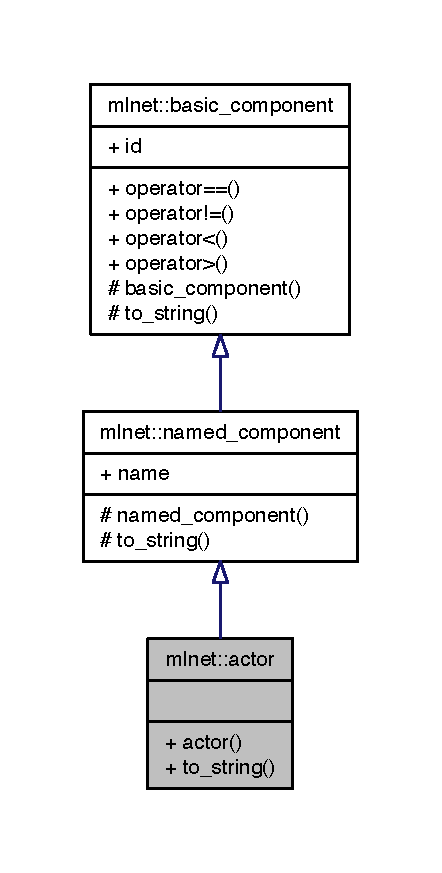
\includegraphics[width=212pt]{classmlnet_1_1actor__inherit__graph}
\end{center}
\end{figure}


Collaboration diagram for mlnet\+:\+:actor\+:\nopagebreak
\begin{figure}[H]
\begin{center}
\leavevmode
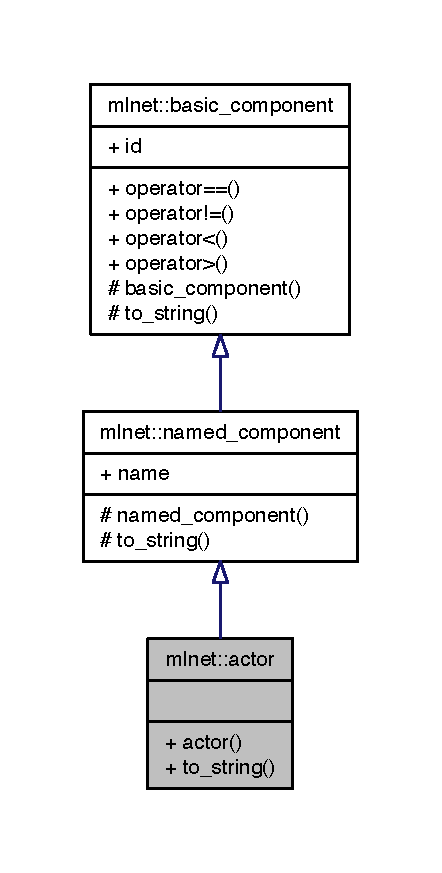
\includegraphics[width=212pt]{classmlnet_1_1actor__coll__graph}
\end{center}
\end{figure}
\subsection*{Public Member Functions}
\begin{DoxyCompactItemize}
\item 
\hyperlink{classmlnet_1_1actor_ab072eddf0e7e2182749c5cc3d59301b3}{actor} (const \hyperlink{namespacemlnet_a1d557bff46b627f1d7f6ff613302bba5}{actor\+\_\+id} \&\hyperlink{classmlnet_1_1basic__component_a7d56ea959ef686405bc0fa4830b03347}{id}, const std\+::string \&\hyperlink{classmlnet_1_1named__component_a3015f6650729352abae8fb01e7ee7ca7}{name})
\item 
std\+::string \hyperlink{classmlnet_1_1actor_a373ce265db390ecccc181d189520a075}{to\+\_\+string} () const 
\end{DoxyCompactItemize}
\subsection*{Additional Inherited Members}


\subsection{Detailed Description}
An actor in a \hyperlink{classmlnet_1_1_m_l_network}{M\+L\+Network}. 

\subsection{Constructor \& Destructor Documentation}
\hypertarget{classmlnet_1_1actor_ab072eddf0e7e2182749c5cc3d59301b3}{\index{mlnet\+::actor@{mlnet\+::actor}!actor@{actor}}
\index{actor@{actor}!mlnet\+::actor@{mlnet\+::actor}}
\subsubsection[{actor}]{\setlength{\rightskip}{0pt plus 5cm}mlnet\+::actor\+::actor (
\begin{DoxyParamCaption}
\item[{const {\bf actor\+\_\+id} \&}]{id, }
\item[{const std\+::string \&}]{name}
\end{DoxyParamCaption}
)}}\label{classmlnet_1_1actor_ab072eddf0e7e2182749c5cc3d59301b3}
Constructor 

\subsection{Member Function Documentation}
\hypertarget{classmlnet_1_1actor_a373ce265db390ecccc181d189520a075}{\index{mlnet\+::actor@{mlnet\+::actor}!to\+\_\+string@{to\+\_\+string}}
\index{to\+\_\+string@{to\+\_\+string}!mlnet\+::actor@{mlnet\+::actor}}
\subsubsection[{to\+\_\+string}]{\setlength{\rightskip}{0pt plus 5cm}std\+::string mlnet\+::actor\+::to\+\_\+string (
\begin{DoxyParamCaption}
{}
\end{DoxyParamCaption}
) const}}\label{classmlnet_1_1actor_a373ce265db390ecccc181d189520a075}
Output function, presenting a complete description of the actor 

The documentation for this class was generated from the following file\+:\begin{DoxyCompactItemize}
\item 
include/datastructures.\+h\end{DoxyCompactItemize}

\hypertarget{classmlnet_1_1_attribute}{\section{mlnet\+:\+:Attribute Class Reference}
\label{classmlnet_1_1_attribute}\index{mlnet\+::\+Attribute@{mlnet\+::\+Attribute}}
}


{\ttfamily \#include $<$datastructures.\+h$>$}



Collaboration diagram for mlnet\+:\+:Attribute\+:\nopagebreak
\begin{figure}[H]
\begin{center}
\leavevmode
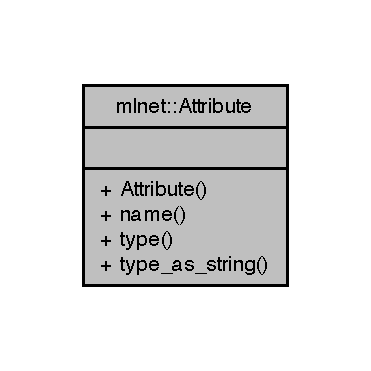
\includegraphics[width=178pt]{classmlnet_1_1_attribute__coll__graph}
\end{center}
\end{figure}
\subsection*{Public Member Functions}
\begin{DoxyCompactItemize}
\item 
\hyperlink{classmlnet_1_1_attribute_a51e4b9bb6f82914ffb6be78a4c28ab52}{Attribute} (const std\+::string \&\hyperlink{classmlnet_1_1_attribute_acac4019686c3a0a1c4362eea4d8e12e9}{name}, \hyperlink{namespacemlnet_a8bd10c6e8e4d27ef4d974b3f576a3a06}{attribute\+\_\+type} \hyperlink{classmlnet_1_1_attribute_ab9a7df6d77100640dfba5dcbf82aa977}{type})
\item 
const std\+::string \& \hyperlink{classmlnet_1_1_attribute_acac4019686c3a0a1c4362eea4d8e12e9}{name} () const 
\begin{DoxyCompactList}\small\item\em Returns the name of the attribute. \end{DoxyCompactList}\item 
int \hyperlink{classmlnet_1_1_attribute_ab9a7df6d77100640dfba5dcbf82aa977}{type} () const 
\begin{DoxyCompactList}\small\item\em Returns the type of the attribute. \end{DoxyCompactList}\item 
std\+::string \hyperlink{classmlnet_1_1_attribute_a0eb1239e4b715ce506129842387e5509}{type\+\_\+as\+\_\+string} () const 
\begin{DoxyCompactList}\small\item\em Returns a string representation of the type of the attribute. \end{DoxyCompactList}\end{DoxyCompactItemize}


\subsection{Detailed Description}
\hyperlink{classmlnet_1_1_attribute}{Attribute} handling Meta data about an attribute in an \hyperlink{classmlnet_1_1_attribute_store}{Attribute\+Store} 

\subsection{Constructor \& Destructor Documentation}
\hypertarget{classmlnet_1_1_attribute_a51e4b9bb6f82914ffb6be78a4c28ab52}{\index{mlnet\+::\+Attribute@{mlnet\+::\+Attribute}!Attribute@{Attribute}}
\index{Attribute@{Attribute}!mlnet\+::\+Attribute@{mlnet\+::\+Attribute}}
\subsubsection[{Attribute}]{\setlength{\rightskip}{0pt plus 5cm}mlnet\+::\+Attribute\+::\+Attribute (
\begin{DoxyParamCaption}
\item[{const std\+::string \&}]{name, }
\item[{{\bf attribute\+\_\+type}}]{type}
\end{DoxyParamCaption}
)}}\label{classmlnet_1_1_attribute_a51e4b9bb6f82914ffb6be78a4c28ab52}
Creates a new \hyperlink{classmlnet_1_1_attribute}{Attribute}. 
\begin{DoxyParams}{Parameters}
{\em name} & name of the attribute \\
\hline
{\em type} & type of the attribute (see attribute\+\_\+type enumeration\+: S\+T\+R\+I\+N\+G\+\_\+\+T\+Y\+P\+E, N\+U\+M\+E\+R\+I\+C\+\_\+\+T\+Y\+P\+E) \\
\hline
\end{DoxyParams}


\subsection{Member Function Documentation}
\hypertarget{classmlnet_1_1_attribute_acac4019686c3a0a1c4362eea4d8e12e9}{\index{mlnet\+::\+Attribute@{mlnet\+::\+Attribute}!name@{name}}
\index{name@{name}!mlnet\+::\+Attribute@{mlnet\+::\+Attribute}}
\subsubsection[{name}]{\setlength{\rightskip}{0pt plus 5cm}const std\+::string\& mlnet\+::\+Attribute\+::name (
\begin{DoxyParamCaption}
{}
\end{DoxyParamCaption}
) const}}\label{classmlnet_1_1_attribute_acac4019686c3a0a1c4362eea4d8e12e9}


Returns the name of the attribute. 

\begin{DoxyReturn}{Returns}
the name of the attribute. 
\end{DoxyReturn}
\hypertarget{classmlnet_1_1_attribute_ab9a7df6d77100640dfba5dcbf82aa977}{\index{mlnet\+::\+Attribute@{mlnet\+::\+Attribute}!type@{type}}
\index{type@{type}!mlnet\+::\+Attribute@{mlnet\+::\+Attribute}}
\subsubsection[{type}]{\setlength{\rightskip}{0pt plus 5cm}int mlnet\+::\+Attribute\+::type (
\begin{DoxyParamCaption}
{}
\end{DoxyParamCaption}
) const}}\label{classmlnet_1_1_attribute_ab9a7df6d77100640dfba5dcbf82aa977}


Returns the type of the attribute. 

\begin{DoxyReturn}{Returns}
the type of the attribute. 
\end{DoxyReturn}
\hypertarget{classmlnet_1_1_attribute_a0eb1239e4b715ce506129842387e5509}{\index{mlnet\+::\+Attribute@{mlnet\+::\+Attribute}!type\+\_\+as\+\_\+string@{type\+\_\+as\+\_\+string}}
\index{type\+\_\+as\+\_\+string@{type\+\_\+as\+\_\+string}!mlnet\+::\+Attribute@{mlnet\+::\+Attribute}}
\subsubsection[{type\+\_\+as\+\_\+string}]{\setlength{\rightskip}{0pt plus 5cm}std\+::string mlnet\+::\+Attribute\+::type\+\_\+as\+\_\+string (
\begin{DoxyParamCaption}
{}
\end{DoxyParamCaption}
) const}}\label{classmlnet_1_1_attribute_a0eb1239e4b715ce506129842387e5509}


Returns a string representation of the type of the attribute. 

\begin{DoxyReturn}{Returns}
a string representation of the type of the attribute. 
\end{DoxyReturn}


The documentation for this class was generated from the following file\+:\begin{DoxyCompactItemize}
\item 
include/datastructures.\+h\end{DoxyCompactItemize}

\hypertarget{classmlnet_1_1_attribute_store}{\section{mlnet\+:\+:Attribute\+Store Class Reference}
\label{classmlnet_1_1_attribute_store}\index{mlnet\+::\+Attribute\+Store@{mlnet\+::\+Attribute\+Store}}
}


{\ttfamily \#include $<$datastructures.\+h$>$}



Collaboration diagram for mlnet\+:\+:Attribute\+Store\+:\nopagebreak
\begin{figure}[H]
\begin{center}
\leavevmode
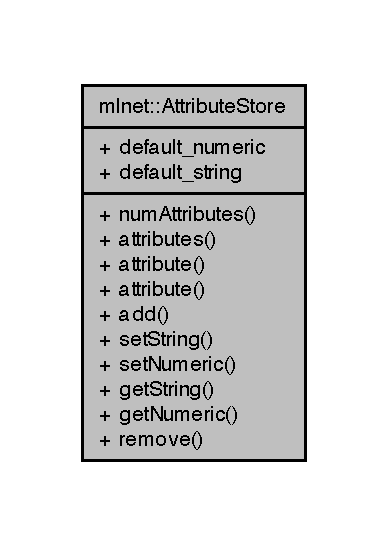
\includegraphics[width=186pt]{classmlnet_1_1_attribute_store__coll__graph}
\end{center}
\end{figure}
\subsection*{Public Member Functions}
\begin{DoxyCompactItemize}
\item 
int \hyperlink{classmlnet_1_1_attribute_store_a2c9be1aeffdebae76fc5abbd4f29ba49}{num\+Attributes} () const 
\begin{DoxyCompactList}\small\item\em Returns the number of attributes in this store, of all types. \end{DoxyCompactList}\item 
const std\+::vector\\*
$<$ \hyperlink{namespacemlnet_a760c8b8d6997e73350446bafff35e6d6}{Attribute\+Shared\+Ptr} $>$ \& \hyperlink{classmlnet_1_1_attribute_store_a6b1e02fe4782c546c69b8744e87cc715}{attributes} () const 
\begin{DoxyCompactList}\small\item\em Returns the attributes in this store. \end{DoxyCompactList}\item 
\hyperlink{namespacemlnet_a760c8b8d6997e73350446bafff35e6d6}{Attribute\+Shared\+Ptr} \hyperlink{classmlnet_1_1_attribute_store_abbb1d1393d05c7b9f50d24c99dab8313}{attribute} (int idx) const 
\begin{DoxyCompactList}\small\item\em Returns the n$^\wedge$th attribute in this store. \end{DoxyCompactList}\item 
\hyperlink{namespacemlnet_a760c8b8d6997e73350446bafff35e6d6}{Attribute\+Shared\+Ptr} \hyperlink{classmlnet_1_1_attribute_store_ab0a0e35a31e28573d3ec6292fa095acc}{attribute} (const std\+::string \&name) const 
\begin{DoxyCompactList}\small\item\em Returns an attribute by name. \end{DoxyCompactList}\item 
void \hyperlink{classmlnet_1_1_attribute_store_a9dbc93ccd1fd33d51cbad05aeee65ed0}{add} (const std\+::string \&attribute\+\_\+name, \hyperlink{namespacemlnet_a8bd10c6e8e4d27ef4d974b3f576a3a06}{attribute\+\_\+type} type)
\begin{DoxyCompactList}\small\item\em Enables the association of a value to each object in this store. \end{DoxyCompactList}\item 
void \hyperlink{classmlnet_1_1_attribute_store_a85f3fb59c476b2aeeeaee746fb9cb479}{set\+String} (const \hyperlink{namespacemlnet_a318fc9bfdb74e1da4d44d0c50d4a453d}{object\+\_\+id} \&id, const std\+::string \&attribute\+\_\+name, const std\+::string \&value)
\begin{DoxyCompactList}\small\item\em Sets the value of an attribute. \end{DoxyCompactList}\item 
void \hyperlink{classmlnet_1_1_attribute_store_a52c771c75c90c6d6a18a176d7c57d50e}{set\+Numeric} (const \hyperlink{namespacemlnet_a318fc9bfdb74e1da4d44d0c50d4a453d}{object\+\_\+id} \&id, const std\+::string \&attribute\+\_\+name, double value)
\begin{DoxyCompactList}\small\item\em Sets the value of an attribute. \end{DoxyCompactList}\item 
const std\+::string \& \hyperlink{classmlnet_1_1_attribute_store_acf03c80e6a33425ab4d61948bdd35c75}{get\+String} (const \hyperlink{namespacemlnet_a318fc9bfdb74e1da4d44d0c50d4a453d}{object\+\_\+id} \&id, const std\+::string \&attribute\+\_\+name) const 
\begin{DoxyCompactList}\small\item\em Gets the value of an attribute. \end{DoxyCompactList}\item 
const double \& \hyperlink{classmlnet_1_1_attribute_store_a42d014eb8df0be3bab9729bc906f650a}{get\+Numeric} (const \hyperlink{namespacemlnet_a318fc9bfdb74e1da4d44d0c50d4a453d}{object\+\_\+id} \&id, const std\+::string \&attribute\+\_\+name) const 
\begin{DoxyCompactList}\small\item\em Gets the value of an attribute. \end{DoxyCompactList}\item 
void \hyperlink{classmlnet_1_1_attribute_store_ad2f9528fdd74c4afcbcf50a03e320954}{remove} (const \hyperlink{namespacemlnet_a318fc9bfdb74e1da4d44d0c50d4a453d}{object\+\_\+id} \&id)
\begin{DoxyCompactList}\small\item\em Removes all the attribute values from an object. If the same object is queried after this method has been called, default values will be returned. \end{DoxyCompactList}\end{DoxyCompactItemize}
\subsection*{Public Attributes}
\begin{DoxyCompactItemize}
\item 
double \hyperlink{classmlnet_1_1_attribute_store_ac5843be6c280f09a18ded6030a85cfc5}{default\+\_\+numeric} = 0.\+0
\item 
std\+::string \hyperlink{classmlnet_1_1_attribute_store_a44894fedf9f2c0cb41d8af8ac270b0bb}{default\+\_\+string} = \char`\"{}\char`\"{}
\end{DoxyCompactItemize}


\subsection{Detailed Description}
A class associating multiple attributes and attribute values to a set of objects.

This class does not check if objects exist and does not require objects to be explicitly registered into it. Whenever an object that has not been explicitly registered is queried, default attribute values are returned. Therefore, checks about the existence of an object should be performed at the \hyperlink{classmlnet_1_1_m_l_network}{M\+L\+Network} level. 

\subsection{Member Function Documentation}
\hypertarget{classmlnet_1_1_attribute_store_a9dbc93ccd1fd33d51cbad05aeee65ed0}{\index{mlnet\+::\+Attribute\+Store@{mlnet\+::\+Attribute\+Store}!add@{add}}
\index{add@{add}!mlnet\+::\+Attribute\+Store@{mlnet\+::\+Attribute\+Store}}
\subsubsection[{add}]{\setlength{\rightskip}{0pt plus 5cm}void mlnet\+::\+Attribute\+Store\+::add (
\begin{DoxyParamCaption}
\item[{const std\+::string \&}]{attribute\+\_\+name, }
\item[{{\bf attribute\+\_\+type}}]{type}
\end{DoxyParamCaption}
)}}\label{classmlnet_1_1_attribute_store_a9dbc93ccd1fd33d51cbad05aeee65ed0}


Enables the association of a value to each object in this store. 


\begin{DoxyParams}{Parameters}
{\em attribute\+\_\+name} & The name of the attribute \\
\hline
{\em type} & The type of the attribute S\+T\+R\+I\+N\+G\+\_\+\+T\+Y\+P\+E\+: c++ \char`\"{}std\+::string\char`\"{} type N\+U\+M\+E\+R\+I\+C\+\_\+\+T\+Y\+P\+E\+: c++ \char`\"{}double\char`\"{} type \\
\hline
\end{DoxyParams}

\begin{DoxyExceptions}{Exceptions}
{\em \hyperlink{class_duplicate_element_exception}{Duplicate\+Element\+Exception}} & if an attribute with this name already exists \\
\hline
\end{DoxyExceptions}
\hypertarget{classmlnet_1_1_attribute_store_abbb1d1393d05c7b9f50d24c99dab8313}{\index{mlnet\+::\+Attribute\+Store@{mlnet\+::\+Attribute\+Store}!attribute@{attribute}}
\index{attribute@{attribute}!mlnet\+::\+Attribute\+Store@{mlnet\+::\+Attribute\+Store}}
\subsubsection[{attribute}]{\setlength{\rightskip}{0pt plus 5cm}{\bf Attribute\+Shared\+Ptr} mlnet\+::\+Attribute\+Store\+::attribute (
\begin{DoxyParamCaption}
\item[{int}]{idx}
\end{DoxyParamCaption}
) const}}\label{classmlnet_1_1_attribute_store_abbb1d1393d05c7b9f50d24c99dab8313}


Returns the n$^\wedge$th attribute in this store. 


\begin{DoxyParams}{Parameters}
{\em idx} & the position of the attribute (from 0 to \hyperlink{classmlnet_1_1_attribute_store_a2c9be1aeffdebae76fc5abbd4f29ba49}{num\+Attributes()}-\/1). \\
\hline
\end{DoxyParams}
\begin{DoxyReturn}{Returns}
an object of type \hyperlink{classmlnet_1_1_attribute}{Attribute}, or N\+U\+L\+L if idx's attribute does not exist. 
\end{DoxyReturn}
\hypertarget{classmlnet_1_1_attribute_store_ab0a0e35a31e28573d3ec6292fa095acc}{\index{mlnet\+::\+Attribute\+Store@{mlnet\+::\+Attribute\+Store}!attribute@{attribute}}
\index{attribute@{attribute}!mlnet\+::\+Attribute\+Store@{mlnet\+::\+Attribute\+Store}}
\subsubsection[{attribute}]{\setlength{\rightskip}{0pt plus 5cm}{\bf Attribute\+Shared\+Ptr} mlnet\+::\+Attribute\+Store\+::attribute (
\begin{DoxyParamCaption}
\item[{const std\+::string \&}]{name}
\end{DoxyParamCaption}
) const}}\label{classmlnet_1_1_attribute_store_ab0a0e35a31e28573d3ec6292fa095acc}


Returns an attribute by name. 


\begin{DoxyParams}{Parameters}
{\em name} & The name of the queried attribute. \\
\hline
\end{DoxyParams}
\begin{DoxyReturn}{Returns}
an object of type \hyperlink{classmlnet_1_1_attribute}{Attribute}, or N\+U\+L\+L if an attribute with this name does not exist. 
\end{DoxyReturn}
\hypertarget{classmlnet_1_1_attribute_store_a6b1e02fe4782c546c69b8744e87cc715}{\index{mlnet\+::\+Attribute\+Store@{mlnet\+::\+Attribute\+Store}!attributes@{attributes}}
\index{attributes@{attributes}!mlnet\+::\+Attribute\+Store@{mlnet\+::\+Attribute\+Store}}
\subsubsection[{attributes}]{\setlength{\rightskip}{0pt plus 5cm}const std\+::vector$<${\bf Attribute\+Shared\+Ptr}$>$\& mlnet\+::\+Attribute\+Store\+::attributes (
\begin{DoxyParamCaption}
{}
\end{DoxyParamCaption}
) const}}\label{classmlnet_1_1_attribute_store_a6b1e02fe4782c546c69b8744e87cc715}


Returns the attributes in this store. 

\begin{DoxyReturn}{Returns}
a vector containing all the attributes. 
\end{DoxyReturn}
\hypertarget{classmlnet_1_1_attribute_store_a42d014eb8df0be3bab9729bc906f650a}{\index{mlnet\+::\+Attribute\+Store@{mlnet\+::\+Attribute\+Store}!get\+Numeric@{get\+Numeric}}
\index{get\+Numeric@{get\+Numeric}!mlnet\+::\+Attribute\+Store@{mlnet\+::\+Attribute\+Store}}
\subsubsection[{get\+Numeric}]{\setlength{\rightskip}{0pt plus 5cm}const double\& mlnet\+::\+Attribute\+Store\+::get\+Numeric (
\begin{DoxyParamCaption}
\item[{const {\bf object\+\_\+id} \&}]{id, }
\item[{const std\+::string \&}]{attribute\+\_\+name}
\end{DoxyParamCaption}
) const}}\label{classmlnet_1_1_attribute_store_a42d014eb8df0be3bab9729bc906f650a}


Gets the value of an attribute. 


\begin{DoxyParams}{Parameters}
{\em id} & the id of the object whose associated value is retrieved \\
\hline
{\em attribute\+\_\+name} & The name of the attribute \\
\hline
\end{DoxyParams}

\begin{DoxyExceptions}{Exceptions}
{\em \hyperlink{class_element_not_found_exception}{Element\+Not\+Found\+Exception}} & if there is no object with this id \\
\hline
\end{DoxyExceptions}
\hypertarget{classmlnet_1_1_attribute_store_acf03c80e6a33425ab4d61948bdd35c75}{\index{mlnet\+::\+Attribute\+Store@{mlnet\+::\+Attribute\+Store}!get\+String@{get\+String}}
\index{get\+String@{get\+String}!mlnet\+::\+Attribute\+Store@{mlnet\+::\+Attribute\+Store}}
\subsubsection[{get\+String}]{\setlength{\rightskip}{0pt plus 5cm}const std\+::string\& mlnet\+::\+Attribute\+Store\+::get\+String (
\begin{DoxyParamCaption}
\item[{const {\bf object\+\_\+id} \&}]{id, }
\item[{const std\+::string \&}]{attribute\+\_\+name}
\end{DoxyParamCaption}
) const}}\label{classmlnet_1_1_attribute_store_acf03c80e6a33425ab4d61948bdd35c75}


Gets the value of an attribute. 


\begin{DoxyParams}{Parameters}
{\em id} & the id of the object whose associated value is retrieved \\
\hline
{\em attribute\+\_\+name} & The name of the attribute \\
\hline
\end{DoxyParams}
\begin{DoxyReturn}{Returns}
The value associated to the object, or null if the object id has not been registered in this store 
\end{DoxyReturn}

\begin{DoxyExceptions}{Exceptions}
{\em \hyperlink{class_element_not_found_exception}{Element\+Not\+Found\+Exception}} & if there is no attribute with this name \\
\hline
\end{DoxyExceptions}
\hypertarget{classmlnet_1_1_attribute_store_a2c9be1aeffdebae76fc5abbd4f29ba49}{\index{mlnet\+::\+Attribute\+Store@{mlnet\+::\+Attribute\+Store}!num\+Attributes@{num\+Attributes}}
\index{num\+Attributes@{num\+Attributes}!mlnet\+::\+Attribute\+Store@{mlnet\+::\+Attribute\+Store}}
\subsubsection[{num\+Attributes}]{\setlength{\rightskip}{0pt plus 5cm}int mlnet\+::\+Attribute\+Store\+::num\+Attributes (
\begin{DoxyParamCaption}
{}
\end{DoxyParamCaption}
) const}}\label{classmlnet_1_1_attribute_store_a2c9be1aeffdebae76fc5abbd4f29ba49}


Returns the number of attributes in this store, of all types. 

\begin{DoxyReturn}{Returns}
the number of attributes in this store 
\end{DoxyReturn}
\hypertarget{classmlnet_1_1_attribute_store_ad2f9528fdd74c4afcbcf50a03e320954}{\index{mlnet\+::\+Attribute\+Store@{mlnet\+::\+Attribute\+Store}!remove@{remove}}
\index{remove@{remove}!mlnet\+::\+Attribute\+Store@{mlnet\+::\+Attribute\+Store}}
\subsubsection[{remove}]{\setlength{\rightskip}{0pt plus 5cm}void mlnet\+::\+Attribute\+Store\+::remove (
\begin{DoxyParamCaption}
\item[{const {\bf object\+\_\+id} \&}]{id}
\end{DoxyParamCaption}
)}}\label{classmlnet_1_1_attribute_store_ad2f9528fdd74c4afcbcf50a03e320954}


Removes all the attribute values from an object. If the same object is queried after this method has been called, default values will be returned. 


\begin{DoxyParams}{Parameters}
{\em id} & The id of the object to be removed from the store. \\
\hline
\end{DoxyParams}
\hypertarget{classmlnet_1_1_attribute_store_a52c771c75c90c6d6a18a176d7c57d50e}{\index{mlnet\+::\+Attribute\+Store@{mlnet\+::\+Attribute\+Store}!set\+Numeric@{set\+Numeric}}
\index{set\+Numeric@{set\+Numeric}!mlnet\+::\+Attribute\+Store@{mlnet\+::\+Attribute\+Store}}
\subsubsection[{set\+Numeric}]{\setlength{\rightskip}{0pt plus 5cm}void mlnet\+::\+Attribute\+Store\+::set\+Numeric (
\begin{DoxyParamCaption}
\item[{const {\bf object\+\_\+id} \&}]{id, }
\item[{const std\+::string \&}]{attribute\+\_\+name, }
\item[{double}]{value}
\end{DoxyParamCaption}
)}}\label{classmlnet_1_1_attribute_store_a52c771c75c90c6d6a18a176d7c57d50e}


Sets the value of an attribute. 


\begin{DoxyParams}{Parameters}
{\em id} & the id of the object whose associated value is set \\
\hline
{\em attribute\+\_\+name} & The name of the attribute \\
\hline
{\em value} & The value to be set \\
\hline
\end{DoxyParams}

\begin{DoxyExceptions}{Exceptions}
{\em \hyperlink{class_element_not_found_exception}{Element\+Not\+Found\+Exception}} & if there is no attribute with this name \\
\hline
{\em \hyperlink{class_operation_not_supported_exception}{Operation\+Not\+Supported\+Exception}} & if the attribute type is not N\+U\+M\+E\+R\+I\+C\+\_\+\+T\+Y\+P\+E \\
\hline
\end{DoxyExceptions}
\hypertarget{classmlnet_1_1_attribute_store_a85f3fb59c476b2aeeeaee746fb9cb479}{\index{mlnet\+::\+Attribute\+Store@{mlnet\+::\+Attribute\+Store}!set\+String@{set\+String}}
\index{set\+String@{set\+String}!mlnet\+::\+Attribute\+Store@{mlnet\+::\+Attribute\+Store}}
\subsubsection[{set\+String}]{\setlength{\rightskip}{0pt plus 5cm}void mlnet\+::\+Attribute\+Store\+::set\+String (
\begin{DoxyParamCaption}
\item[{const {\bf object\+\_\+id} \&}]{id, }
\item[{const std\+::string \&}]{attribute\+\_\+name, }
\item[{const std\+::string \&}]{value}
\end{DoxyParamCaption}
)}}\label{classmlnet_1_1_attribute_store_a85f3fb59c476b2aeeeaee746fb9cb479}


Sets the value of an attribute. 


\begin{DoxyParams}{Parameters}
{\em id} & the id of the object whose associated value is set \\
\hline
{\em attribute\+\_\+name} & The name of the attribute \\
\hline
{\em value} & The value to be set \\
\hline
\end{DoxyParams}

\begin{DoxyExceptions}{Exceptions}
{\em \hyperlink{class_element_not_found_exception}{Element\+Not\+Found\+Exception}} & if there is no attribute with this name \\
\hline
{\em \hyperlink{class_operation_not_supported_exception}{Operation\+Not\+Supported\+Exception}} & if the attribute type is not S\+T\+R\+I\+N\+G\+\_\+\+T\+Y\+P\+E \\
\hline
\end{DoxyExceptions}


\subsection{Member Data Documentation}
\hypertarget{classmlnet_1_1_attribute_store_ac5843be6c280f09a18ded6030a85cfc5}{\index{mlnet\+::\+Attribute\+Store@{mlnet\+::\+Attribute\+Store}!default\+\_\+numeric@{default\+\_\+numeric}}
\index{default\+\_\+numeric@{default\+\_\+numeric}!mlnet\+::\+Attribute\+Store@{mlnet\+::\+Attribute\+Store}}
\subsubsection[{default\+\_\+numeric}]{\setlength{\rightskip}{0pt plus 5cm}double mlnet\+::\+Attribute\+Store\+::default\+\_\+numeric = 0.\+0}}\label{classmlnet_1_1_attribute_store_ac5843be6c280f09a18ded6030a85cfc5}
default value for numeric attributes \hypertarget{classmlnet_1_1_attribute_store_a44894fedf9f2c0cb41d8af8ac270b0bb}{\index{mlnet\+::\+Attribute\+Store@{mlnet\+::\+Attribute\+Store}!default\+\_\+string@{default\+\_\+string}}
\index{default\+\_\+string@{default\+\_\+string}!mlnet\+::\+Attribute\+Store@{mlnet\+::\+Attribute\+Store}}
\subsubsection[{default\+\_\+string}]{\setlength{\rightskip}{0pt plus 5cm}std\+::string mlnet\+::\+Attribute\+Store\+::default\+\_\+string = \char`\"{}\char`\"{}}}\label{classmlnet_1_1_attribute_store_a44894fedf9f2c0cb41d8af8ac270b0bb}
default value for string attributes 

The documentation for this class was generated from the following file\+:\begin{DoxyCompactItemize}
\item 
include/datastructures.\+h\end{DoxyCompactItemize}

\hypertarget{classmlnet_1_1_b_a_evolution_model}{\section{mlnet\+:\+:B\+A\+Evolution\+Model Class Reference}
\label{classmlnet_1_1_b_a_evolution_model}\index{mlnet\+::\+B\+A\+Evolution\+Model@{mlnet\+::\+B\+A\+Evolution\+Model}}
}


Grows a network by first creating a complete graph with m0 vertexes, then adding a new vertex at a time and connecting it to m other vertexes chosen with a probability proportional to their degree.  




{\ttfamily \#include $<$evolution.\+h$>$}



Inheritance diagram for mlnet\+:\+:B\+A\+Evolution\+Model\+:\nopagebreak
\begin{figure}[H]
\begin{center}
\leavevmode
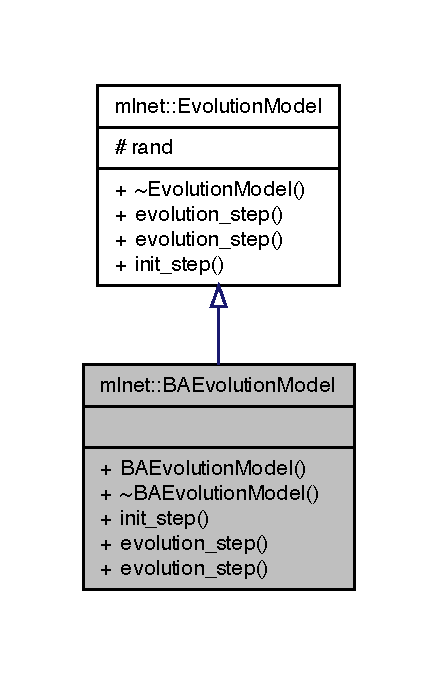
\includegraphics[width=210pt]{classmlnet_1_1_b_a_evolution_model__inherit__graph}
\end{center}
\end{figure}


Collaboration diagram for mlnet\+:\+:B\+A\+Evolution\+Model\+:\nopagebreak
\begin{figure}[H]
\begin{center}
\leavevmode
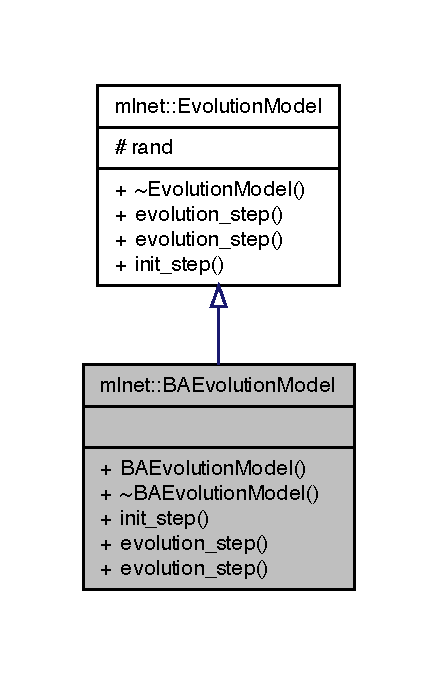
\includegraphics[width=210pt]{classmlnet_1_1_b_a_evolution_model__coll__graph}
\end{center}
\end{figure}
\subsection*{Public Member Functions}
\begin{DoxyCompactItemize}
\item 
\hypertarget{classmlnet_1_1_b_a_evolution_model_a8551399086c1ac90e583bc2859628776}{{\bfseries B\+A\+Evolution\+Model} (int m0, int m)}\label{classmlnet_1_1_b_a_evolution_model_a8551399086c1ac90e583bc2859628776}

\item 
\hypertarget{classmlnet_1_1_b_a_evolution_model_af4e5ec30340871601cb3228739ee44a4}{void {\bfseries init\+\_\+step} (\hyperlink{classmlnet_1_1_m_l_network}{M\+L\+Network} \&mnet, \hyperlink{namespacemlnet_a84ad9c6056f0eb7d129995351f9b13fb}{layer\+\_\+id} net)}\label{classmlnet_1_1_b_a_evolution_model_af4e5ec30340871601cb3228739ee44a4}

\item 
\hypertarget{classmlnet_1_1_b_a_evolution_model_a431911aa4a319849ea4d7f9ea2edc63e}{void {\bfseries evolution\+\_\+step} (\hyperlink{classmlnet_1_1_m_l_network}{M\+L\+Network} \&mnet, \hyperlink{namespacemlnet_a84ad9c6056f0eb7d129995351f9b13fb}{layer\+\_\+id} net)}\label{classmlnet_1_1_b_a_evolution_model_a431911aa4a319849ea4d7f9ea2edc63e}

\item 
\hypertarget{classmlnet_1_1_b_a_evolution_model_a59e23975027bfc11cedb3cb839e3916d}{void {\bfseries evolution\+\_\+step} (\hyperlink{classmlnet_1_1_m_l_network}{M\+L\+Network} \&mnet, \hyperlink{namespacemlnet_a84ad9c6056f0eb7d129995351f9b13fb}{layer\+\_\+id} net, std\+::set$<$ \hyperlink{namespacemlnet_a4c354f08ca868982bf3ddae882ff71c6}{node\+\_\+id} $>$ \&new\+\_\+vertexes, std\+::set$<$ \hyperlink{namespacemlnet_ad708e58e72680351e102e6b3d0489145}{edge\+\_\+id} $>$ \&new\+\_\+edges)}\label{classmlnet_1_1_b_a_evolution_model_a59e23975027bfc11cedb3cb839e3916d}

\end{DoxyCompactItemize}
\subsection*{Additional Inherited Members}


\subsection{Detailed Description}
Grows a network by first creating a complete graph with m0 vertexes, then adding a new vertex at a time and connecting it to m other vertexes chosen with a probability proportional to their degree. 

The documentation for this class was generated from the following file\+:\begin{DoxyCompactItemize}
\item 
include/evolution.\+h\end{DoxyCompactItemize}

\hypertarget{classmlnet_1_1basic__component}{\section{mlnet\+:\+:basic\+\_\+component Class Reference}
\label{classmlnet_1_1basic__component}\index{mlnet\+::basic\+\_\+component@{mlnet\+::basic\+\_\+component}}
}


{\ttfamily \#include $<$datastructures.\+h$>$}



Inheritance diagram for mlnet\+:\+:basic\+\_\+component\+:\nopagebreak
\begin{figure}[H]
\begin{center}
\leavevmode
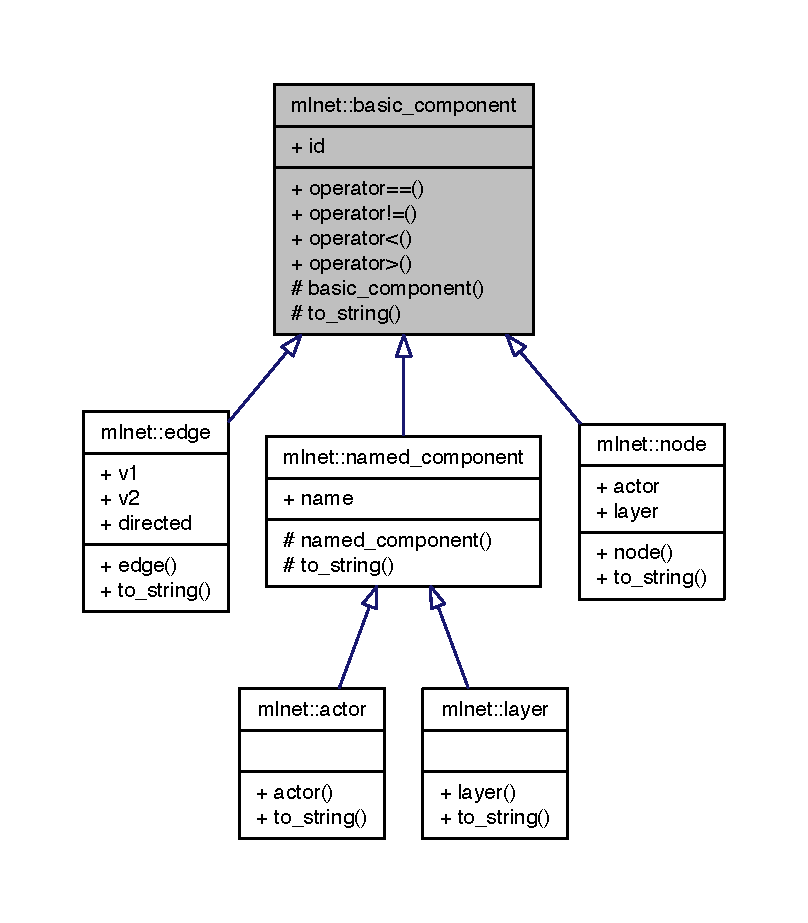
\includegraphics[width=350pt]{classmlnet_1_1basic__component__inherit__graph}
\end{center}
\end{figure}


Collaboration diagram for mlnet\+:\+:basic\+\_\+component\+:\nopagebreak
\begin{figure}[H]
\begin{center}
\leavevmode
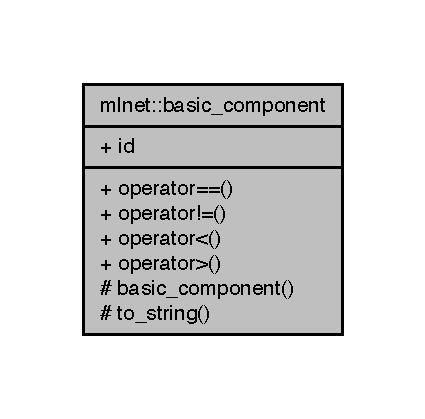
\includegraphics[width=204pt]{classmlnet_1_1basic__component__coll__graph}
\end{center}
\end{figure}
\subsection*{Public Member Functions}
\begin{DoxyCompactItemize}
\item 
bool \hyperlink{classmlnet_1_1basic__component_a468c756c9a5d625b49e2aa1f93b4c6a3}{operator==} (const \hyperlink{classmlnet_1_1basic__component}{basic\+\_\+component} \&comp) const 
\item 
bool \hyperlink{classmlnet_1_1basic__component_a17bdf6e789f07905a80e7d4f869092a5}{operator!=} (const \hyperlink{classmlnet_1_1basic__component}{basic\+\_\+component} \&comp) const 
\item 
bool \hyperlink{classmlnet_1_1basic__component_a6b85dec9c0f8275d0d25725dc03d64b9}{operator$<$} (const \hyperlink{classmlnet_1_1basic__component}{basic\+\_\+component} \&comp) const 
\item 
bool \hyperlink{classmlnet_1_1basic__component_acf2881d46bd20988ea48668d2e8ba2ff}{operator$>$} (const \hyperlink{classmlnet_1_1basic__component}{basic\+\_\+component} \&comp) const 
\end{DoxyCompactItemize}
\subsection*{Public Attributes}
\begin{DoxyCompactItemize}
\item 
const \hyperlink{namespacemlnet_a318fc9bfdb74e1da4d44d0c50d4a453d}{object\+\_\+id} \hyperlink{classmlnet_1_1basic__component_a7d56ea959ef686405bc0fa4830b03347}{id}
\end{DoxyCompactItemize}
\subsection*{Protected Member Functions}
\begin{DoxyCompactItemize}
\item 
\hyperlink{classmlnet_1_1basic__component_a72cb97290d5c73c64f43b4ce9e0891cf}{basic\+\_\+component} (const \hyperlink{namespacemlnet_a318fc9bfdb74e1da4d44d0c50d4a453d}{object\+\_\+id} \&\hyperlink{classmlnet_1_1basic__component_a7d56ea959ef686405bc0fa4830b03347}{id})
\item 
std\+::string \hyperlink{classmlnet_1_1basic__component_a533b88a0d280b70800f71b406b45d6f3}{to\+\_\+string} () const 
\end{DoxyCompactItemize}


\subsection{Detailed Description}
A generic basic component in a \hyperlink{classmlnet_1_1_m_l_network}{M\+L\+Network}. 

\subsection{Constructor \& Destructor Documentation}
\hypertarget{classmlnet_1_1basic__component_a72cb97290d5c73c64f43b4ce9e0891cf}{\index{mlnet\+::basic\+\_\+component@{mlnet\+::basic\+\_\+component}!basic\+\_\+component@{basic\+\_\+component}}
\index{basic\+\_\+component@{basic\+\_\+component}!mlnet\+::basic\+\_\+component@{mlnet\+::basic\+\_\+component}}
\subsubsection[{basic\+\_\+component}]{\setlength{\rightskip}{0pt plus 5cm}mlnet\+::basic\+\_\+component\+::basic\+\_\+component (
\begin{DoxyParamCaption}
\item[{const {\bf object\+\_\+id} \&}]{id}
\end{DoxyParamCaption}
)\hspace{0.3cm}{\ttfamily [protected]}}}\label{classmlnet_1_1basic__component_a72cb97290d5c73c64f43b4ce9e0891cf}
Constructor 

\subsection{Member Function Documentation}
\hypertarget{classmlnet_1_1basic__component_a17bdf6e789f07905a80e7d4f869092a5}{\index{mlnet\+::basic\+\_\+component@{mlnet\+::basic\+\_\+component}!operator"!=@{operator"!=}}
\index{operator"!=@{operator"!=}!mlnet\+::basic\+\_\+component@{mlnet\+::basic\+\_\+component}}
\subsubsection[{operator"!=}]{\setlength{\rightskip}{0pt plus 5cm}bool mlnet\+::basic\+\_\+component\+::operator!= (
\begin{DoxyParamCaption}
\item[{const {\bf basic\+\_\+component} \&}]{comp}
\end{DoxyParamCaption}
) const}}\label{classmlnet_1_1basic__component_a17bdf6e789f07905a80e7d4f869092a5}
Comparison operator\+: difference, based on the object identifiers. This assumes that objects of the same type are compared -\/ no checks are made for efficiency reasons. \hypertarget{classmlnet_1_1basic__component_a6b85dec9c0f8275d0d25725dc03d64b9}{\index{mlnet\+::basic\+\_\+component@{mlnet\+::basic\+\_\+component}!operator$<$@{operator$<$}}
\index{operator$<$@{operator$<$}!mlnet\+::basic\+\_\+component@{mlnet\+::basic\+\_\+component}}
\subsubsection[{operator$<$}]{\setlength{\rightskip}{0pt plus 5cm}bool mlnet\+::basic\+\_\+component\+::operator$<$ (
\begin{DoxyParamCaption}
\item[{const {\bf basic\+\_\+component} \&}]{comp}
\end{DoxyParamCaption}
) const}}\label{classmlnet_1_1basic__component_a6b85dec9c0f8275d0d25725dc03d64b9}
Comparison operator\+: less than, based on the object identifiers. This assumes that objects of the same type are compared -\/ no checks are made for efficiency reasons. \hypertarget{classmlnet_1_1basic__component_a468c756c9a5d625b49e2aa1f93b4c6a3}{\index{mlnet\+::basic\+\_\+component@{mlnet\+::basic\+\_\+component}!operator==@{operator==}}
\index{operator==@{operator==}!mlnet\+::basic\+\_\+component@{mlnet\+::basic\+\_\+component}}
\subsubsection[{operator==}]{\setlength{\rightskip}{0pt plus 5cm}bool mlnet\+::basic\+\_\+component\+::operator== (
\begin{DoxyParamCaption}
\item[{const {\bf basic\+\_\+component} \&}]{comp}
\end{DoxyParamCaption}
) const}}\label{classmlnet_1_1basic__component_a468c756c9a5d625b49e2aa1f93b4c6a3}
Comparison operator\+: equality, based on the object identifiers. This assumes that objects of the same type are compared -\/ no checks are made for efficiency reasons. \hypertarget{classmlnet_1_1basic__component_acf2881d46bd20988ea48668d2e8ba2ff}{\index{mlnet\+::basic\+\_\+component@{mlnet\+::basic\+\_\+component}!operator$>$@{operator$>$}}
\index{operator$>$@{operator$>$}!mlnet\+::basic\+\_\+component@{mlnet\+::basic\+\_\+component}}
\subsubsection[{operator$>$}]{\setlength{\rightskip}{0pt plus 5cm}bool mlnet\+::basic\+\_\+component\+::operator$>$ (
\begin{DoxyParamCaption}
\item[{const {\bf basic\+\_\+component} \&}]{comp}
\end{DoxyParamCaption}
) const}}\label{classmlnet_1_1basic__component_acf2881d46bd20988ea48668d2e8ba2ff}
Comparison operator\+: higher than, based on the object identifiers. This assumes that objects of the same type are compared -\/ no checks are made for efficiency reasons. \hypertarget{classmlnet_1_1basic__component_a533b88a0d280b70800f71b406b45d6f3}{\index{mlnet\+::basic\+\_\+component@{mlnet\+::basic\+\_\+component}!to\+\_\+string@{to\+\_\+string}}
\index{to\+\_\+string@{to\+\_\+string}!mlnet\+::basic\+\_\+component@{mlnet\+::basic\+\_\+component}}
\subsubsection[{to\+\_\+string}]{\setlength{\rightskip}{0pt plus 5cm}std\+::string mlnet\+::basic\+\_\+component\+::to\+\_\+string (
\begin{DoxyParamCaption}
{}
\end{DoxyParamCaption}
) const\hspace{0.3cm}{\ttfamily [protected]}}}\label{classmlnet_1_1basic__component_a533b88a0d280b70800f71b406b45d6f3}
Output function, presenting a complete description of the node 

\subsection{Member Data Documentation}
\hypertarget{classmlnet_1_1basic__component_a7d56ea959ef686405bc0fa4830b03347}{\index{mlnet\+::basic\+\_\+component@{mlnet\+::basic\+\_\+component}!id@{id}}
\index{id@{id}!mlnet\+::basic\+\_\+component@{mlnet\+::basic\+\_\+component}}
\subsubsection[{id}]{\setlength{\rightskip}{0pt plus 5cm}const {\bf object\+\_\+id} mlnet\+::basic\+\_\+component\+::id}}\label{classmlnet_1_1basic__component_a7d56ea959ef686405bc0fa4830b03347}
Unique identifier of the component 

The documentation for this class was generated from the following file\+:\begin{DoxyCompactItemize}
\item 
include/datastructures.\+h\end{DoxyCompactItemize}

\hypertarget{class_c_s_v_reader}{\section{C\+S\+V\+Reader Class Reference}
\label{class_c_s_v_reader}\index{C\+S\+V\+Reader@{C\+S\+V\+Reader}}
}


{\ttfamily \#include $<$utils.\+h$>$}



Collaboration diagram for C\+S\+V\+Reader\+:\nopagebreak
\begin{figure}[H]
\begin{center}
\leavevmode
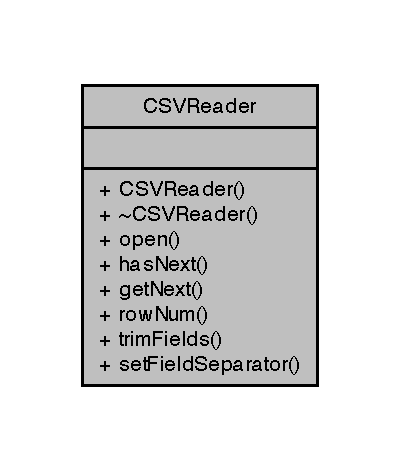
\includegraphics[width=192pt]{class_c_s_v_reader__coll__graph}
\end{center}
\end{figure}
\subsection*{Public Member Functions}
\begin{DoxyCompactItemize}
\item 
\hypertarget{class_c_s_v_reader_a26227ceca9cb3e5f761788e9934d4920}{void {\bfseries open} (std\+::string path)}\label{class_c_s_v_reader_a26227ceca9cb3e5f761788e9934d4920}

\item 
\hypertarget{class_c_s_v_reader_ae411eb74d89935e02287c499b28a36d6}{bool {\bfseries has\+Next} ()}\label{class_c_s_v_reader_ae411eb74d89935e02287c499b28a36d6}

\item 
\hypertarget{class_c_s_v_reader_a66d28a3bf8a3e4ef8a4c5f3fb2a238e8}{std\+::vector$<$ std\+::string $>$ {\bfseries get\+Next} ()}\label{class_c_s_v_reader_a66d28a3bf8a3e4ef8a4c5f3fb2a238e8}

\item 
\hypertarget{class_c_s_v_reader_a5a3d027966cb33b36c80070f6896c5ab}{int {\bfseries row\+Num} ()}\label{class_c_s_v_reader_a5a3d027966cb33b36c80070f6896c5ab}

\item 
\hypertarget{class_c_s_v_reader_aabd4741cea3e248340fe6a76f4ddd421}{void {\bfseries trim\+Fields} (bool value)}\label{class_c_s_v_reader_aabd4741cea3e248340fe6a76f4ddd421}

\item 
\hypertarget{class_c_s_v_reader_ae781c05f137c1745abbf03a7fe09d59a}{void {\bfseries set\+Field\+Separator} (char separator)}\label{class_c_s_v_reader_ae781c05f137c1745abbf03a7fe09d59a}

\end{DoxyCompactItemize}


\subsection{Detailed Description}
I\+O 

The documentation for this class was generated from the following file\+:\begin{DoxyCompactItemize}
\item 
include/utils.\+h\end{DoxyCompactItemize}

\hypertarget{classmlnet_1_1distance}{\section{mlnet\+:\+:distance Class Reference}
\label{classmlnet_1_1distance}\index{mlnet\+::distance@{mlnet\+::distance}}
}


{\ttfamily \#include $<$datastructures.\+h$>$}



Collaboration diagram for mlnet\+:\+:distance\+:
\nopagebreak
\begin{figure}[H]
\begin{center}
\leavevmode
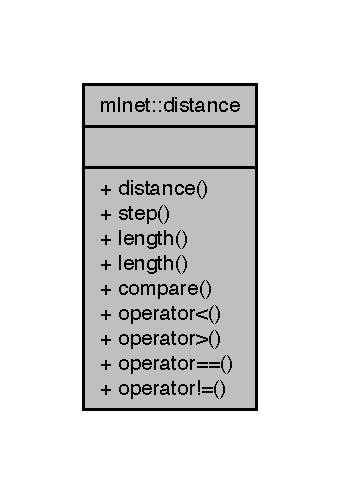
\includegraphics[width=163pt]{classmlnet_1_1distance__coll__graph}
\end{center}
\end{figure}
\subsection*{Public Member Functions}
\begin{DoxyCompactItemize}
\item 
\hyperlink{classmlnet_1_1distance_a51e12ba523084477376d511fd5e09cec}{distance} (const \hyperlink{namespacemlnet_aa6d3fa87865bcde4d1283abb1942cbbb}{M\+L\+Network\+Shared\+Ptr} \&mnet)
\item 
void \hyperlink{classmlnet_1_1distance_a84444db65304993aee043433d4230a5f}{step} (const \hyperlink{namespacemlnet_a33e88c3df9bea691a269d5e5d8bea57d}{Edge\+Shared\+Ptr} \&e)
\item 
long \hyperlink{classmlnet_1_1distance_ab4fbc7e9f6c432cc09c1746660e0ad77}{length} () const 
\item 
long \hyperlink{classmlnet_1_1distance_a9181679393e349f807c941d0b235c2a1}{length} (const \hyperlink{namespacemlnet_a84ad9c6056f0eb7d129995351f9b13fb}{layer\+\_\+id} \&from, const \hyperlink{namespacemlnet_a84ad9c6056f0eb7d129995351f9b13fb}{layer\+\_\+id} \&to) const 
\item 
\hyperlink{namespacemlnet_a49cbf481a06184d43958acdfc5d4fc60}{domination} \hyperlink{classmlnet_1_1distance_a713d9d390380246f1baf1cae2c1985f6}{compare} (const \hyperlink{classmlnet_1_1distance}{distance} \&other, \hyperlink{namespacemlnet_ac59b03c9fd702da21a0c3c2a4bba57c9}{comparison\+\_\+type} comp) const 
\begin{DoxyCompactList}\small\item\em Compares two distances according to the comp parameter\+: \end{DoxyCompactList}\item 
bool \hyperlink{classmlnet_1_1distance_ab9376eda4dcc818d9d656c002945c574}{operator$<$} (const \hyperlink{classmlnet_1_1distance}{distance} \&other) const 
\item 
bool \hyperlink{classmlnet_1_1distance_ac401f9433fa0533b5aa068bce4967c92}{operator$>$} (const \hyperlink{classmlnet_1_1distance}{distance} \&other) const 
\item 
bool \hyperlink{classmlnet_1_1distance_ac410d457518bf8f13873b6e3324ef18b}{operator==} (const \hyperlink{classmlnet_1_1distance}{distance} \&other) const 
\item 
bool \hyperlink{classmlnet_1_1distance_ad5e31fdb75840e134b9dc7662ad11e4c}{operator!=} (const \hyperlink{classmlnet_1_1distance}{distance} \&other) const 
\end{DoxyCompactItemize}


\subsection{Detailed Description}
This class represents a sequence of consecutive edges in a multilayer network. 

\subsection{Constructor \& Destructor Documentation}
\hypertarget{classmlnet_1_1distance_a51e12ba523084477376d511fd5e09cec}{\index{mlnet\+::distance@{mlnet\+::distance}!distance@{distance}}
\index{distance@{distance}!mlnet\+::distance@{mlnet\+::distance}}
\subsubsection[{distance}]{\setlength{\rightskip}{0pt plus 5cm}mlnet\+::distance\+::distance (
\begin{DoxyParamCaption}
\item[{const {\bf M\+L\+Network\+Shared\+Ptr} \&}]{mnet}
\end{DoxyParamCaption}
)}}\label{classmlnet_1_1distance_a51e12ba523084477376d511fd5e09cec}
Constructs an empty distance. 

\subsection{Member Function Documentation}
\hypertarget{classmlnet_1_1distance_a713d9d390380246f1baf1cae2c1985f6}{\index{mlnet\+::distance@{mlnet\+::distance}!compare@{compare}}
\index{compare@{compare}!mlnet\+::distance@{mlnet\+::distance}}
\subsubsection[{compare}]{\setlength{\rightskip}{0pt plus 5cm}{\bf domination} mlnet\+::distance\+::compare (
\begin{DoxyParamCaption}
\item[{const {\bf distance} \&}]{other, }
\item[{{\bf comparison\+\_\+type}}]{comp}
\end{DoxyParamCaption}
) const}}\label{classmlnet_1_1distance_a713d9d390380246f1baf1cae2c1985f6}


Compares two distances according to the comp parameter\+: 


\begin{DoxyParams}{Parameters}
{\em other} & The distance to be compared to. \\
\hline
{\em comp} & This parameter specifies the amount of information used while comparing the two distances\+:
\begin{DoxyItemize}
\item F\+U\+L\+L\+\_\+\+C\+O\+M\+P\+A\+R\+I\+S\+O\+N\+: all steps among each pair of layers (including the same layer) are considered as distinct entities, and a Pareto relationship is returned (that is, the two distances may be incomparable).
\item S\+W\+I\+T\+C\+H\+\_\+\+C\+O\+M\+P\+A\+R\+I\+S\+O\+N\+: all steps inside the same layer and the steps between any two different layers are considered as distinct entities, and a Pareto relationship is returned (that is, the two distances may be incomparable).
\item M\+U\+L\+T\+I\+P\+L\+E\+X\+\_\+\+C\+O\+M\+P\+A\+R\+I\+S\+O\+N\+: all steps inside the same layer are considered as distinct entities. Inter-\/layer steps are not counted, and a Pareto relationship is returned (that is, the two distances may be incomparable).
\item S\+I\+M\+P\+L\+E\+\_\+\+C\+O\+M\+P\+A\+R\+I\+S\+O\+N\+: the total number of steps is considered. The two distances will always be comparable ($<$, $>$, == or !=). 
\end{DoxyItemize}\\
\hline
\end{DoxyParams}
\begin{DoxyReturn}{Returns}
One of the relationship types\+: P\+\_\+\+D\+O\+M\+I\+N\+A\+T\+E\+D, P\+\_\+\+E\+Q\+U\+A\+L, P\+\_\+\+I\+N\+C\+O\+M\+P\+A\+R\+A\+B\+L\+E, or P\+\_\+\+D\+O\+M\+I\+N\+A\+T\+E\+S 
\end{DoxyReturn}
\hypertarget{classmlnet_1_1distance_ab4fbc7e9f6c432cc09c1746660e0ad77}{\index{mlnet\+::distance@{mlnet\+::distance}!length@{length}}
\index{length@{length}!mlnet\+::distance@{mlnet\+::distance}}
\subsubsection[{length}]{\setlength{\rightskip}{0pt plus 5cm}long mlnet\+::distance\+::length (
\begin{DoxyParamCaption}
{}
\end{DoxyParamCaption}
) const}}\label{classmlnet_1_1distance_ab4fbc7e9f6c432cc09c1746660e0ad77}
\begin{DoxyReturn}{Returns}
The total number of steps (that is, traversed edges). 
\end{DoxyReturn}
\hypertarget{classmlnet_1_1distance_a9181679393e349f807c941d0b235c2a1}{\index{mlnet\+::distance@{mlnet\+::distance}!length@{length}}
\index{length@{length}!mlnet\+::distance@{mlnet\+::distance}}
\subsubsection[{length}]{\setlength{\rightskip}{0pt plus 5cm}long mlnet\+::distance\+::length (
\begin{DoxyParamCaption}
\item[{const {\bf layer\+\_\+id} \&}]{from, }
\item[{const {\bf layer\+\_\+id} \&}]{to}
\end{DoxyParamCaption}
) const}}\label{classmlnet_1_1distance_a9181679393e349f807c941d0b235c2a1}
\begin{DoxyReturn}{Returns}
The number of steps (that is, traversed edges) from a node in layer from to a node in layer to. 
\end{DoxyReturn}

\begin{DoxyParams}{Parameters}
{\em from} & first layer. \\
\hline
{\em to} & second layer. \\
\hline
\end{DoxyParams}
\hypertarget{classmlnet_1_1distance_ad5e31fdb75840e134b9dc7662ad11e4c}{\index{mlnet\+::distance@{mlnet\+::distance}!operator"!=@{operator"!=}}
\index{operator"!=@{operator"!=}!mlnet\+::distance@{mlnet\+::distance}}
\subsubsection[{operator"!=}]{\setlength{\rightskip}{0pt plus 5cm}bool mlnet\+::distance\+::operator!= (
\begin{DoxyParamCaption}
\item[{const {\bf distance} \&}]{other}
\end{DoxyParamCaption}
) const}}\label{classmlnet_1_1distance_ad5e31fdb75840e134b9dc7662ad11e4c}
Compare the absolute length of the two distances. For a comparison considering steps on different layers as incomparable entities, use \hyperlink{classmlnet_1_1distance_a713d9d390380246f1baf1cae2c1985f6}{compare()} 
\begin{DoxyParams}{Parameters}
{\em other} & The distance to be compared to. \\
\hline
\end{DoxyParams}
\begin{DoxyReturn}{Returns}
true if this distance is different from the input one. 
\end{DoxyReturn}
\hypertarget{classmlnet_1_1distance_ab9376eda4dcc818d9d656c002945c574}{\index{mlnet\+::distance@{mlnet\+::distance}!operator$<$@{operator$<$}}
\index{operator$<$@{operator$<$}!mlnet\+::distance@{mlnet\+::distance}}
\subsubsection[{operator$<$}]{\setlength{\rightskip}{0pt plus 5cm}bool mlnet\+::distance\+::operator$<$ (
\begin{DoxyParamCaption}
\item[{const {\bf distance} \&}]{other}
\end{DoxyParamCaption}
) const}}\label{classmlnet_1_1distance_ab9376eda4dcc818d9d656c002945c574}
Compare the absolute length of the two distances. For a comparison considering steps on different layers as incomparable entities, use \hyperlink{classmlnet_1_1distance_a713d9d390380246f1baf1cae2c1985f6}{compare()} 
\begin{DoxyParams}{Parameters}
{\em other} & The distance to be compared to. \\
\hline
\end{DoxyParams}
\begin{DoxyReturn}{Returns}
true if this distance is shorter than the input one. 
\end{DoxyReturn}
\hypertarget{classmlnet_1_1distance_ac410d457518bf8f13873b6e3324ef18b}{\index{mlnet\+::distance@{mlnet\+::distance}!operator==@{operator==}}
\index{operator==@{operator==}!mlnet\+::distance@{mlnet\+::distance}}
\subsubsection[{operator==}]{\setlength{\rightskip}{0pt plus 5cm}bool mlnet\+::distance\+::operator== (
\begin{DoxyParamCaption}
\item[{const {\bf distance} \&}]{other}
\end{DoxyParamCaption}
) const}}\label{classmlnet_1_1distance_ac410d457518bf8f13873b6e3324ef18b}
Compare the absolute length of the two distances. For a comparison considering steps on different layers as incomparable entities, use \hyperlink{classmlnet_1_1distance_a713d9d390380246f1baf1cae2c1985f6}{compare()} 
\begin{DoxyParams}{Parameters}
{\em other} & The distance to be compared to. \\
\hline
\end{DoxyParams}
\begin{DoxyReturn}{Returns}
true if this distance is the same as the input one. 
\end{DoxyReturn}
\hypertarget{classmlnet_1_1distance_ac401f9433fa0533b5aa068bce4967c92}{\index{mlnet\+::distance@{mlnet\+::distance}!operator$>$@{operator$>$}}
\index{operator$>$@{operator$>$}!mlnet\+::distance@{mlnet\+::distance}}
\subsubsection[{operator$>$}]{\setlength{\rightskip}{0pt plus 5cm}bool mlnet\+::distance\+::operator$>$ (
\begin{DoxyParamCaption}
\item[{const {\bf distance} \&}]{other}
\end{DoxyParamCaption}
) const}}\label{classmlnet_1_1distance_ac401f9433fa0533b5aa068bce4967c92}
Compare the absolute length of the two distances. For a comparison considering steps on different layers as incomparable entities, use \hyperlink{classmlnet_1_1distance_a713d9d390380246f1baf1cae2c1985f6}{compare()} 
\begin{DoxyParams}{Parameters}
{\em other} & The distance to be compared to. \\
\hline
\end{DoxyParams}
\begin{DoxyReturn}{Returns}
true if this distance is longer than the input one. 
\end{DoxyReturn}
\hypertarget{classmlnet_1_1distance_a84444db65304993aee043433d4230a5f}{\index{mlnet\+::distance@{mlnet\+::distance}!step@{step}}
\index{step@{step}!mlnet\+::distance@{mlnet\+::distance}}
\subsubsection[{step}]{\setlength{\rightskip}{0pt plus 5cm}void mlnet\+::distance\+::step (
\begin{DoxyParamCaption}
\item[{const {\bf Edge\+Shared\+Ptr} \&}]{e}
\end{DoxyParamCaption}
)}}\label{classmlnet_1_1distance_a84444db65304993aee043433d4230a5f}
Increases this distance. 
\begin{DoxyParams}{Parameters}
{\em e} & an edge indicating a new step to be added to the distance. \\
\hline
\end{DoxyParams}


The documentation for this class was generated from the following file\+:\begin{DoxyCompactItemize}
\item 
include/datastructures.\+h\end{DoxyCompactItemize}

\hypertarget{class_duplicate_element_exception}{\section{Duplicate\+Element\+Exception Class Reference}
\label{class_duplicate_element_exception}\index{Duplicate\+Element\+Exception@{Duplicate\+Element\+Exception}}
}


Inheritance diagram for Duplicate\+Element\+Exception\+:\nopagebreak
\begin{figure}[H]
\begin{center}
\leavevmode
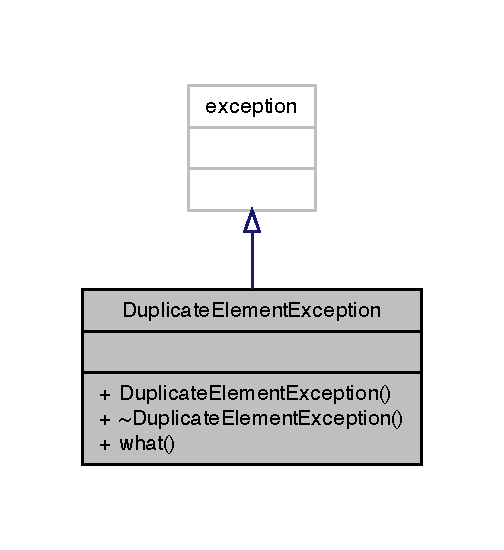
\includegraphics[width=242pt]{class_duplicate_element_exception__inherit__graph}
\end{center}
\end{figure}


Collaboration diagram for Duplicate\+Element\+Exception\+:\nopagebreak
\begin{figure}[H]
\begin{center}
\leavevmode
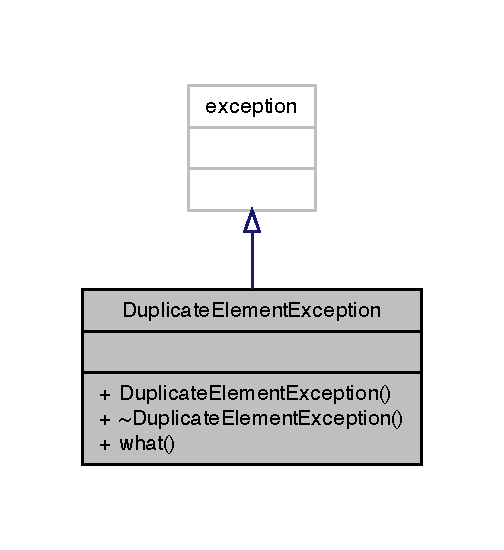
\includegraphics[width=242pt]{class_duplicate_element_exception__coll__graph}
\end{center}
\end{figure}
\subsection*{Public Member Functions}
\begin{DoxyCompactItemize}
\item 
\hypertarget{class_duplicate_element_exception_ab1804ab13d350d893d3d003f13035232}{{\bfseries Duplicate\+Element\+Exception} (std\+::string value)}\label{class_duplicate_element_exception_ab1804ab13d350d893d3d003f13035232}

\item 
\hypertarget{class_duplicate_element_exception_a5021dd1ab2a52d557f04e55fb792de47}{virtual const char $\ast$ {\bfseries what} () const   throw ()}\label{class_duplicate_element_exception_a5021dd1ab2a52d557f04e55fb792de47}

\end{DoxyCompactItemize}


The documentation for this class was generated from the following file\+:\begin{DoxyCompactItemize}
\item 
include/exceptions.\+h\end{DoxyCompactItemize}

\hypertarget{classmlnet_1_1edge}{\section{mlnet\+:\+:edge Class Reference}
\label{classmlnet_1_1edge}\index{mlnet\+::edge@{mlnet\+::edge}}
}


{\ttfamily \#include $<$datastructures.\+h$>$}



Inheritance diagram for mlnet\+:\+:edge\+:\nopagebreak
\begin{figure}[H]
\begin{center}
\leavevmode
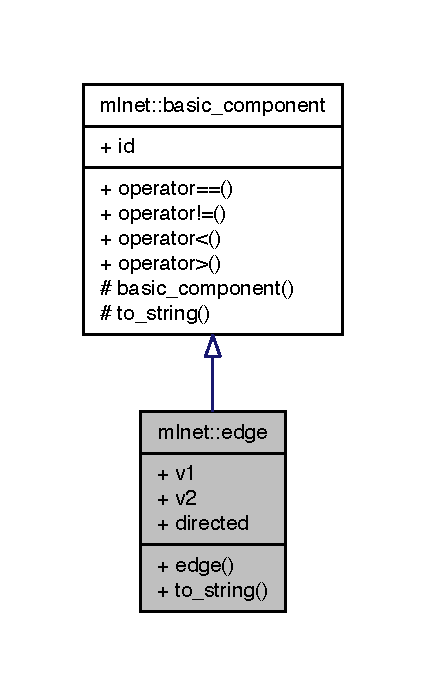
\includegraphics[width=204pt]{classmlnet_1_1edge__inherit__graph}
\end{center}
\end{figure}


Collaboration diagram for mlnet\+:\+:edge\+:\nopagebreak
\begin{figure}[H]
\begin{center}
\leavevmode
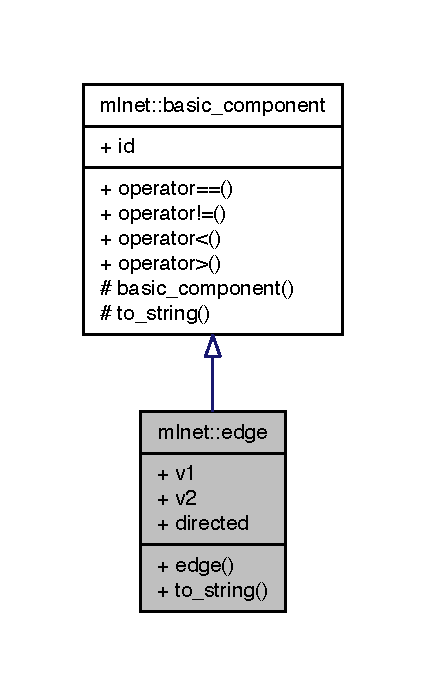
\includegraphics[width=204pt]{classmlnet_1_1edge__coll__graph}
\end{center}
\end{figure}
\subsection*{Public Member Functions}
\begin{DoxyCompactItemize}
\item 
\hyperlink{classmlnet_1_1edge_a1b81e36ac55205d1aca6cbde4679a794}{edge} (const \hyperlink{namespacemlnet_ad708e58e72680351e102e6b3d0489145}{edge\+\_\+id} \&\hyperlink{classmlnet_1_1basic__component_a7d56ea959ef686405bc0fa4830b03347}{id}, const \hyperlink{namespacemlnet_acf8b1b6deb52e7dacfc676c689f9a10c}{Node\+Shared\+Ptr} \&\hyperlink{classmlnet_1_1edge_a5937b3d8aaa623600d68c3389e1bcfbc}{v1}, const \hyperlink{namespacemlnet_acf8b1b6deb52e7dacfc676c689f9a10c}{Node\+Shared\+Ptr} \&\hyperlink{classmlnet_1_1edge_ac9c3f96b25b4f06cf3d2202e8ea661dc}{v2}, bool \hyperlink{classmlnet_1_1edge_a317e58d611d421b7a2472a9b0e47da3b}{directed})
\item 
std\+::string \hyperlink{classmlnet_1_1edge_a070bcf02c3d765f910fbd0eef40d6ff1}{to\+\_\+string} () const 
\end{DoxyCompactItemize}
\subsection*{Public Attributes}
\begin{DoxyCompactItemize}
\item 
\hyperlink{namespacemlnet_acf8b1b6deb52e7dacfc676c689f9a10c}{Node\+Shared\+Ptr} \hyperlink{classmlnet_1_1edge_a5937b3d8aaa623600d68c3389e1bcfbc}{v1}
\item 
\hyperlink{namespacemlnet_acf8b1b6deb52e7dacfc676c689f9a10c}{Node\+Shared\+Ptr} \hyperlink{classmlnet_1_1edge_ac9c3f96b25b4f06cf3d2202e8ea661dc}{v2}
\item 
bool \hyperlink{classmlnet_1_1edge_a317e58d611d421b7a2472a9b0e47da3b}{directed}
\end{DoxyCompactItemize}
\subsection*{Additional Inherited Members}


\subsection{Detailed Description}
An edge between two nodes in a \hyperlink{classmlnet_1_1_m_l_network}{M\+L\+Network}. 

\subsection{Constructor \& Destructor Documentation}
\hypertarget{classmlnet_1_1edge_a1b81e36ac55205d1aca6cbde4679a794}{\index{mlnet\+::edge@{mlnet\+::edge}!edge@{edge}}
\index{edge@{edge}!mlnet\+::edge@{mlnet\+::edge}}
\subsubsection[{edge}]{\setlength{\rightskip}{0pt plus 5cm}mlnet\+::edge\+::edge (
\begin{DoxyParamCaption}
\item[{const {\bf edge\+\_\+id} \&}]{id, }
\item[{const {\bf Node\+Shared\+Ptr} \&}]{v1, }
\item[{const {\bf Node\+Shared\+Ptr} \&}]{v2, }
\item[{bool}]{directed}
\end{DoxyParamCaption}
)}}\label{classmlnet_1_1edge_a1b81e36ac55205d1aca6cbde4679a794}
Constructor 

\subsection{Member Function Documentation}
\hypertarget{classmlnet_1_1edge_a070bcf02c3d765f910fbd0eef40d6ff1}{\index{mlnet\+::edge@{mlnet\+::edge}!to\+\_\+string@{to\+\_\+string}}
\index{to\+\_\+string@{to\+\_\+string}!mlnet\+::edge@{mlnet\+::edge}}
\subsubsection[{to\+\_\+string}]{\setlength{\rightskip}{0pt plus 5cm}std\+::string mlnet\+::edge\+::to\+\_\+string (
\begin{DoxyParamCaption}
{}
\end{DoxyParamCaption}
) const}}\label{classmlnet_1_1edge_a070bcf02c3d765f910fbd0eef40d6ff1}
Output function, presenting a complete description of the edge 

\subsection{Member Data Documentation}
\hypertarget{classmlnet_1_1edge_a317e58d611d421b7a2472a9b0e47da3b}{\index{mlnet\+::edge@{mlnet\+::edge}!directed@{directed}}
\index{directed@{directed}!mlnet\+::edge@{mlnet\+::edge}}
\subsubsection[{directed}]{\setlength{\rightskip}{0pt plus 5cm}bool mlnet\+::edge\+::directed}}\label{classmlnet_1_1edge_a317e58d611d421b7a2472a9b0e47da3b}
Edge directionality \hypertarget{classmlnet_1_1edge_a5937b3d8aaa623600d68c3389e1bcfbc}{\index{mlnet\+::edge@{mlnet\+::edge}!v1@{v1}}
\index{v1@{v1}!mlnet\+::edge@{mlnet\+::edge}}
\subsubsection[{v1}]{\setlength{\rightskip}{0pt plus 5cm}{\bf Node\+Shared\+Ptr} mlnet\+::edge\+::v1}}\label{classmlnet_1_1edge_a5937b3d8aaa623600d68c3389e1bcfbc}
The node at the first end of this edge \hypertarget{classmlnet_1_1edge_ac9c3f96b25b4f06cf3d2202e8ea661dc}{\index{mlnet\+::edge@{mlnet\+::edge}!v2@{v2}}
\index{v2@{v2}!mlnet\+::edge@{mlnet\+::edge}}
\subsubsection[{v2}]{\setlength{\rightskip}{0pt plus 5cm}{\bf Node\+Shared\+Ptr} mlnet\+::edge\+::v2}}\label{classmlnet_1_1edge_ac9c3f96b25b4f06cf3d2202e8ea661dc}
The node at the second end of this edge 

The documentation for this class was generated from the following file\+:\begin{DoxyCompactItemize}
\item 
include/datastructures.\+h\end{DoxyCompactItemize}

\hypertarget{class_element_not_found_exception}{\section{Element\+Not\+Found\+Exception Class Reference}
\label{class_element_not_found_exception}\index{Element\+Not\+Found\+Exception@{Element\+Not\+Found\+Exception}}
}


Inheritance diagram for Element\+Not\+Found\+Exception\+:\nopagebreak
\begin{figure}[H]
\begin{center}
\leavevmode
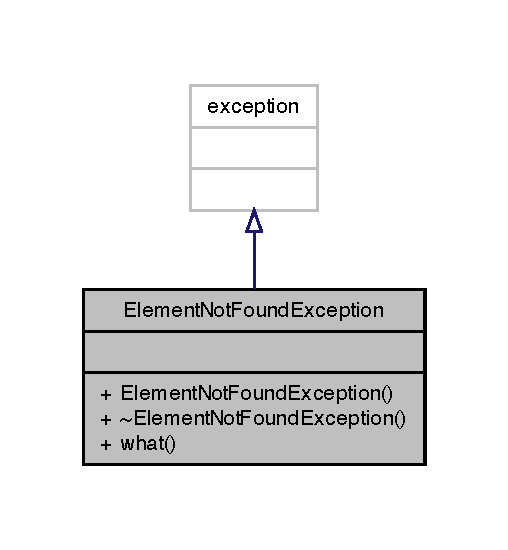
\includegraphics[width=244pt]{class_element_not_found_exception__inherit__graph}
\end{center}
\end{figure}


Collaboration diagram for Element\+Not\+Found\+Exception\+:\nopagebreak
\begin{figure}[H]
\begin{center}
\leavevmode
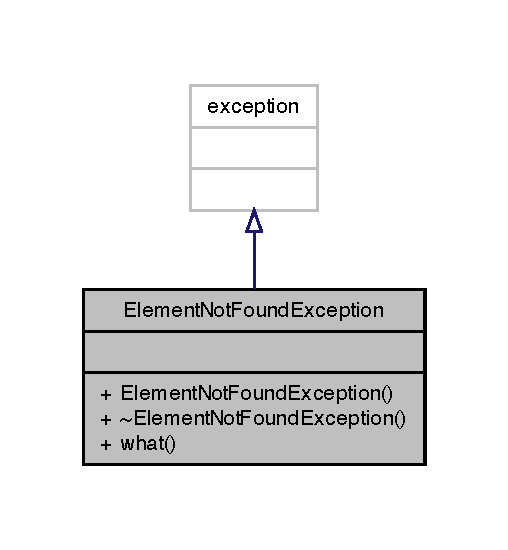
\includegraphics[width=244pt]{class_element_not_found_exception__coll__graph}
\end{center}
\end{figure}
\subsection*{Public Member Functions}
\begin{DoxyCompactItemize}
\item 
\hypertarget{class_element_not_found_exception_ad21e23268542ce1670189a97ac9a355d}{{\bfseries Element\+Not\+Found\+Exception} (std\+::string value)}\label{class_element_not_found_exception_ad21e23268542ce1670189a97ac9a355d}

\item 
\hypertarget{class_element_not_found_exception_a96cadc7c34010e185b32d230974b4f40}{virtual const char $\ast$ {\bfseries what} () const   throw ()}\label{class_element_not_found_exception_a96cadc7c34010e185b32d230974b4f40}

\end{DoxyCompactItemize}


The documentation for this class was generated from the following file\+:\begin{DoxyCompactItemize}
\item 
include/exceptions.\+h\end{DoxyCompactItemize}

\hypertarget{classmlnet_1_1_entry}{\section{mlnet\+:\+:Entry$<$ T $>$ Class Template Reference}
\label{classmlnet_1_1_entry}\index{mlnet\+::\+Entry$<$ T $>$@{mlnet\+::\+Entry$<$ T $>$}}
}


{\ttfamily \#include $<$datastructures.\+h$>$}



Inheritance diagram for mlnet\+:\+:Entry$<$ T $>$\+:\nopagebreak
\begin{figure}[H]
\begin{center}
\leavevmode
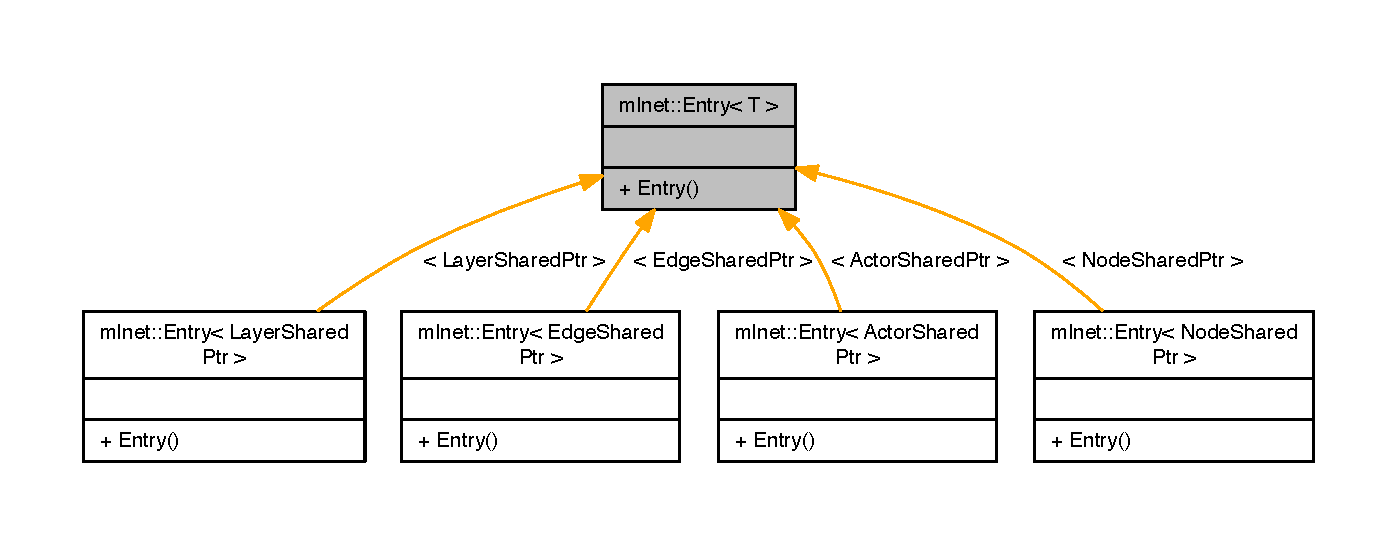
\includegraphics[width=350pt]{classmlnet_1_1_entry__inherit__graph}
\end{center}
\end{figure}


Collaboration diagram for mlnet\+:\+:Entry$<$ T $>$\+:\nopagebreak
\begin{figure}[H]
\begin{center}
\leavevmode
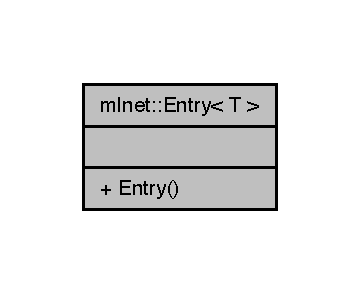
\includegraphics[width=173pt]{classmlnet_1_1_entry__coll__graph}
\end{center}
\end{figure}
\subsection*{Public Member Functions}
\begin{DoxyCompactItemize}
\item 
\hyperlink{classmlnet_1_1_entry_a61aa2a28da149dd5ff9e5137560ba71f}{Entry} (int level, \hyperlink{namespacemlnet_a318fc9bfdb74e1da4d44d0c50d4a453d}{object\+\_\+id} id, T obj)
\end{DoxyCompactItemize}
\subsection*{Friends}
\begin{DoxyCompactItemize}
\item 
\hypertarget{classmlnet_1_1_entry_aedfb12ef9f1601d05985fca601062388}{class {\bfseries Sorted\+Set$<$ T $>$}}\label{classmlnet_1_1_entry_aedfb12ef9f1601d05985fca601062388}

\end{DoxyCompactItemize}


\subsection{Detailed Description}
\subsubsection*{template$<$class T$>$class mlnet\+::\+Entry$<$ T $>$}

An entry in a \hyperlink{classmlnet_1_1_sorted_set}{Sorted\+Set}, which is implemented as a skip list. 

\subsection{Constructor \& Destructor Documentation}
\hypertarget{classmlnet_1_1_entry_a61aa2a28da149dd5ff9e5137560ba71f}{\index{mlnet\+::\+Entry@{mlnet\+::\+Entry}!Entry@{Entry}}
\index{Entry@{Entry}!mlnet\+::\+Entry@{mlnet\+::\+Entry}}
\subsubsection[{Entry}]{\setlength{\rightskip}{0pt plus 5cm}template$<$class T$>$ Entry\+::\+Entry (
\begin{DoxyParamCaption}
\item[{int}]{level, }
\item[{{\bf object\+\_\+id}}]{id, }
\item[{T}]{obj}
\end{DoxyParamCaption}
)}}\label{classmlnet_1_1_entry_a61aa2a28da149dd5ff9e5137560ba71f}
Constructor. 
\begin{DoxyParams}{Parameters}
{\em level} & height of the entry in the skip list \\
\hline
{\em id} & id of the object corresponding to this entry \\
\hline
{\em obj} & the object corresponding to this entry \\
\hline
\end{DoxyParams}


The documentation for this class was generated from the following files\+:\begin{DoxyCompactItemize}
\item 
include/datastructures.\+h\item 
include/sortedset.\+cpp\end{DoxyCompactItemize}

\hypertarget{classmlnet_1_1_evolution_model}{\section{mlnet\+:\+:Evolution\+Model Class Reference}
\label{classmlnet_1_1_evolution_model}\index{mlnet\+::\+Evolution\+Model@{mlnet\+::\+Evolution\+Model}}
}


{\ttfamily \#include $<$evolution.\+h$>$}



Inheritance diagram for mlnet\+:\+:Evolution\+Model\+:\nopagebreak
\begin{figure}[H]
\begin{center}
\leavevmode
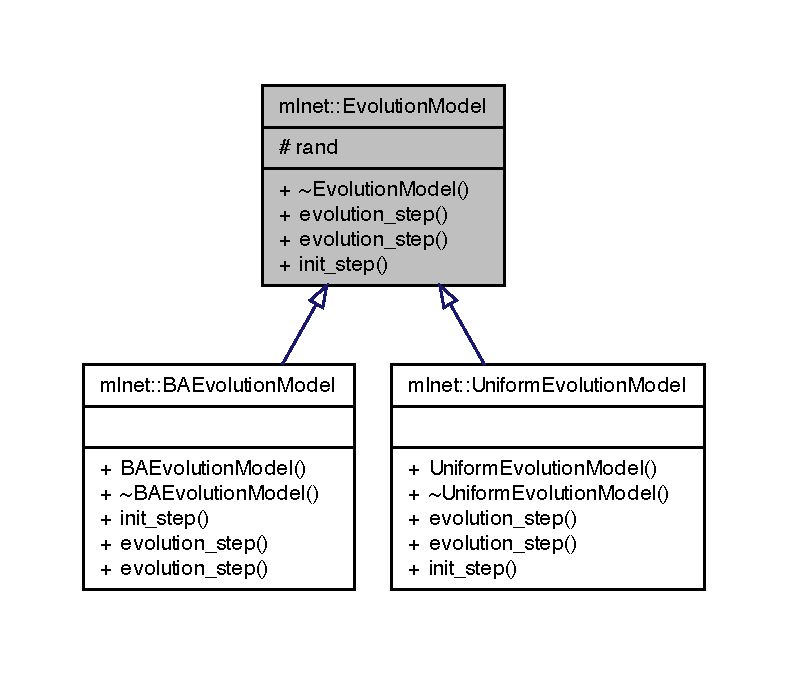
\includegraphics[width=350pt]{classmlnet_1_1_evolution_model__inherit__graph}
\end{center}
\end{figure}


Collaboration diagram for mlnet\+:\+:Evolution\+Model\+:\nopagebreak
\begin{figure}[H]
\begin{center}
\leavevmode
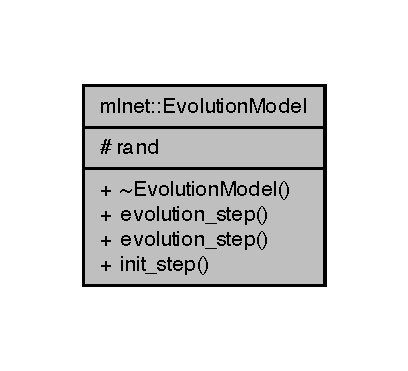
\includegraphics[width=196pt]{classmlnet_1_1_evolution_model__coll__graph}
\end{center}
\end{figure}
\subsection*{Public Member Functions}
\begin{DoxyCompactItemize}
\item 
\hypertarget{classmlnet_1_1_evolution_model_ac4ee4d547e21c3ce4dbe0b721b69999d}{virtual void {\bfseries evolution\+\_\+step} (\hyperlink{classmlnet_1_1_m_l_network}{M\+L\+Network} \&mnet, \hyperlink{namespacemlnet_a84ad9c6056f0eb7d129995351f9b13fb}{layer\+\_\+id} net)=0}\label{classmlnet_1_1_evolution_model_ac4ee4d547e21c3ce4dbe0b721b69999d}

\item 
\hypertarget{classmlnet_1_1_evolution_model_a784021db951c97adbbf679b02d7466de}{virtual void {\bfseries evolution\+\_\+step} (\hyperlink{classmlnet_1_1_m_l_network}{M\+L\+Network} \&mnet, \hyperlink{namespacemlnet_a84ad9c6056f0eb7d129995351f9b13fb}{layer\+\_\+id} net, std\+::set$<$ \hyperlink{namespacemlnet_a4c354f08ca868982bf3ddae882ff71c6}{node\+\_\+id} $>$ \&new\+\_\+vertexes, std\+::set$<$ \hyperlink{namespacemlnet_ad708e58e72680351e102e6b3d0489145}{edge\+\_\+id} $>$ \&new\+\_\+edges)=0}\label{classmlnet_1_1_evolution_model_a784021db951c97adbbf679b02d7466de}

\item 
\hypertarget{classmlnet_1_1_evolution_model_a6ebe6005b628535025819d52eee12f02}{virtual void {\bfseries init\+\_\+step} (\hyperlink{classmlnet_1_1_m_l_network}{M\+L\+Network} \&mnet, \hyperlink{namespacemlnet_a84ad9c6056f0eb7d129995351f9b13fb}{layer\+\_\+id} net)=0}\label{classmlnet_1_1_evolution_model_a6ebe6005b628535025819d52eee12f02}

\end{DoxyCompactItemize}
\subsection*{Protected Attributes}
\begin{DoxyCompactItemize}
\item 
\hypertarget{classmlnet_1_1_evolution_model_a634df31faea6dfe62dd2c9d3ea150b22}{Random {\bfseries rand}}\label{classmlnet_1_1_evolution_model_a634df31faea6dfe62dd2c9d3ea150b22}

\end{DoxyCompactItemize}


\subsection{Detailed Description}
Evolution models 

The documentation for this class was generated from the following file\+:\begin{DoxyCompactItemize}
\item 
include/evolution.\+h\end{DoxyCompactItemize}

\hypertarget{class_file_not_found_exception}{\section{File\+Not\+Found\+Exception Class Reference}
\label{class_file_not_found_exception}\index{File\+Not\+Found\+Exception@{File\+Not\+Found\+Exception}}
}


Inheritance diagram for File\+Not\+Found\+Exception\+:\nopagebreak
\begin{figure}[H]
\begin{center}
\leavevmode
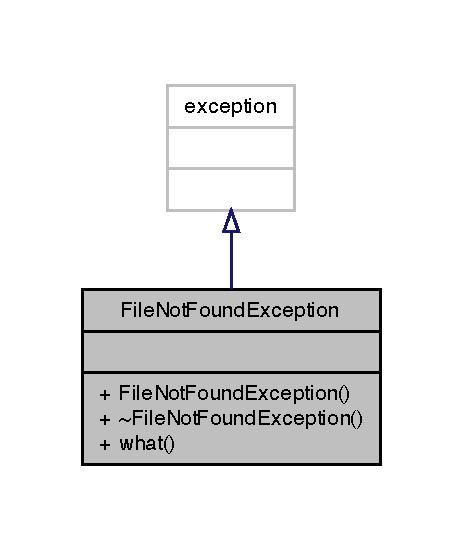
\includegraphics[width=222pt]{class_file_not_found_exception__inherit__graph}
\end{center}
\end{figure}


Collaboration diagram for File\+Not\+Found\+Exception\+:\nopagebreak
\begin{figure}[H]
\begin{center}
\leavevmode
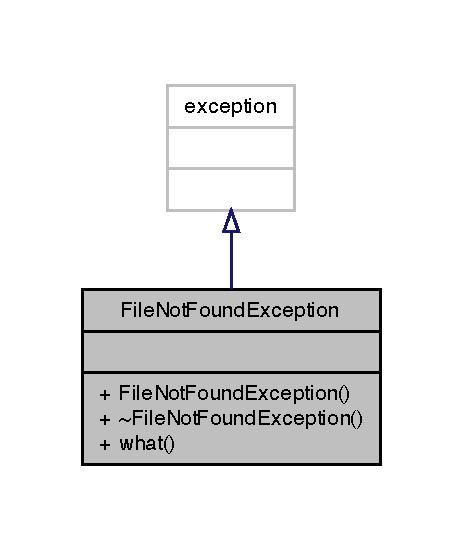
\includegraphics[width=222pt]{class_file_not_found_exception__coll__graph}
\end{center}
\end{figure}
\subsection*{Public Member Functions}
\begin{DoxyCompactItemize}
\item 
\hypertarget{class_file_not_found_exception_a448e085ea8a1fd74ed8cec2cba4c4c37}{{\bfseries File\+Not\+Found\+Exception} (std\+::string path)}\label{class_file_not_found_exception_a448e085ea8a1fd74ed8cec2cba4c4c37}

\item 
\hypertarget{class_file_not_found_exception_a65fad87ab27df5213e8494a19b7a8048}{virtual const char $\ast$ {\bfseries what} () const   throw ()}\label{class_file_not_found_exception_a65fad87ab27df5213e8494a19b7a8048}

\end{DoxyCompactItemize}


The documentation for this class was generated from the following file\+:\begin{DoxyCompactItemize}
\item 
include/exceptions.\+h\end{DoxyCompactItemize}

\hypertarget{classmlnet_1_1_sorted_set_1_1iterator}{\section{mlnet\+:\+:Sorted\+Set$<$ T $>$\+:\+:iterator Class Reference}
\label{classmlnet_1_1_sorted_set_1_1iterator}\index{mlnet\+::\+Sorted\+Set$<$ T $>$\+::iterator@{mlnet\+::\+Sorted\+Set$<$ T $>$\+::iterator}}
}


{\ttfamily \#include $<$datastructures.\+h$>$}



Collaboration diagram for mlnet\+:\+:Sorted\+Set$<$ T $>$\+:\+:iterator\+:\nopagebreak
\begin{figure}[H]
\begin{center}
\leavevmode
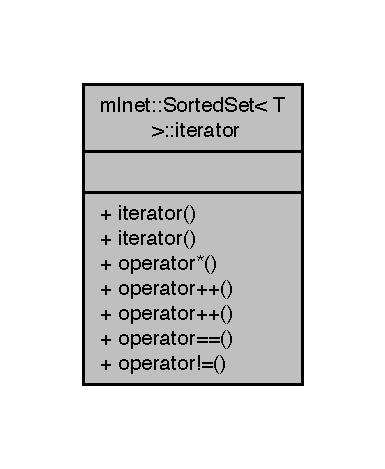
\includegraphics[width=185pt]{classmlnet_1_1_sorted_set_1_1iterator__coll__graph}
\end{center}
\end{figure}
\subsection*{Public Member Functions}
\begin{DoxyCompactItemize}
\item 
\hyperlink{classmlnet_1_1_sorted_set_1_1iterator_abfc1ad310ea30a6e0f9b0566536b81a6}{iterator} (\hyperlink{classmlnet_1_1_entry}{Entry}$<$ T $>$ $\ast$iter)
\item 
T \hyperlink{classmlnet_1_1_sorted_set_1_1iterator_a89f04d3d89bd68deca3d479d144ecd65}{operator$\ast$} ()
\item 
\hyperlink{classmlnet_1_1_sorted_set_1_1iterator}{iterator} \hyperlink{classmlnet_1_1_sorted_set_1_1iterator_a6ab754a90c99638e29a3c2d50c038a89}{operator++} ()
\item 
\hyperlink{classmlnet_1_1_sorted_set_1_1iterator}{iterator} \hyperlink{classmlnet_1_1_sorted_set_1_1iterator_a95afe4bf10cd2f15c144a452803bd41c}{operator++} (int)
\item 
bool \hyperlink{classmlnet_1_1_sorted_set_1_1iterator_ac09be91863ffe86b2971ea099bbe3779}{operator==} (const \hyperlink{classmlnet_1_1_sorted_set}{Sorted\+Set}$<$ T $>$\+::\hyperlink{classmlnet_1_1_sorted_set_1_1iterator}{iterator} \&rhs)
\item 
bool \hyperlink{classmlnet_1_1_sorted_set_1_1iterator_aca02d0e9e432005af28e090cebe20716}{operator!=} (const \hyperlink{classmlnet_1_1_sorted_set}{Sorted\+Set}$<$ T $>$\+::\hyperlink{classmlnet_1_1_sorted_set_1_1iterator}{iterator} \&rhs)
\end{DoxyCompactItemize}


\subsection{Detailed Description}
\subsubsection*{template$<$class T$>$class mlnet\+::\+Sorted\+Set$<$ T $>$\+::iterator}

Iterator over the obects in this collection 

\subsection{Constructor \& Destructor Documentation}
\hypertarget{classmlnet_1_1_sorted_set_1_1iterator_abfc1ad310ea30a6e0f9b0566536b81a6}{\index{mlnet\+::\+Sorted\+Set\+::iterator@{mlnet\+::\+Sorted\+Set\+::iterator}!iterator@{iterator}}
\index{iterator@{iterator}!mlnet\+::\+Sorted\+Set\+::iterator@{mlnet\+::\+Sorted\+Set\+::iterator}}
\subsubsection[{iterator}]{\setlength{\rightskip}{0pt plus 5cm}template$<$class T$>$ Sorted\+Set\+::iterator\+::iterator (
\begin{DoxyParamCaption}
\item[{{\bf Entry}$<$ T $>$ $\ast$}]{iter}
\end{DoxyParamCaption}
)}}\label{classmlnet_1_1_sorted_set_1_1iterator_abfc1ad310ea30a6e0f9b0566536b81a6}
Returns an iterator pointing at the input object 

\subsection{Member Function Documentation}
\hypertarget{classmlnet_1_1_sorted_set_1_1iterator_aca02d0e9e432005af28e090cebe20716}{\index{mlnet\+::\+Sorted\+Set\+::iterator@{mlnet\+::\+Sorted\+Set\+::iterator}!operator"!=@{operator"!=}}
\index{operator"!=@{operator"!=}!mlnet\+::\+Sorted\+Set\+::iterator@{mlnet\+::\+Sorted\+Set\+::iterator}}
\subsubsection[{operator"!=}]{\setlength{\rightskip}{0pt plus 5cm}template$<$class T$>$ bool Sorted\+Set\+::iterator\+::operator!= (
\begin{DoxyParamCaption}
\item[{const {\bf Sorted\+Set}$<$ T $>$\+::{\bf iterator} \&}]{rhs}
\end{DoxyParamCaption}
)}}\label{classmlnet_1_1_sorted_set_1_1iterator_aca02d0e9e432005af28e090cebe20716}
Checks if this iterator differs from the input one \hypertarget{classmlnet_1_1_sorted_set_1_1iterator_a89f04d3d89bd68deca3d479d144ecd65}{\index{mlnet\+::\+Sorted\+Set\+::iterator@{mlnet\+::\+Sorted\+Set\+::iterator}!operator$\ast$@{operator$\ast$}}
\index{operator$\ast$@{operator$\ast$}!mlnet\+::\+Sorted\+Set\+::iterator@{mlnet\+::\+Sorted\+Set\+::iterator}}
\subsubsection[{operator$\ast$}]{\setlength{\rightskip}{0pt plus 5cm}template$<$class T $>$ T Sorted\+Set\+::iterator\+::operator$\ast$ (
\begin{DoxyParamCaption}
{}
\end{DoxyParamCaption}
)}}\label{classmlnet_1_1_sorted_set_1_1iterator_a89f04d3d89bd68deca3d479d144ecd65}
Return the object pointed by this iterator \hypertarget{classmlnet_1_1_sorted_set_1_1iterator_a6ab754a90c99638e29a3c2d50c038a89}{\index{mlnet\+::\+Sorted\+Set\+::iterator@{mlnet\+::\+Sorted\+Set\+::iterator}!operator++@{operator++}}
\index{operator++@{operator++}!mlnet\+::\+Sorted\+Set\+::iterator@{mlnet\+::\+Sorted\+Set\+::iterator}}
\subsubsection[{operator++}]{\setlength{\rightskip}{0pt plus 5cm}template$<$class T $>$ {\bf Sorted\+Set}$<$ T $>$\+::{\bf iterator} Sorted\+Set\+::iterator\+::operator++ (
\begin{DoxyParamCaption}
{}
\end{DoxyParamCaption}
)}}\label{classmlnet_1_1_sorted_set_1_1iterator_a6ab754a90c99638e29a3c2d50c038a89}
Moves the iterator to the next object in the collection (prefix) \hypertarget{classmlnet_1_1_sorted_set_1_1iterator_a95afe4bf10cd2f15c144a452803bd41c}{\index{mlnet\+::\+Sorted\+Set\+::iterator@{mlnet\+::\+Sorted\+Set\+::iterator}!operator++@{operator++}}
\index{operator++@{operator++}!mlnet\+::\+Sorted\+Set\+::iterator@{mlnet\+::\+Sorted\+Set\+::iterator}}
\subsubsection[{operator++}]{\setlength{\rightskip}{0pt plus 5cm}template$<$class T $>$ {\bf Sorted\+Set}$<$ T $>$\+::{\bf iterator} Sorted\+Set\+::iterator\+::operator++ (
\begin{DoxyParamCaption}
\item[{int}]{}
\end{DoxyParamCaption}
)}}\label{classmlnet_1_1_sorted_set_1_1iterator_a95afe4bf10cd2f15c144a452803bd41c}
Moves the iterator to the next object in the collection (postfix) \hypertarget{classmlnet_1_1_sorted_set_1_1iterator_ac09be91863ffe86b2971ea099bbe3779}{\index{mlnet\+::\+Sorted\+Set\+::iterator@{mlnet\+::\+Sorted\+Set\+::iterator}!operator==@{operator==}}
\index{operator==@{operator==}!mlnet\+::\+Sorted\+Set\+::iterator@{mlnet\+::\+Sorted\+Set\+::iterator}}
\subsubsection[{operator==}]{\setlength{\rightskip}{0pt plus 5cm}template$<$class T$>$ bool Sorted\+Set\+::iterator\+::operator== (
\begin{DoxyParamCaption}
\item[{const {\bf Sorted\+Set}$<$ T $>$\+::{\bf iterator} \&}]{rhs}
\end{DoxyParamCaption}
)}}\label{classmlnet_1_1_sorted_set_1_1iterator_ac09be91863ffe86b2971ea099bbe3779}
Checks if this iterator equals the input one 

The documentation for this class was generated from the following files\+:\begin{DoxyCompactItemize}
\item 
include/datastructures.\+h\item 
include/sortedset.\+cpp\end{DoxyCompactItemize}

\hypertarget{classmlnet_1_1layer}{\section{mlnet\+:\+:layer Class Reference}
\label{classmlnet_1_1layer}\index{mlnet\+::layer@{mlnet\+::layer}}
}


{\ttfamily \#include $<$datastructures.\+h$>$}



Inheritance diagram for mlnet\+:\+:layer\+:\nopagebreak
\begin{figure}[H]
\begin{center}
\leavevmode
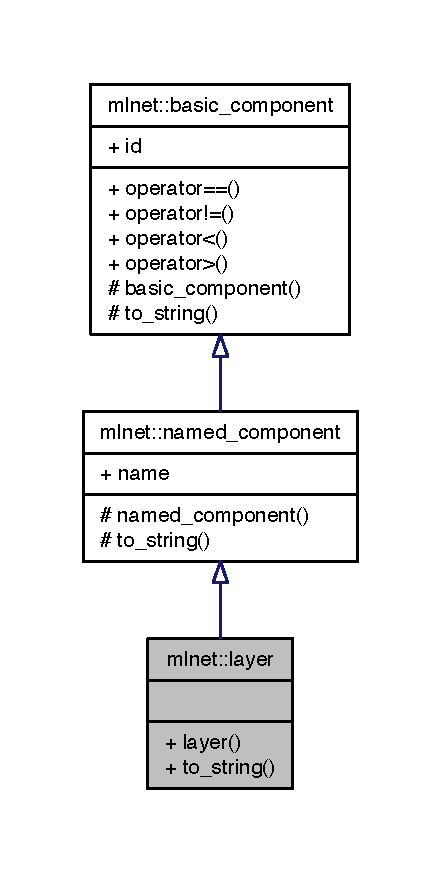
\includegraphics[width=212pt]{classmlnet_1_1layer__inherit__graph}
\end{center}
\end{figure}


Collaboration diagram for mlnet\+:\+:layer\+:\nopagebreak
\begin{figure}[H]
\begin{center}
\leavevmode
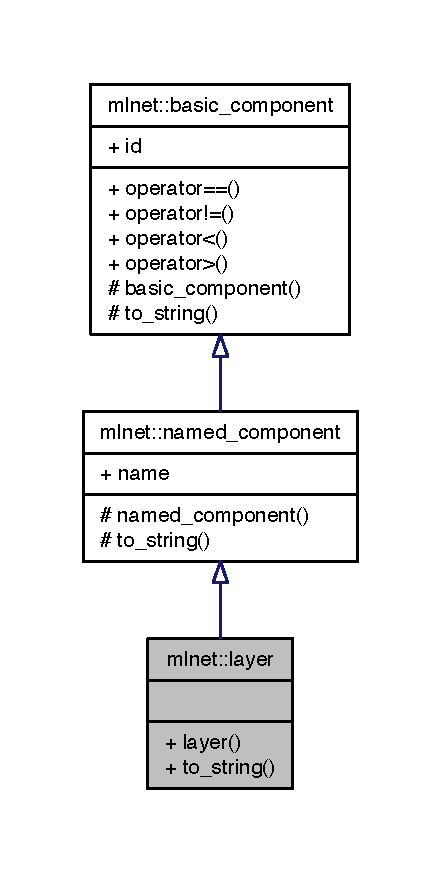
\includegraphics[width=212pt]{classmlnet_1_1layer__coll__graph}
\end{center}
\end{figure}
\subsection*{Public Member Functions}
\begin{DoxyCompactItemize}
\item 
\hyperlink{classmlnet_1_1layer_a4b3b77912bdb71f481028174e22f5a25}{layer} (const \hyperlink{namespacemlnet_a84ad9c6056f0eb7d129995351f9b13fb}{layer\+\_\+id} \&\hyperlink{classmlnet_1_1basic__component_a7d56ea959ef686405bc0fa4830b03347}{id}, const std\+::string \&\hyperlink{classmlnet_1_1named__component_a3015f6650729352abae8fb01e7ee7ca7}{name})
\item 
std\+::string \hyperlink{classmlnet_1_1layer_a3a7efb6528fc88b0e093957c66830bd5}{to\+\_\+string} () const 
\end{DoxyCompactItemize}
\subsection*{Additional Inherited Members}


\subsection{Detailed Description}
A layer in a \hyperlink{classmlnet_1_1_m_l_network}{M\+L\+Network}. 

\subsection{Constructor \& Destructor Documentation}
\hypertarget{classmlnet_1_1layer_a4b3b77912bdb71f481028174e22f5a25}{\index{mlnet\+::layer@{mlnet\+::layer}!layer@{layer}}
\index{layer@{layer}!mlnet\+::layer@{mlnet\+::layer}}
\subsubsection[{layer}]{\setlength{\rightskip}{0pt plus 5cm}mlnet\+::layer\+::layer (
\begin{DoxyParamCaption}
\item[{const {\bf layer\+\_\+id} \&}]{id, }
\item[{const std\+::string \&}]{name}
\end{DoxyParamCaption}
)}}\label{classmlnet_1_1layer_a4b3b77912bdb71f481028174e22f5a25}
Constructor 

\subsection{Member Function Documentation}
\hypertarget{classmlnet_1_1layer_a3a7efb6528fc88b0e093957c66830bd5}{\index{mlnet\+::layer@{mlnet\+::layer}!to\+\_\+string@{to\+\_\+string}}
\index{to\+\_\+string@{to\+\_\+string}!mlnet\+::layer@{mlnet\+::layer}}
\subsubsection[{to\+\_\+string}]{\setlength{\rightskip}{0pt plus 5cm}std\+::string mlnet\+::layer\+::to\+\_\+string (
\begin{DoxyParamCaption}
{}
\end{DoxyParamCaption}
) const}}\label{classmlnet_1_1layer_a3a7efb6528fc88b0e093957c66830bd5}
Output function, presenting a complete description of the layer 

The documentation for this class was generated from the following file\+:\begin{DoxyCompactItemize}
\item 
include/datastructures.\+h\end{DoxyCompactItemize}

\hypertarget{classmlnet_1_1_m_l_network}{\section{mlnet\+:\+:M\+L\+Network Class Reference}
\label{classmlnet_1_1_m_l_network}\index{mlnet\+::\+M\+L\+Network@{mlnet\+::\+M\+L\+Network}}
}


{\ttfamily \#include $<$datastructures.\+h$>$}



Collaboration diagram for mlnet\+:\+:M\+L\+Network\+:\nopagebreak
\begin{figure}[H]
\begin{center}
\leavevmode
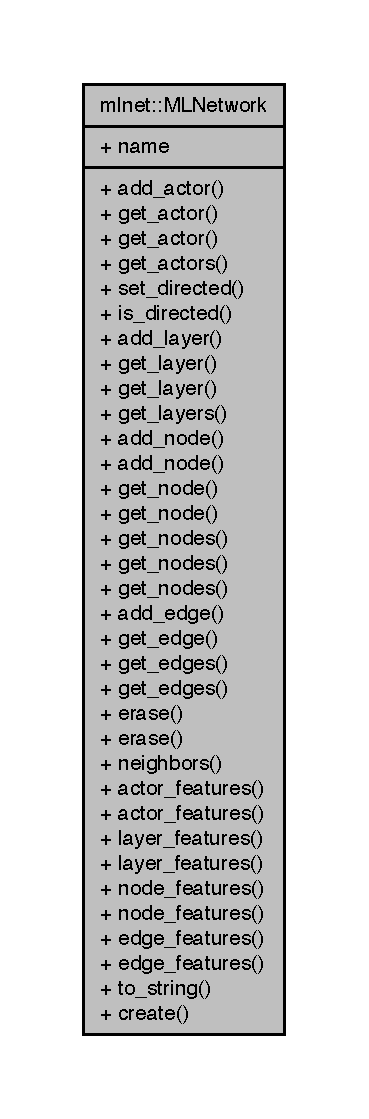
\includegraphics[width=177pt]{classmlnet_1_1_m_l_network__coll__graph}
\end{center}
\end{figure}
\subsection*{Public Member Functions}
\begin{DoxyCompactItemize}
\item 
\hyperlink{namespacemlnet_a714fd98ffaeaadd5c38d61fa53dc4d24}{Actor\+Shared\+Ptr} \hyperlink{classmlnet_1_1_m_l_network_aaf56134e14342a301a0d13fcf446b1c4}{add\+\_\+actor} (const std\+::string \&\hyperlink{classmlnet_1_1_m_l_network_aa2e1496321423e15a8e97e0daed30ca7}{name})
\begin{DoxyCompactList}\small\item\em Adds a new actor to the \hyperlink{classmlnet_1_1_m_l_network}{M\+L\+Network}. A new identifier is automatically associated to the new actor. \end{DoxyCompactList}\item 
\hyperlink{namespacemlnet_a714fd98ffaeaadd5c38d61fa53dc4d24}{Actor\+Shared\+Ptr} \hyperlink{classmlnet_1_1_m_l_network_a28d2ad6ba24d565fd4e0fb3ddeb90659}{get\+\_\+actor} (const \hyperlink{namespacemlnet_a1d557bff46b627f1d7f6ff613302bba5}{actor\+\_\+id} \&id) const 
\begin{DoxyCompactList}\small\item\em Returns an actor by I\+D. This method can also be used to check if an actor is present in the \hyperlink{classmlnet_1_1_m_l_network}{M\+L\+Network}. \end{DoxyCompactList}\item 
\hyperlink{namespacemlnet_a714fd98ffaeaadd5c38d61fa53dc4d24}{Actor\+Shared\+Ptr} \hyperlink{classmlnet_1_1_m_l_network_a4031cb1bc3b5de9a204394b38fbfd321}{get\+\_\+actor} (const std\+::string \&\hyperlink{classmlnet_1_1_m_l_network_aa2e1496321423e15a8e97e0daed30ca7}{name}) const 
\begin{DoxyCompactList}\small\item\em Returns an actor by name. This function can also be used to check if an actor is present in the \hyperlink{classmlnet_1_1_m_l_network}{M\+L\+Network}. \end{DoxyCompactList}\item 
const \hyperlink{classmlnet_1_1_sorted_set}{Sorted\+Set}$<$ \hyperlink{namespacemlnet_a714fd98ffaeaadd5c38d61fa53dc4d24}{Actor\+Shared\+Ptr} $>$ \& \hyperlink{classmlnet_1_1_m_l_network_a730f339a39be9b95b1c0ec6e029cabf1}{get\+\_\+actors} () const 
\begin{DoxyCompactList}\small\item\em Returns all the actors in the \hyperlink{classmlnet_1_1_m_l_network}{M\+L\+Network}. \end{DoxyCompactList}\item 
void \hyperlink{classmlnet_1_1_m_l_network_a17c4df943b713597c191bdad8a844fb5}{set\+\_\+directed} (\hyperlink{namespacemlnet_a10c007fb811c55339dd5b9d32bb0505d}{Layer\+Shared\+Ptr} layer1, \hyperlink{namespacemlnet_a10c007fb811c55339dd5b9d32bb0505d}{Layer\+Shared\+Ptr} layer2, bool directed)
\begin{DoxyCompactList}\small\item\em Sets the default edge directionality depending on the layers of the connected nodes. \end{DoxyCompactList}\item 
bool \hyperlink{classmlnet_1_1_m_l_network_ac7e339d6c2d18acd1adef418346a8888}{is\+\_\+directed} (\hyperlink{namespacemlnet_a10c007fb811c55339dd5b9d32bb0505d}{Layer\+Shared\+Ptr} layer1, \hyperlink{namespacemlnet_a10c007fb811c55339dd5b9d32bb0505d}{Layer\+Shared\+Ptr} layer2) const 
\begin{DoxyCompactList}\small\item\em Gets the default edge directionality depending on the layers of the connected nodes. \end{DoxyCompactList}\item 
\hyperlink{namespacemlnet_a10c007fb811c55339dd5b9d32bb0505d}{Layer\+Shared\+Ptr} \hyperlink{classmlnet_1_1_m_l_network_a5ee8b4d3dbce2b4f581c2b3328ec3968}{add\+\_\+layer} (const std\+::string \&\hyperlink{classmlnet_1_1_m_l_network_aa2e1496321423e15a8e97e0daed30ca7}{name}, bool directed)
\begin{DoxyCompactList}\small\item\em Adds a new layer to the \hyperlink{classmlnet_1_1_m_l_network}{M\+L\+Network}. A new identifier is automatically associated to the new layer. \end{DoxyCompactList}\item 
\hyperlink{namespacemlnet_a10c007fb811c55339dd5b9d32bb0505d}{Layer\+Shared\+Ptr} \hyperlink{classmlnet_1_1_m_l_network_a1bfb2989c14ac0dbfa836de5c3ae94cf}{get\+\_\+layer} (const \hyperlink{namespacemlnet_a84ad9c6056f0eb7d129995351f9b13fb}{layer\+\_\+id} \&id) const 
\begin{DoxyCompactList}\small\item\em Returns a layer by I\+D. This function can also be used to check if a layer is present in the \hyperlink{classmlnet_1_1_m_l_network}{M\+L\+Network}. \end{DoxyCompactList}\item 
\hyperlink{namespacemlnet_a10c007fb811c55339dd5b9d32bb0505d}{Layer\+Shared\+Ptr} \hyperlink{classmlnet_1_1_m_l_network_a788bb8d8f559e76deb6c14b58b15bb82}{get\+\_\+layer} (const std\+::string \&\hyperlink{classmlnet_1_1_m_l_network_aa2e1496321423e15a8e97e0daed30ca7}{name}) const 
\begin{DoxyCompactList}\small\item\em Returns a layer by name. This function can also be used to check if a layer is present in the \hyperlink{classmlnet_1_1_m_l_network}{M\+L\+Network}. \end{DoxyCompactList}\item 
const \hyperlink{classmlnet_1_1_sorted_set}{Sorted\+Set}$<$ \hyperlink{namespacemlnet_a10c007fb811c55339dd5b9d32bb0505d}{Layer\+Shared\+Ptr} $>$ \& \hyperlink{classmlnet_1_1_m_l_network_a1ff6d760dd7aabdcf889c30107025354}{get\+\_\+layers} () const 
\begin{DoxyCompactList}\small\item\em Returns all the layers in the \hyperlink{classmlnet_1_1_m_l_network}{M\+L\+Network}. \end{DoxyCompactList}\item 
\hyperlink{namespacemlnet_acf8b1b6deb52e7dacfc676c689f9a10c}{Node\+Shared\+Ptr} \hyperlink{classmlnet_1_1_m_l_network_a4ee0a93e953d9807f3db3ee70a475faf}{add\+\_\+node} (const \hyperlink{namespacemlnet_a714fd98ffaeaadd5c38d61fa53dc4d24}{Actor\+Shared\+Ptr} \&\hyperlink{classmlnet_1_1actor}{actor}, const \hyperlink{namespacemlnet_a10c007fb811c55339dd5b9d32bb0505d}{Layer\+Shared\+Ptr} \&\hyperlink{classmlnet_1_1layer}{layer})
\begin{DoxyCompactList}\small\item\em Adds a new node to the \hyperlink{classmlnet_1_1_m_l_network}{M\+L\+Network}. A new identifier and a default name are automatically associated to the new node. \end{DoxyCompactList}\item 
\hyperlink{namespacemlnet_acf8b1b6deb52e7dacfc676c689f9a10c}{Node\+Shared\+Ptr} \hyperlink{classmlnet_1_1_m_l_network_ad39a45f153b4dc69f6585d1fcd39ab3f}{add\+\_\+node} (const std\+::string \&\hyperlink{classmlnet_1_1_m_l_network_aa2e1496321423e15a8e97e0daed30ca7}{name}, const \hyperlink{namespacemlnet_a714fd98ffaeaadd5c38d61fa53dc4d24}{Actor\+Shared\+Ptr} \&\hyperlink{classmlnet_1_1actor}{actor}, const \hyperlink{namespacemlnet_a10c007fb811c55339dd5b9d32bb0505d}{Layer\+Shared\+Ptr} \&\hyperlink{classmlnet_1_1layer}{layer})
\begin{DoxyCompactList}\small\item\em Adds a new node to the \hyperlink{classmlnet_1_1_m_l_network}{M\+L\+Network}. A new identifier is automatically associated to the new node. \end{DoxyCompactList}\item 
\hyperlink{namespacemlnet_acf8b1b6deb52e7dacfc676c689f9a10c}{Node\+Shared\+Ptr} \hyperlink{classmlnet_1_1_m_l_network_abc3494cf0f75b871a619cee338bdf86f}{get\+\_\+node} (const \hyperlink{namespacemlnet_a4c354f08ca868982bf3ddae882ff71c6}{node\+\_\+id} \&id) const 
\begin{DoxyCompactList}\small\item\em Returns a node by I\+D. This function can also be used to check if a node is present in the \hyperlink{classmlnet_1_1_m_l_network}{M\+L\+Network}. \end{DoxyCompactList}\item 
\hyperlink{namespacemlnet_acf8b1b6deb52e7dacfc676c689f9a10c}{Node\+Shared\+Ptr} \hyperlink{classmlnet_1_1_m_l_network_af92d95a75d66e665cd689e9666f30206}{get\+\_\+node} (const \hyperlink{namespacemlnet_a714fd98ffaeaadd5c38d61fa53dc4d24}{Actor\+Shared\+Ptr} \&\hyperlink{classmlnet_1_1actor}{actor}, const \hyperlink{namespacemlnet_a10c007fb811c55339dd5b9d32bb0505d}{Layer\+Shared\+Ptr} \&\hyperlink{classmlnet_1_1layer}{layer}) const 
\begin{DoxyCompactList}\small\item\em Returns a node by specifying an actor and a layer. This function can also be used to check if a node is present in the \hyperlink{classmlnet_1_1_m_l_network}{M\+L\+Network}. \end{DoxyCompactList}\item 
const \hyperlink{classmlnet_1_1_sorted_set}{Sorted\+Set}$<$ \hyperlink{namespacemlnet_acf8b1b6deb52e7dacfc676c689f9a10c}{Node\+Shared\+Ptr} $>$ \& \hyperlink{classmlnet_1_1_m_l_network_afa99d24cafa9095887cb457c2a853924}{get\+\_\+nodes} () const 
\begin{DoxyCompactList}\small\item\em Returns all the nodes in the \hyperlink{classmlnet_1_1_m_l_network}{M\+L\+Network}. \end{DoxyCompactList}\item 
const \hyperlink{classmlnet_1_1_sorted_set}{Sorted\+Set}$<$ \hyperlink{namespacemlnet_acf8b1b6deb52e7dacfc676c689f9a10c}{Node\+Shared\+Ptr} $>$ \& \hyperlink{classmlnet_1_1_m_l_network_a19d12194812eafe8b3ab6c75ed13c1c2}{get\+\_\+nodes} (const \hyperlink{namespacemlnet_a10c007fb811c55339dd5b9d32bb0505d}{Layer\+Shared\+Ptr} \&\hyperlink{classmlnet_1_1layer}{layer}) const 
\begin{DoxyCompactList}\small\item\em Returns all the nodes in a layer. \end{DoxyCompactList}\item 
const \hyperlink{classmlnet_1_1_sorted_set}{Sorted\+Set}$<$ \hyperlink{namespacemlnet_acf8b1b6deb52e7dacfc676c689f9a10c}{Node\+Shared\+Ptr} $>$ \& \hyperlink{classmlnet_1_1_m_l_network_a9c62dc703796e78a2bad9959fcfd9632}{get\+\_\+nodes} (const \hyperlink{namespacemlnet_a714fd98ffaeaadd5c38d61fa53dc4d24}{Actor\+Shared\+Ptr} \&\hyperlink{classmlnet_1_1actor}{actor}) const 
\begin{DoxyCompactList}\small\item\em Returns the nodes associated to the input actor. \end{DoxyCompactList}\item 
\hyperlink{namespacemlnet_a33e88c3df9bea691a269d5e5d8bea57d}{Edge\+Shared\+Ptr} \hyperlink{classmlnet_1_1_m_l_network_a41360f23aedbece293900ab0098348cd}{add\+\_\+edge} (const \hyperlink{namespacemlnet_acf8b1b6deb52e7dacfc676c689f9a10c}{Node\+Shared\+Ptr} \&node1, const \hyperlink{namespacemlnet_acf8b1b6deb52e7dacfc676c689f9a10c}{Node\+Shared\+Ptr} \&node2)
\begin{DoxyCompactList}\small\item\em Adds a new edge to the \hyperlink{classmlnet_1_1_m_l_network}{M\+L\+Network}. Multiple edges between the same pair of nodes are not allowed. The directionality of the edge is defined by the layers of the two nodes. \end{DoxyCompactList}\item 
\hyperlink{namespacemlnet_a33e88c3df9bea691a269d5e5d8bea57d}{Edge\+Shared\+Ptr} \hyperlink{classmlnet_1_1_m_l_network_ad122937d266e66e75d47b2c43ccfe35b}{get\+\_\+edge} (const \hyperlink{namespacemlnet_acf8b1b6deb52e7dacfc676c689f9a10c}{Node\+Shared\+Ptr} \&node1, const \hyperlink{namespacemlnet_acf8b1b6deb52e7dacfc676c689f9a10c}{Node\+Shared\+Ptr} \&node2) const 
\begin{DoxyCompactList}\small\item\em Returns an edge. This function can also be used to check if an edge is present in the \hyperlink{classmlnet_1_1_m_l_network}{M\+L\+Network}. \end{DoxyCompactList}\item 
const \hyperlink{classmlnet_1_1_sorted_set}{Sorted\+Set}$<$ \hyperlink{namespacemlnet_a33e88c3df9bea691a269d5e5d8bea57d}{Edge\+Shared\+Ptr} $>$ \& \hyperlink{classmlnet_1_1_m_l_network_af2b8de761af4708080e24f1444518c59}{get\+\_\+edges} () const 
\begin{DoxyCompactList}\small\item\em Returns all the edges in the \hyperlink{classmlnet_1_1_m_l_network}{M\+L\+Network}. \end{DoxyCompactList}\item 
const \hyperlink{classmlnet_1_1_sorted_set}{Sorted\+Set}$<$ \hyperlink{namespacemlnet_a33e88c3df9bea691a269d5e5d8bea57d}{Edge\+Shared\+Ptr} $>$ \& \hyperlink{classmlnet_1_1_m_l_network_a0e74f242ffc76837a3789f2e3e7a47be}{get\+\_\+edges} (const \hyperlink{namespacemlnet_a10c007fb811c55339dd5b9d32bb0505d}{Layer\+Shared\+Ptr} \&layer1, const \hyperlink{namespacemlnet_a10c007fb811c55339dd5b9d32bb0505d}{Layer\+Shared\+Ptr} \&layer2) const 
\begin{DoxyCompactList}\small\item\em Returns all the edges from a layer A to a layer B. This method can also retrieve intra-\/layer edges setting A = B. \end{DoxyCompactList}\item 
void \hyperlink{classmlnet_1_1_m_l_network_a071867d31c8c24a5f209af1c3b84aeeb}{erase} (const \hyperlink{namespacemlnet_acf8b1b6deb52e7dacfc676c689f9a10c}{Node\+Shared\+Ptr} \&\hyperlink{classmlnet_1_1node}{node})
\begin{DoxyCompactList}\small\item\em Deletes an existing node. All related data, including node attributes and edges involving this node, are also deleted. \end{DoxyCompactList}\item 
void \hyperlink{classmlnet_1_1_m_l_network_a4767b97853e3a9e248e2cedeaa64e3d0}{erase} (const \hyperlink{namespacemlnet_a33e88c3df9bea691a269d5e5d8bea57d}{Edge\+Shared\+Ptr} \&\hyperlink{classmlnet_1_1edge}{edge})
\begin{DoxyCompactList}\small\item\em Deletes an existing edge. \hyperlink{classmlnet_1_1_attribute}{Attribute} values associated to this edge are also deleted. \end{DoxyCompactList}\item 
const \hyperlink{classmlnet_1_1_sorted_set}{Sorted\+Set}$<$ \hyperlink{namespacemlnet_acf8b1b6deb52e7dacfc676c689f9a10c}{Node\+Shared\+Ptr} $>$ \& \hyperlink{classmlnet_1_1_m_l_network_aa81b9028f4f183857ac8c7939cb4fc39}{neighbors} (const \hyperlink{namespacemlnet_acf8b1b6deb52e7dacfc676c689f9a10c}{Node\+Shared\+Ptr} \&\hyperlink{classmlnet_1_1node}{node}, int mode) const 
\begin{DoxyCompactList}\small\item\em Returns the nodes with an edge from/to the input node. \end{DoxyCompactList}\item 
\hyperlink{namespacemlnet_a3d60b9ef6ef6489d000f6061e0a1bdf2}{Attribute\+Store\+Shared\+Ptr} \hyperlink{classmlnet_1_1_m_l_network_a4367cd80f2528c72acbaaed91de62b8b}{actor\+\_\+features} ()
\begin{DoxyCompactList}\small\item\em Allows the manipulation of feature vectors associated to actors. This function is not thread-\/safe. \end{DoxyCompactList}\item 
const \hyperlink{namespacemlnet_a3d60b9ef6ef6489d000f6061e0a1bdf2}{Attribute\+Store\+Shared\+Ptr} \hyperlink{classmlnet_1_1_m_l_network_a6bb89ed6554e96acd80ba8126dd0afa8}{actor\+\_\+features} () const 
\begin{DoxyCompactList}\small\item\em Allows the inspection of feature vectors associated to actors. This function is not thread-\/safe. \end{DoxyCompactList}\item 
\hyperlink{namespacemlnet_a3d60b9ef6ef6489d000f6061e0a1bdf2}{Attribute\+Store\+Shared\+Ptr} \hyperlink{classmlnet_1_1_m_l_network_a4ee8a60c348feed04577ae8c9060edf8}{layer\+\_\+features} ()
\begin{DoxyCompactList}\small\item\em Allows the manipulation of feature vectors associated to layers. This function is not thread-\/safe. \end{DoxyCompactList}\item 
const \hyperlink{namespacemlnet_a3d60b9ef6ef6489d000f6061e0a1bdf2}{Attribute\+Store\+Shared\+Ptr} \hyperlink{classmlnet_1_1_m_l_network_aa9074cba205ceabc3c0f39a340716935}{layer\+\_\+features} () const 
\begin{DoxyCompactList}\small\item\em Allows the inspection of feature vectors associated to layers. This function is not thread-\/safe. \end{DoxyCompactList}\item 
\hyperlink{namespacemlnet_a3d60b9ef6ef6489d000f6061e0a1bdf2}{Attribute\+Store\+Shared\+Ptr} \hyperlink{classmlnet_1_1_m_l_network_aac41608b673450acca904619cc77d9b2}{node\+\_\+features} (const \hyperlink{namespacemlnet_a10c007fb811c55339dd5b9d32bb0505d}{Layer\+Shared\+Ptr} \&\hyperlink{classmlnet_1_1layer}{layer})
\begin{DoxyCompactList}\small\item\em Allows the manipulation of feature vectors associated to nodes. Every layer can associate different features to its nodes, but all nodes in the same layer have the same features This function is not thread-\/safe. \end{DoxyCompactList}\item 
const \hyperlink{namespacemlnet_a3d60b9ef6ef6489d000f6061e0a1bdf2}{Attribute\+Store\+Shared\+Ptr} \hyperlink{classmlnet_1_1_m_l_network_ab7b28f55476dd9209383ab68d40ff44e}{node\+\_\+features} (const \hyperlink{namespacemlnet_a10c007fb811c55339dd5b9d32bb0505d}{Layer\+Shared\+Ptr} \&\hyperlink{classmlnet_1_1layer}{layer}) const 
\begin{DoxyCompactList}\small\item\em Allows the manipulation of feature vectors associated to nodes. Every layer can associate different features to its nodes, but all nodes in the same layer have the same features This function is not thread-\/safe. \end{DoxyCompactList}\item 
\hyperlink{namespacemlnet_a3d60b9ef6ef6489d000f6061e0a1bdf2}{Attribute\+Store\+Shared\+Ptr} \hyperlink{classmlnet_1_1_m_l_network_a7a72f3e23c9a098fda3e7ef0947f4db9}{edge\+\_\+features} (const \hyperlink{namespacemlnet_a10c007fb811c55339dd5b9d32bb0505d}{Layer\+Shared\+Ptr} \&layer1, const \hyperlink{namespacemlnet_a10c007fb811c55339dd5b9d32bb0505d}{Layer\+Shared\+Ptr} \&layer2)
\begin{DoxyCompactList}\small\item\em Allows the manipulation of feature vectors associated to edges. Every pair of layers corresponds to different edge features, but all edges between the same pair of layers have the same features This function is not thread-\/safe. \end{DoxyCompactList}\item 
const \hyperlink{namespacemlnet_a3d60b9ef6ef6489d000f6061e0a1bdf2}{Attribute\+Store\+Shared\+Ptr} \hyperlink{classmlnet_1_1_m_l_network_acf22ca4a335edf9a68f8304cfb681dcf}{edge\+\_\+features} (const \hyperlink{namespacemlnet_a10c007fb811c55339dd5b9d32bb0505d}{Layer\+Shared\+Ptr} \&layer1, const \hyperlink{namespacemlnet_a10c007fb811c55339dd5b9d32bb0505d}{Layer\+Shared\+Ptr} \&layer2) const 
\begin{DoxyCompactList}\small\item\em Allows the inspection of feature vectors associated to edges. Every pair of layers corresponds to different edge features, but all edges between the same pair of layers have the same features This function is not thread-\/safe. \end{DoxyCompactList}\item 
std\+::string \hyperlink{classmlnet_1_1_m_l_network_aad18a3068440db5d63b4e621749f8812}{to\+\_\+string} () const 
\end{DoxyCompactItemize}
\subsection*{Static Public Member Functions}
\begin{DoxyCompactItemize}
\item 
static \hyperlink{namespacemlnet_aa6d3fa87865bcde4d1283abb1942cbbb}{M\+L\+Network\+Shared\+Ptr} \hyperlink{classmlnet_1_1_m_l_network_af4f8d98426a76652f1a4503c202e3c98}{create} (const std\+::string \&\hyperlink{classmlnet_1_1_m_l_network_aa2e1496321423e15a8e97e0daed30ca7}{name})
\end{DoxyCompactItemize}
\subsection*{Public Attributes}
\begin{DoxyCompactItemize}
\item 
const std\+::string \hyperlink{classmlnet_1_1_m_l_network_aa2e1496321423e15a8e97e0daed30ca7}{name}
\end{DoxyCompactItemize}
\subsection*{Friends}
\begin{DoxyCompactItemize}
\item 
\hypertarget{classmlnet_1_1_m_l_network_adf12125ac9f1f53844917c917c80873e}{class {\bfseries actor\+\_\+list}}\label{classmlnet_1_1_m_l_network_adf12125ac9f1f53844917c917c80873e}

\item 
\hypertarget{classmlnet_1_1_m_l_network_a0b92bd721386a2a578989d4a0876767f}{class {\bfseries layer\+\_\+list}}\label{classmlnet_1_1_m_l_network_a0b92bd721386a2a578989d4a0876767f}

\item 
\hypertarget{classmlnet_1_1_m_l_network_a1b7f8553ab7e425c0d59e59e4399f475}{class {\bfseries node\+\_\+list}}\label{classmlnet_1_1_m_l_network_a1b7f8553ab7e425c0d59e59e4399f475}

\item 
\hypertarget{classmlnet_1_1_m_l_network_ad40e7612c45d00b231b57e69f1b1ff4f}{class {\bfseries edge\+\_\+list}}\label{classmlnet_1_1_m_l_network_ad40e7612c45d00b231b57e69f1b1ff4f}

\end{DoxyCompactItemize}


\subsection{Detailed Description}
\hyperlink{classmlnet_1_1_m_l_network}{M\+L\+Network} Main data structure of the package, defining a multilayer network. 

\subsection{Member Function Documentation}
\hypertarget{classmlnet_1_1_m_l_network_a4367cd80f2528c72acbaaed91de62b8b}{\index{mlnet\+::\+M\+L\+Network@{mlnet\+::\+M\+L\+Network}!actor\+\_\+features@{actor\+\_\+features}}
\index{actor\+\_\+features@{actor\+\_\+features}!mlnet\+::\+M\+L\+Network@{mlnet\+::\+M\+L\+Network}}
\subsubsection[{actor\+\_\+features}]{\setlength{\rightskip}{0pt plus 5cm}{\bf Attribute\+Store\+Shared\+Ptr} mlnet\+::\+M\+L\+Network\+::actor\+\_\+features (
\begin{DoxyParamCaption}
{}
\end{DoxyParamCaption}
)}}\label{classmlnet_1_1_m_l_network_a4367cd80f2528c72acbaaed91de62b8b}


Allows the manipulation of feature vectors associated to actors. This function is not thread-\/safe. 

\begin{DoxyReturn}{Returns}
an \hyperlink{classmlnet_1_1_attribute_store}{Attribute\+Store} storing actor features 
\end{DoxyReturn}
\hypertarget{classmlnet_1_1_m_l_network_a6bb89ed6554e96acd80ba8126dd0afa8}{\index{mlnet\+::\+M\+L\+Network@{mlnet\+::\+M\+L\+Network}!actor\+\_\+features@{actor\+\_\+features}}
\index{actor\+\_\+features@{actor\+\_\+features}!mlnet\+::\+M\+L\+Network@{mlnet\+::\+M\+L\+Network}}
\subsubsection[{actor\+\_\+features}]{\setlength{\rightskip}{0pt plus 5cm}const {\bf Attribute\+Store\+Shared\+Ptr} mlnet\+::\+M\+L\+Network\+::actor\+\_\+features (
\begin{DoxyParamCaption}
{}
\end{DoxyParamCaption}
) const}}\label{classmlnet_1_1_m_l_network_a6bb89ed6554e96acd80ba8126dd0afa8}


Allows the inspection of feature vectors associated to actors. This function is not thread-\/safe. 

\begin{DoxyReturn}{Returns}
a constant \hyperlink{classmlnet_1_1_attribute_store}{Attribute\+Store} storing actor features 
\end{DoxyReturn}
\hypertarget{classmlnet_1_1_m_l_network_aaf56134e14342a301a0d13fcf446b1c4}{\index{mlnet\+::\+M\+L\+Network@{mlnet\+::\+M\+L\+Network}!add\+\_\+actor@{add\+\_\+actor}}
\index{add\+\_\+actor@{add\+\_\+actor}!mlnet\+::\+M\+L\+Network@{mlnet\+::\+M\+L\+Network}}
\subsubsection[{add\+\_\+actor}]{\setlength{\rightskip}{0pt plus 5cm}{\bf Actor\+Shared\+Ptr} mlnet\+::\+M\+L\+Network\+::add\+\_\+actor (
\begin{DoxyParamCaption}
\item[{const std\+::string \&}]{name}
\end{DoxyParamCaption}
)}}\label{classmlnet_1_1_m_l_network_aaf56134e14342a301a0d13fcf446b1c4}


Adds a new actor to the \hyperlink{classmlnet_1_1_m_l_network}{M\+L\+Network}. A new identifier is automatically associated to the new actor. 


\begin{DoxyParams}{Parameters}
{\em name} & name of the actor \\
\hline
\end{DoxyParams}
\begin{DoxyReturn}{Returns}
a pointer to the new actor 
\end{DoxyReturn}

\begin{DoxyExceptions}{Exceptions}
{\em \hyperlink{class_duplicate_element_exception}{Duplicate\+Element\+Exception}} & if the actor is already present in the network \\
\hline
\end{DoxyExceptions}
\hypertarget{classmlnet_1_1_m_l_network_a41360f23aedbece293900ab0098348cd}{\index{mlnet\+::\+M\+L\+Network@{mlnet\+::\+M\+L\+Network}!add\+\_\+edge@{add\+\_\+edge}}
\index{add\+\_\+edge@{add\+\_\+edge}!mlnet\+::\+M\+L\+Network@{mlnet\+::\+M\+L\+Network}}
\subsubsection[{add\+\_\+edge}]{\setlength{\rightskip}{0pt plus 5cm}{\bf Edge\+Shared\+Ptr} mlnet\+::\+M\+L\+Network\+::add\+\_\+edge (
\begin{DoxyParamCaption}
\item[{const {\bf Node\+Shared\+Ptr} \&}]{node1, }
\item[{const {\bf Node\+Shared\+Ptr} \&}]{node2}
\end{DoxyParamCaption}
)}}\label{classmlnet_1_1_m_l_network_a41360f23aedbece293900ab0098348cd}


Adds a new edge to the \hyperlink{classmlnet_1_1_m_l_network}{M\+L\+Network}. Multiple edges between the same pair of nodes are not allowed. The directionality of the edge is defined by the layers of the two nodes. 


\begin{DoxyParams}{Parameters}
{\em node1} & a pointer to the \char`\"{}from\char`\"{} node if directed, or to one end of the edge if undirected \\
\hline
{\em node2} & a pointer to the \char`\"{}to\char`\"{} node if directed, or one end of the edge if undirected \\
\hline
\end{DoxyParams}
\begin{DoxyReturn}{Returns}
a pointer to the new edge 
\end{DoxyReturn}

\begin{DoxyExceptions}{Exceptions}
{\em \hyperlink{class_element_not_found_exception}{Element\+Not\+Found\+Exception}} & if the input nodes are not present in the network \\
\hline
\end{DoxyExceptions}
\hypertarget{classmlnet_1_1_m_l_network_a5ee8b4d3dbce2b4f581c2b3328ec3968}{\index{mlnet\+::\+M\+L\+Network@{mlnet\+::\+M\+L\+Network}!add\+\_\+layer@{add\+\_\+layer}}
\index{add\+\_\+layer@{add\+\_\+layer}!mlnet\+::\+M\+L\+Network@{mlnet\+::\+M\+L\+Network}}
\subsubsection[{add\+\_\+layer}]{\setlength{\rightskip}{0pt plus 5cm}{\bf Layer\+Shared\+Ptr} mlnet\+::\+M\+L\+Network\+::add\+\_\+layer (
\begin{DoxyParamCaption}
\item[{const std\+::string \&}]{name, }
\item[{bool}]{directed}
\end{DoxyParamCaption}
)}}\label{classmlnet_1_1_m_l_network_a5ee8b4d3dbce2b4f581c2b3328ec3968}


Adds a new layer to the \hyperlink{classmlnet_1_1_m_l_network}{M\+L\+Network}. A new identifier is automatically associated to the new layer. 


\begin{DoxyParams}{Parameters}
{\em name} & name of the layer \\
\hline
{\em directed} & T\+R\+U\+E or F\+A\+L\+S\+E \\
\hline
\end{DoxyParams}
\begin{DoxyReturn}{Returns}
a pointer to the new layer 
\end{DoxyReturn}

\begin{DoxyExceptions}{Exceptions}
{\em \hyperlink{class_duplicate_element_exception}{Duplicate\+Element\+Exception}} & if the layer is already present in the network \\
\hline
\end{DoxyExceptions}
\hypertarget{classmlnet_1_1_m_l_network_a4ee0a93e953d9807f3db3ee70a475faf}{\index{mlnet\+::\+M\+L\+Network@{mlnet\+::\+M\+L\+Network}!add\+\_\+node@{add\+\_\+node}}
\index{add\+\_\+node@{add\+\_\+node}!mlnet\+::\+M\+L\+Network@{mlnet\+::\+M\+L\+Network}}
\subsubsection[{add\+\_\+node}]{\setlength{\rightskip}{0pt plus 5cm}{\bf Node\+Shared\+Ptr} mlnet\+::\+M\+L\+Network\+::add\+\_\+node (
\begin{DoxyParamCaption}
\item[{const {\bf Actor\+Shared\+Ptr} \&}]{actor, }
\item[{const {\bf Layer\+Shared\+Ptr} \&}]{layer}
\end{DoxyParamCaption}
)}}\label{classmlnet_1_1_m_l_network_a4ee0a93e953d9807f3db3ee70a475faf}


Adds a new node to the \hyperlink{classmlnet_1_1_m_l_network}{M\+L\+Network}. A new identifier and a default name are automatically associated to the new node. 


\begin{DoxyParams}{Parameters}
{\em layer} & pointer to the layer where this node is located \\
\hline
{\em actor} & pointer to the actor corresponding to this node \\
\hline
\end{DoxyParams}
\begin{DoxyReturn}{Returns}
a pointer to the new node 
\end{DoxyReturn}

\begin{DoxyExceptions}{Exceptions}
{\em \hyperlink{class_element_not_found_exception}{Element\+Not\+Found\+Exception}} & if the input layer or actor are not present in the network \\
\hline
\end{DoxyExceptions}
\hypertarget{classmlnet_1_1_m_l_network_ad39a45f153b4dc69f6585d1fcd39ab3f}{\index{mlnet\+::\+M\+L\+Network@{mlnet\+::\+M\+L\+Network}!add\+\_\+node@{add\+\_\+node}}
\index{add\+\_\+node@{add\+\_\+node}!mlnet\+::\+M\+L\+Network@{mlnet\+::\+M\+L\+Network}}
\subsubsection[{add\+\_\+node}]{\setlength{\rightskip}{0pt plus 5cm}{\bf Node\+Shared\+Ptr} mlnet\+::\+M\+L\+Network\+::add\+\_\+node (
\begin{DoxyParamCaption}
\item[{const std\+::string \&}]{name, }
\item[{const {\bf Actor\+Shared\+Ptr} \&}]{actor, }
\item[{const {\bf Layer\+Shared\+Ptr} \&}]{layer}
\end{DoxyParamCaption}
)}}\label{classmlnet_1_1_m_l_network_ad39a45f153b4dc69f6585d1fcd39ab3f}


Adds a new node to the \hyperlink{classmlnet_1_1_m_l_network}{M\+L\+Network}. A new identifier is automatically associated to the new node. 


\begin{DoxyParams}{Parameters}
{\em layer} & pointer to the layer where this node is located \\
\hline
{\em actor} & pointer to the actor corresponding to this node \\
\hline
{\em name} & name of the node \\
\hline
\end{DoxyParams}
\begin{DoxyReturn}{Returns}
a pointer to the new node 
\end{DoxyReturn}

\begin{DoxyExceptions}{Exceptions}
{\em \hyperlink{class_element_not_found_exception}{Element\+Not\+Found\+Exception}} & if the input layer or actor are not present in the network \\
\hline
\end{DoxyExceptions}
\hypertarget{classmlnet_1_1_m_l_network_af4f8d98426a76652f1a4503c202e3c98}{\index{mlnet\+::\+M\+L\+Network@{mlnet\+::\+M\+L\+Network}!create@{create}}
\index{create@{create}!mlnet\+::\+M\+L\+Network@{mlnet\+::\+M\+L\+Network}}
\subsubsection[{create}]{\setlength{\rightskip}{0pt plus 5cm}static {\bf M\+L\+Network\+Shared\+Ptr} mlnet\+::\+M\+L\+Network\+::create (
\begin{DoxyParamCaption}
\item[{const std\+::string \&}]{name}
\end{DoxyParamCaption}
)\hspace{0.3cm}{\ttfamily [static]}}}\label{classmlnet_1_1_m_l_network_af4f8d98426a76652f1a4503c202e3c98}
Creates an empty \hyperlink{classmlnet_1_1_m_l_network}{M\+L\+Network} and returns a pointer to it. This is the only way to create a network, so that it cannot be duplicated. 
\begin{DoxyParams}{Parameters}
{\em name} & name of the new multilayer network \\
\hline
\end{DoxyParams}
\begin{DoxyReturn}{Returns}
a pointer to the new multilayer network 
\end{DoxyReturn}
\hypertarget{classmlnet_1_1_m_l_network_a7a72f3e23c9a098fda3e7ef0947f4db9}{\index{mlnet\+::\+M\+L\+Network@{mlnet\+::\+M\+L\+Network}!edge\+\_\+features@{edge\+\_\+features}}
\index{edge\+\_\+features@{edge\+\_\+features}!mlnet\+::\+M\+L\+Network@{mlnet\+::\+M\+L\+Network}}
\subsubsection[{edge\+\_\+features}]{\setlength{\rightskip}{0pt plus 5cm}{\bf Attribute\+Store\+Shared\+Ptr} mlnet\+::\+M\+L\+Network\+::edge\+\_\+features (
\begin{DoxyParamCaption}
\item[{const {\bf Layer\+Shared\+Ptr} \&}]{layer1, }
\item[{const {\bf Layer\+Shared\+Ptr} \&}]{layer2}
\end{DoxyParamCaption}
)}}\label{classmlnet_1_1_m_l_network_a7a72f3e23c9a098fda3e7ef0947f4db9}


Allows the manipulation of feature vectors associated to edges. Every pair of layers corresponds to different edge features, but all edges between the same pair of layers have the same features This function is not thread-\/safe. 


\begin{DoxyParams}{Parameters}
{\em layer1} & pointer to the layer where the first ends of the edges are located \\
\hline
{\em layer2} & pointer to the layer where the second ends of the edges are located \\
\hline
\end{DoxyParams}
\begin{DoxyReturn}{Returns}
an \hyperlink{classmlnet_1_1_attribute_store}{Attribute\+Store} storing edge features 
\end{DoxyReturn}
\hypertarget{classmlnet_1_1_m_l_network_acf22ca4a335edf9a68f8304cfb681dcf}{\index{mlnet\+::\+M\+L\+Network@{mlnet\+::\+M\+L\+Network}!edge\+\_\+features@{edge\+\_\+features}}
\index{edge\+\_\+features@{edge\+\_\+features}!mlnet\+::\+M\+L\+Network@{mlnet\+::\+M\+L\+Network}}
\subsubsection[{edge\+\_\+features}]{\setlength{\rightskip}{0pt plus 5cm}const {\bf Attribute\+Store\+Shared\+Ptr} mlnet\+::\+M\+L\+Network\+::edge\+\_\+features (
\begin{DoxyParamCaption}
\item[{const {\bf Layer\+Shared\+Ptr} \&}]{layer1, }
\item[{const {\bf Layer\+Shared\+Ptr} \&}]{layer2}
\end{DoxyParamCaption}
) const}}\label{classmlnet_1_1_m_l_network_acf22ca4a335edf9a68f8304cfb681dcf}


Allows the inspection of feature vectors associated to edges. Every pair of layers corresponds to different edge features, but all edges between the same pair of layers have the same features This function is not thread-\/safe. 


\begin{DoxyParams}{Parameters}
{\em layer1} & pointer to the layer where the first ends of the edges are located \\
\hline
{\em layer2} & pointer to the layer where the second ends of the edges are located \\
\hline
\end{DoxyParams}
\begin{DoxyReturn}{Returns}
a constant \hyperlink{classmlnet_1_1_attribute_store}{Attribute\+Store} storing edge features 
\end{DoxyReturn}
\hypertarget{classmlnet_1_1_m_l_network_a071867d31c8c24a5f209af1c3b84aeeb}{\index{mlnet\+::\+M\+L\+Network@{mlnet\+::\+M\+L\+Network}!erase@{erase}}
\index{erase@{erase}!mlnet\+::\+M\+L\+Network@{mlnet\+::\+M\+L\+Network}}
\subsubsection[{erase}]{\setlength{\rightskip}{0pt plus 5cm}void mlnet\+::\+M\+L\+Network\+::erase (
\begin{DoxyParamCaption}
\item[{const {\bf Node\+Shared\+Ptr} \&}]{node}
\end{DoxyParamCaption}
)}}\label{classmlnet_1_1_m_l_network_a071867d31c8c24a5f209af1c3b84aeeb}


Deletes an existing node. All related data, including node attributes and edges involving this node, are also deleted. 


\begin{DoxyParams}{Parameters}
{\em node} & a pointer to the node to be deleted \\
\hline
\end{DoxyParams}
\hypertarget{classmlnet_1_1_m_l_network_a4767b97853e3a9e248e2cedeaa64e3d0}{\index{mlnet\+::\+M\+L\+Network@{mlnet\+::\+M\+L\+Network}!erase@{erase}}
\index{erase@{erase}!mlnet\+::\+M\+L\+Network@{mlnet\+::\+M\+L\+Network}}
\subsubsection[{erase}]{\setlength{\rightskip}{0pt plus 5cm}void mlnet\+::\+M\+L\+Network\+::erase (
\begin{DoxyParamCaption}
\item[{const {\bf Edge\+Shared\+Ptr} \&}]{edge}
\end{DoxyParamCaption}
)}}\label{classmlnet_1_1_m_l_network_a4767b97853e3a9e248e2cedeaa64e3d0}


Deletes an existing edge. \hyperlink{classmlnet_1_1_attribute}{Attribute} values associated to this edge are also deleted. 


\begin{DoxyParams}{Parameters}
{\em edge} & a pointer to the edge to be deleted \\
\hline
\end{DoxyParams}
\hypertarget{classmlnet_1_1_m_l_network_a28d2ad6ba24d565fd4e0fb3ddeb90659}{\index{mlnet\+::\+M\+L\+Network@{mlnet\+::\+M\+L\+Network}!get\+\_\+actor@{get\+\_\+actor}}
\index{get\+\_\+actor@{get\+\_\+actor}!mlnet\+::\+M\+L\+Network@{mlnet\+::\+M\+L\+Network}}
\subsubsection[{get\+\_\+actor}]{\setlength{\rightskip}{0pt plus 5cm}{\bf Actor\+Shared\+Ptr} mlnet\+::\+M\+L\+Network\+::get\+\_\+actor (
\begin{DoxyParamCaption}
\item[{const {\bf actor\+\_\+id} \&}]{id}
\end{DoxyParamCaption}
) const}}\label{classmlnet_1_1_m_l_network_a28d2ad6ba24d565fd4e0fb3ddeb90659}


Returns an actor by I\+D. This method can also be used to check if an actor is present in the \hyperlink{classmlnet_1_1_m_l_network}{M\+L\+Network}. 


\begin{DoxyParams}{Parameters}
{\em id} & identifier of the actor \\
\hline
\end{DoxyParams}
\begin{DoxyReturn}{Returns}
a pointer to the requested actor, or null if the actor does not exist 
\end{DoxyReturn}
\hypertarget{classmlnet_1_1_m_l_network_a4031cb1bc3b5de9a204394b38fbfd321}{\index{mlnet\+::\+M\+L\+Network@{mlnet\+::\+M\+L\+Network}!get\+\_\+actor@{get\+\_\+actor}}
\index{get\+\_\+actor@{get\+\_\+actor}!mlnet\+::\+M\+L\+Network@{mlnet\+::\+M\+L\+Network}}
\subsubsection[{get\+\_\+actor}]{\setlength{\rightskip}{0pt plus 5cm}{\bf Actor\+Shared\+Ptr} mlnet\+::\+M\+L\+Network\+::get\+\_\+actor (
\begin{DoxyParamCaption}
\item[{const std\+::string \&}]{name}
\end{DoxyParamCaption}
) const}}\label{classmlnet_1_1_m_l_network_a4031cb1bc3b5de9a204394b38fbfd321}


Returns an actor by name. This function can also be used to check if an actor is present in the \hyperlink{classmlnet_1_1_m_l_network}{M\+L\+Network}. 


\begin{DoxyParams}{Parameters}
{\em name} & name of the actor \\
\hline
\end{DoxyParams}
\begin{DoxyReturn}{Returns}
a pointer to the requested actor, or null if the actor does not exist 
\end{DoxyReturn}
\hypertarget{classmlnet_1_1_m_l_network_a730f339a39be9b95b1c0ec6e029cabf1}{\index{mlnet\+::\+M\+L\+Network@{mlnet\+::\+M\+L\+Network}!get\+\_\+actors@{get\+\_\+actors}}
\index{get\+\_\+actors@{get\+\_\+actors}!mlnet\+::\+M\+L\+Network@{mlnet\+::\+M\+L\+Network}}
\subsubsection[{get\+\_\+actors}]{\setlength{\rightskip}{0pt plus 5cm}const {\bf Sorted\+Set}$<${\bf Actor\+Shared\+Ptr}$>$\& mlnet\+::\+M\+L\+Network\+::get\+\_\+actors (
\begin{DoxyParamCaption}
{}
\end{DoxyParamCaption}
) const}}\label{classmlnet_1_1_m_l_network_a730f339a39be9b95b1c0ec6e029cabf1}


Returns all the actors in the \hyperlink{classmlnet_1_1_m_l_network}{M\+L\+Network}. 

\begin{DoxyReturn}{Returns}
a pointer to an actor iterator 
\end{DoxyReturn}
\hypertarget{classmlnet_1_1_m_l_network_ad122937d266e66e75d47b2c43ccfe35b}{\index{mlnet\+::\+M\+L\+Network@{mlnet\+::\+M\+L\+Network}!get\+\_\+edge@{get\+\_\+edge}}
\index{get\+\_\+edge@{get\+\_\+edge}!mlnet\+::\+M\+L\+Network@{mlnet\+::\+M\+L\+Network}}
\subsubsection[{get\+\_\+edge}]{\setlength{\rightskip}{0pt plus 5cm}{\bf Edge\+Shared\+Ptr} mlnet\+::\+M\+L\+Network\+::get\+\_\+edge (
\begin{DoxyParamCaption}
\item[{const {\bf Node\+Shared\+Ptr} \&}]{node1, }
\item[{const {\bf Node\+Shared\+Ptr} \&}]{node2}
\end{DoxyParamCaption}
) const}}\label{classmlnet_1_1_m_l_network_ad122937d266e66e75d47b2c43ccfe35b}


Returns an edge. This function can also be used to check if an edge is present in the \hyperlink{classmlnet_1_1_m_l_network}{M\+L\+Network}. 


\begin{DoxyParams}{Parameters}
{\em node1} & a pointer to the \char`\"{}from\char`\"{} node if directed, or to one end of the edge if undirected \\
\hline
{\em node2} & a pointer to the \char`\"{}to\char`\"{} node if directed, or one end of the edge if undirected \\
\hline
\end{DoxyParams}
\begin{DoxyReturn}{Returns}
a pointer to the requested edge, or null if the edge does not exist 
\end{DoxyReturn}
\hypertarget{classmlnet_1_1_m_l_network_af2b8de761af4708080e24f1444518c59}{\index{mlnet\+::\+M\+L\+Network@{mlnet\+::\+M\+L\+Network}!get\+\_\+edges@{get\+\_\+edges}}
\index{get\+\_\+edges@{get\+\_\+edges}!mlnet\+::\+M\+L\+Network@{mlnet\+::\+M\+L\+Network}}
\subsubsection[{get\+\_\+edges}]{\setlength{\rightskip}{0pt plus 5cm}const {\bf Sorted\+Set}$<${\bf Edge\+Shared\+Ptr}$>$\& mlnet\+::\+M\+L\+Network\+::get\+\_\+edges (
\begin{DoxyParamCaption}
{}
\end{DoxyParamCaption}
) const}}\label{classmlnet_1_1_m_l_network_af2b8de761af4708080e24f1444518c59}


Returns all the edges in the \hyperlink{classmlnet_1_1_m_l_network}{M\+L\+Network}. 

\begin{DoxyReturn}{Returns}
an edge iterator 
\end{DoxyReturn}
\hypertarget{classmlnet_1_1_m_l_network_a0e74f242ffc76837a3789f2e3e7a47be}{\index{mlnet\+::\+M\+L\+Network@{mlnet\+::\+M\+L\+Network}!get\+\_\+edges@{get\+\_\+edges}}
\index{get\+\_\+edges@{get\+\_\+edges}!mlnet\+::\+M\+L\+Network@{mlnet\+::\+M\+L\+Network}}
\subsubsection[{get\+\_\+edges}]{\setlength{\rightskip}{0pt plus 5cm}const {\bf Sorted\+Set}$<${\bf Edge\+Shared\+Ptr}$>$\& mlnet\+::\+M\+L\+Network\+::get\+\_\+edges (
\begin{DoxyParamCaption}
\item[{const {\bf Layer\+Shared\+Ptr} \&}]{layer1, }
\item[{const {\bf Layer\+Shared\+Ptr} \&}]{layer2}
\end{DoxyParamCaption}
) const}}\label{classmlnet_1_1_m_l_network_a0e74f242ffc76837a3789f2e3e7a47be}


Returns all the edges from a layer A to a layer B. This method can also retrieve intra-\/layer edges setting A = B. 


\begin{DoxyParams}{Parameters}
{\em layer1} & pointer to the layer where the first ends of the edges are located \\
\hline
{\em layer2} & pointer to the layer where the second ends of the edges are located \\
\hline
\end{DoxyParams}
\begin{DoxyReturn}{Returns}
an edge iterator 
\end{DoxyReturn}
\hypertarget{classmlnet_1_1_m_l_network_a1bfb2989c14ac0dbfa836de5c3ae94cf}{\index{mlnet\+::\+M\+L\+Network@{mlnet\+::\+M\+L\+Network}!get\+\_\+layer@{get\+\_\+layer}}
\index{get\+\_\+layer@{get\+\_\+layer}!mlnet\+::\+M\+L\+Network@{mlnet\+::\+M\+L\+Network}}
\subsubsection[{get\+\_\+layer}]{\setlength{\rightskip}{0pt plus 5cm}{\bf Layer\+Shared\+Ptr} mlnet\+::\+M\+L\+Network\+::get\+\_\+layer (
\begin{DoxyParamCaption}
\item[{const {\bf layer\+\_\+id} \&}]{id}
\end{DoxyParamCaption}
) const}}\label{classmlnet_1_1_m_l_network_a1bfb2989c14ac0dbfa836de5c3ae94cf}


Returns a layer by I\+D. This function can also be used to check if a layer is present in the \hyperlink{classmlnet_1_1_m_l_network}{M\+L\+Network}. 


\begin{DoxyParams}{Parameters}
{\em id} & identifier of the layer \\
\hline
\end{DoxyParams}
\begin{DoxyReturn}{Returns}
a pointer to the requested layer, or null if the layer does not exist 
\end{DoxyReturn}
\hypertarget{classmlnet_1_1_m_l_network_a788bb8d8f559e76deb6c14b58b15bb82}{\index{mlnet\+::\+M\+L\+Network@{mlnet\+::\+M\+L\+Network}!get\+\_\+layer@{get\+\_\+layer}}
\index{get\+\_\+layer@{get\+\_\+layer}!mlnet\+::\+M\+L\+Network@{mlnet\+::\+M\+L\+Network}}
\subsubsection[{get\+\_\+layer}]{\setlength{\rightskip}{0pt plus 5cm}{\bf Layer\+Shared\+Ptr} mlnet\+::\+M\+L\+Network\+::get\+\_\+layer (
\begin{DoxyParamCaption}
\item[{const std\+::string \&}]{name}
\end{DoxyParamCaption}
) const}}\label{classmlnet_1_1_m_l_network_a788bb8d8f559e76deb6c14b58b15bb82}


Returns a layer by name. This function can also be used to check if a layer is present in the \hyperlink{classmlnet_1_1_m_l_network}{M\+L\+Network}. 


\begin{DoxyParams}{Parameters}
{\em name} & name of the layer \\
\hline
\end{DoxyParams}
\begin{DoxyReturn}{Returns}
a pointer to the requested layer, or null if the layer does not exist 
\end{DoxyReturn}
\hypertarget{classmlnet_1_1_m_l_network_a1ff6d760dd7aabdcf889c30107025354}{\index{mlnet\+::\+M\+L\+Network@{mlnet\+::\+M\+L\+Network}!get\+\_\+layers@{get\+\_\+layers}}
\index{get\+\_\+layers@{get\+\_\+layers}!mlnet\+::\+M\+L\+Network@{mlnet\+::\+M\+L\+Network}}
\subsubsection[{get\+\_\+layers}]{\setlength{\rightskip}{0pt plus 5cm}const {\bf Sorted\+Set}$<${\bf Layer\+Shared\+Ptr}$>$\& mlnet\+::\+M\+L\+Network\+::get\+\_\+layers (
\begin{DoxyParamCaption}
{}
\end{DoxyParamCaption}
) const}}\label{classmlnet_1_1_m_l_network_a1ff6d760dd7aabdcf889c30107025354}


Returns all the layers in the \hyperlink{classmlnet_1_1_m_l_network}{M\+L\+Network}. 

\begin{DoxyReturn}{Returns}
a layer iterator 
\end{DoxyReturn}
\hypertarget{classmlnet_1_1_m_l_network_abc3494cf0f75b871a619cee338bdf86f}{\index{mlnet\+::\+M\+L\+Network@{mlnet\+::\+M\+L\+Network}!get\+\_\+node@{get\+\_\+node}}
\index{get\+\_\+node@{get\+\_\+node}!mlnet\+::\+M\+L\+Network@{mlnet\+::\+M\+L\+Network}}
\subsubsection[{get\+\_\+node}]{\setlength{\rightskip}{0pt plus 5cm}{\bf Node\+Shared\+Ptr} mlnet\+::\+M\+L\+Network\+::get\+\_\+node (
\begin{DoxyParamCaption}
\item[{const {\bf node\+\_\+id} \&}]{id}
\end{DoxyParamCaption}
) const}}\label{classmlnet_1_1_m_l_network_abc3494cf0f75b871a619cee338bdf86f}


Returns a node by I\+D. This function can also be used to check if a node is present in the \hyperlink{classmlnet_1_1_m_l_network}{M\+L\+Network}. 


\begin{DoxyParams}{Parameters}
{\em id} & identifier of the layer \\
\hline
\end{DoxyParams}
\begin{DoxyReturn}{Returns}
a pointer to the requested node, or null if the node does not exist 
\end{DoxyReturn}
\hypertarget{classmlnet_1_1_m_l_network_af92d95a75d66e665cd689e9666f30206}{\index{mlnet\+::\+M\+L\+Network@{mlnet\+::\+M\+L\+Network}!get\+\_\+node@{get\+\_\+node}}
\index{get\+\_\+node@{get\+\_\+node}!mlnet\+::\+M\+L\+Network@{mlnet\+::\+M\+L\+Network}}
\subsubsection[{get\+\_\+node}]{\setlength{\rightskip}{0pt plus 5cm}{\bf Node\+Shared\+Ptr} mlnet\+::\+M\+L\+Network\+::get\+\_\+node (
\begin{DoxyParamCaption}
\item[{const {\bf Actor\+Shared\+Ptr} \&}]{actor, }
\item[{const {\bf Layer\+Shared\+Ptr} \&}]{layer}
\end{DoxyParamCaption}
) const}}\label{classmlnet_1_1_m_l_network_af92d95a75d66e665cd689e9666f30206}


Returns a node by specifying an actor and a layer. This function can also be used to check if a node is present in the \hyperlink{classmlnet_1_1_m_l_network}{M\+L\+Network}. 


\begin{DoxyParams}{Parameters}
{\em actor} & the actor to which the searched node corresponds \\
\hline
{\em layer} & the layer where the searched node is located \\
\hline
\end{DoxyParams}
\begin{DoxyReturn}{Returns}
a pointer to the requested node, or null if the node does not exist 
\end{DoxyReturn}
\hypertarget{classmlnet_1_1_m_l_network_afa99d24cafa9095887cb457c2a853924}{\index{mlnet\+::\+M\+L\+Network@{mlnet\+::\+M\+L\+Network}!get\+\_\+nodes@{get\+\_\+nodes}}
\index{get\+\_\+nodes@{get\+\_\+nodes}!mlnet\+::\+M\+L\+Network@{mlnet\+::\+M\+L\+Network}}
\subsubsection[{get\+\_\+nodes}]{\setlength{\rightskip}{0pt plus 5cm}const {\bf Sorted\+Set}$<${\bf Node\+Shared\+Ptr}$>$\& mlnet\+::\+M\+L\+Network\+::get\+\_\+nodes (
\begin{DoxyParamCaption}
{}
\end{DoxyParamCaption}
) const}}\label{classmlnet_1_1_m_l_network_afa99d24cafa9095887cb457c2a853924}


Returns all the nodes in the \hyperlink{classmlnet_1_1_m_l_network}{M\+L\+Network}. 

\begin{DoxyReturn}{Returns}
a node iterator 
\end{DoxyReturn}
\hypertarget{classmlnet_1_1_m_l_network_a19d12194812eafe8b3ab6c75ed13c1c2}{\index{mlnet\+::\+M\+L\+Network@{mlnet\+::\+M\+L\+Network}!get\+\_\+nodes@{get\+\_\+nodes}}
\index{get\+\_\+nodes@{get\+\_\+nodes}!mlnet\+::\+M\+L\+Network@{mlnet\+::\+M\+L\+Network}}
\subsubsection[{get\+\_\+nodes}]{\setlength{\rightskip}{0pt plus 5cm}const {\bf Sorted\+Set}$<${\bf Node\+Shared\+Ptr}$>$\& mlnet\+::\+M\+L\+Network\+::get\+\_\+nodes (
\begin{DoxyParamCaption}
\item[{const {\bf Layer\+Shared\+Ptr} \&}]{layer}
\end{DoxyParamCaption}
) const}}\label{classmlnet_1_1_m_l_network_a19d12194812eafe8b3ab6c75ed13c1c2}


Returns all the nodes in a layer. 


\begin{DoxyParams}{Parameters}
{\em layer} & pointer to the layer where this node is located \\
\hline
\end{DoxyParams}
\begin{DoxyReturn}{Returns}
a node iterator 
\end{DoxyReturn}
\hypertarget{classmlnet_1_1_m_l_network_a9c62dc703796e78a2bad9959fcfd9632}{\index{mlnet\+::\+M\+L\+Network@{mlnet\+::\+M\+L\+Network}!get\+\_\+nodes@{get\+\_\+nodes}}
\index{get\+\_\+nodes@{get\+\_\+nodes}!mlnet\+::\+M\+L\+Network@{mlnet\+::\+M\+L\+Network}}
\subsubsection[{get\+\_\+nodes}]{\setlength{\rightskip}{0pt plus 5cm}const {\bf Sorted\+Set}$<${\bf Node\+Shared\+Ptr}$>$\& mlnet\+::\+M\+L\+Network\+::get\+\_\+nodes (
\begin{DoxyParamCaption}
\item[{const {\bf Actor\+Shared\+Ptr} \&}]{actor}
\end{DoxyParamCaption}
) const}}\label{classmlnet_1_1_m_l_network_a9c62dc703796e78a2bad9959fcfd9632}


Returns the nodes associated to the input actor. 


\begin{DoxyParams}{Parameters}
{\em actor} & pointer to the actor \\
\hline
\end{DoxyParams}
\begin{DoxyReturn}{Returns}
an iterator containing pointers to nodes 
\end{DoxyReturn}
\hypertarget{classmlnet_1_1_m_l_network_ac7e339d6c2d18acd1adef418346a8888}{\index{mlnet\+::\+M\+L\+Network@{mlnet\+::\+M\+L\+Network}!is\+\_\+directed@{is\+\_\+directed}}
\index{is\+\_\+directed@{is\+\_\+directed}!mlnet\+::\+M\+L\+Network@{mlnet\+::\+M\+L\+Network}}
\subsubsection[{is\+\_\+directed}]{\setlength{\rightskip}{0pt plus 5cm}bool mlnet\+::\+M\+L\+Network\+::is\+\_\+directed (
\begin{DoxyParamCaption}
\item[{{\bf Layer\+Shared\+Ptr}}]{layer1, }
\item[{{\bf Layer\+Shared\+Ptr}}]{layer2}
\end{DoxyParamCaption}
) const}}\label{classmlnet_1_1_m_l_network_ac7e339d6c2d18acd1adef418346a8888}


Gets the default edge directionality depending on the layers of the connected nodes. 

\begin{DoxyReturn}{Returns}
a Boolean value indicating if edges among these two layers are directed or not. 
\end{DoxyReturn}
\hypertarget{classmlnet_1_1_m_l_network_a4ee8a60c348feed04577ae8c9060edf8}{\index{mlnet\+::\+M\+L\+Network@{mlnet\+::\+M\+L\+Network}!layer\+\_\+features@{layer\+\_\+features}}
\index{layer\+\_\+features@{layer\+\_\+features}!mlnet\+::\+M\+L\+Network@{mlnet\+::\+M\+L\+Network}}
\subsubsection[{layer\+\_\+features}]{\setlength{\rightskip}{0pt plus 5cm}{\bf Attribute\+Store\+Shared\+Ptr} mlnet\+::\+M\+L\+Network\+::layer\+\_\+features (
\begin{DoxyParamCaption}
{}
\end{DoxyParamCaption}
)}}\label{classmlnet_1_1_m_l_network_a4ee8a60c348feed04577ae8c9060edf8}


Allows the manipulation of feature vectors associated to layers. This function is not thread-\/safe. 

\begin{DoxyReturn}{Returns}
an \hyperlink{classmlnet_1_1_attribute_store}{Attribute\+Store} storing layer features 
\end{DoxyReturn}
\hypertarget{classmlnet_1_1_m_l_network_aa9074cba205ceabc3c0f39a340716935}{\index{mlnet\+::\+M\+L\+Network@{mlnet\+::\+M\+L\+Network}!layer\+\_\+features@{layer\+\_\+features}}
\index{layer\+\_\+features@{layer\+\_\+features}!mlnet\+::\+M\+L\+Network@{mlnet\+::\+M\+L\+Network}}
\subsubsection[{layer\+\_\+features}]{\setlength{\rightskip}{0pt plus 5cm}const {\bf Attribute\+Store\+Shared\+Ptr} mlnet\+::\+M\+L\+Network\+::layer\+\_\+features (
\begin{DoxyParamCaption}
{}
\end{DoxyParamCaption}
) const}}\label{classmlnet_1_1_m_l_network_aa9074cba205ceabc3c0f39a340716935}


Allows the inspection of feature vectors associated to layers. This function is not thread-\/safe. 

\begin{DoxyReturn}{Returns}
a constant \hyperlink{classmlnet_1_1_attribute_store}{Attribute\+Store} storing layer features 
\end{DoxyReturn}
\hypertarget{classmlnet_1_1_m_l_network_aa81b9028f4f183857ac8c7939cb4fc39}{\index{mlnet\+::\+M\+L\+Network@{mlnet\+::\+M\+L\+Network}!neighbors@{neighbors}}
\index{neighbors@{neighbors}!mlnet\+::\+M\+L\+Network@{mlnet\+::\+M\+L\+Network}}
\subsubsection[{neighbors}]{\setlength{\rightskip}{0pt plus 5cm}const {\bf Sorted\+Set}$<${\bf Node\+Shared\+Ptr}$>$\& mlnet\+::\+M\+L\+Network\+::neighbors (
\begin{DoxyParamCaption}
\item[{const {\bf Node\+Shared\+Ptr} \&}]{node, }
\item[{int}]{mode}
\end{DoxyParamCaption}
) const}}\label{classmlnet_1_1_m_l_network_aa81b9028f4f183857ac8c7939cb4fc39}


Returns the nodes with an edge from/to the input node. 


\begin{DoxyParams}{Parameters}
{\em node} & pointer to the node \\
\hline
{\em mode} & I\+N, O\+U\+T or I\+N\+O\+U\+T \\
\hline
\end{DoxyParams}
\begin{DoxyReturn}{Returns}
an iterator containing pointers to nodes 
\end{DoxyReturn}

\begin{DoxyExceptions}{Exceptions}
{\em \hyperlink{class_wrong_parameter_exception}{Wrong\+Parameter\+Exception}} & if mode is not one of I\+N, O\+U\+T or I\+N\+O\+U\+T \\
\hline
\end{DoxyExceptions}
\hypertarget{classmlnet_1_1_m_l_network_aac41608b673450acca904619cc77d9b2}{\index{mlnet\+::\+M\+L\+Network@{mlnet\+::\+M\+L\+Network}!node\+\_\+features@{node\+\_\+features}}
\index{node\+\_\+features@{node\+\_\+features}!mlnet\+::\+M\+L\+Network@{mlnet\+::\+M\+L\+Network}}
\subsubsection[{node\+\_\+features}]{\setlength{\rightskip}{0pt plus 5cm}{\bf Attribute\+Store\+Shared\+Ptr} mlnet\+::\+M\+L\+Network\+::node\+\_\+features (
\begin{DoxyParamCaption}
\item[{const {\bf Layer\+Shared\+Ptr} \&}]{layer}
\end{DoxyParamCaption}
)}}\label{classmlnet_1_1_m_l_network_aac41608b673450acca904619cc77d9b2}


Allows the manipulation of feature vectors associated to nodes. Every layer can associate different features to its nodes, but all nodes in the same layer have the same features This function is not thread-\/safe. 


\begin{DoxyParams}{Parameters}
{\em layer} & pointer to the layer where the nodes are located \\
\hline
\end{DoxyParams}
\begin{DoxyReturn}{Returns}
an \hyperlink{classmlnet_1_1_attribute_store}{Attribute\+Store} storing node features 
\end{DoxyReturn}
\hypertarget{classmlnet_1_1_m_l_network_ab7b28f55476dd9209383ab68d40ff44e}{\index{mlnet\+::\+M\+L\+Network@{mlnet\+::\+M\+L\+Network}!node\+\_\+features@{node\+\_\+features}}
\index{node\+\_\+features@{node\+\_\+features}!mlnet\+::\+M\+L\+Network@{mlnet\+::\+M\+L\+Network}}
\subsubsection[{node\+\_\+features}]{\setlength{\rightskip}{0pt plus 5cm}const {\bf Attribute\+Store\+Shared\+Ptr} mlnet\+::\+M\+L\+Network\+::node\+\_\+features (
\begin{DoxyParamCaption}
\item[{const {\bf Layer\+Shared\+Ptr} \&}]{layer}
\end{DoxyParamCaption}
) const}}\label{classmlnet_1_1_m_l_network_ab7b28f55476dd9209383ab68d40ff44e}


Allows the manipulation of feature vectors associated to nodes. Every layer can associate different features to its nodes, but all nodes in the same layer have the same features This function is not thread-\/safe. 


\begin{DoxyParams}{Parameters}
{\em layer} & pointer to the layer where the nodes are located \\
\hline
\end{DoxyParams}
\begin{DoxyReturn}{Returns}
a constant \hyperlink{classmlnet_1_1_attribute_store}{Attribute\+Store} storing node features 
\end{DoxyReturn}
\hypertarget{classmlnet_1_1_m_l_network_a17c4df943b713597c191bdad8a844fb5}{\index{mlnet\+::\+M\+L\+Network@{mlnet\+::\+M\+L\+Network}!set\+\_\+directed@{set\+\_\+directed}}
\index{set\+\_\+directed@{set\+\_\+directed}!mlnet\+::\+M\+L\+Network@{mlnet\+::\+M\+L\+Network}}
\subsubsection[{set\+\_\+directed}]{\setlength{\rightskip}{0pt plus 5cm}void mlnet\+::\+M\+L\+Network\+::set\+\_\+directed (
\begin{DoxyParamCaption}
\item[{{\bf Layer\+Shared\+Ptr}}]{layer1, }
\item[{{\bf Layer\+Shared\+Ptr}}]{layer2, }
\item[{bool}]{directed}
\end{DoxyParamCaption}
)}}\label{classmlnet_1_1_m_l_network_a17c4df943b713597c191bdad8a844fb5}


Sets the default edge directionality depending on the layers of the connected nodes. 


\begin{DoxyParams}{Parameters}
{\em layer1} & a pointer to the \char`\"{}from\char`\"{} layer \\
\hline
{\em layer2} & a pointer to the \char`\"{}to\char`\"{} layer \\
\hline
{\em directed} & T\+R\+U\+E or F\+A\+L\+S\+E \\
\hline
\end{DoxyParams}
\begin{DoxyReturn}{Returns}
a pointer to the new layer 
\end{DoxyReturn}
\hypertarget{classmlnet_1_1_m_l_network_aad18a3068440db5d63b4e621749f8812}{\index{mlnet\+::\+M\+L\+Network@{mlnet\+::\+M\+L\+Network}!to\+\_\+string@{to\+\_\+string}}
\index{to\+\_\+string@{to\+\_\+string}!mlnet\+::\+M\+L\+Network@{mlnet\+::\+M\+L\+Network}}
\subsubsection[{to\+\_\+string}]{\setlength{\rightskip}{0pt plus 5cm}std\+::string mlnet\+::\+M\+L\+Network\+::to\+\_\+string (
\begin{DoxyParamCaption}
{}
\end{DoxyParamCaption}
) const}}\label{classmlnet_1_1_m_l_network_aad18a3068440db5d63b4e621749f8812}
Returns a string represenation of this \hyperlink{classmlnet_1_1_m_l_network}{M\+L\+Network} 

\subsection{Member Data Documentation}
\hypertarget{classmlnet_1_1_m_l_network_aa2e1496321423e15a8e97e0daed30ca7}{\index{mlnet\+::\+M\+L\+Network@{mlnet\+::\+M\+L\+Network}!name@{name}}
\index{name@{name}!mlnet\+::\+M\+L\+Network@{mlnet\+::\+M\+L\+Network}}
\subsubsection[{name}]{\setlength{\rightskip}{0pt plus 5cm}const std\+::string mlnet\+::\+M\+L\+Network\+::name}}\label{classmlnet_1_1_m_l_network_aa2e1496321423e15a8e97e0daed30ca7}
Name of the multilayer network 

The documentation for this class was generated from the following file\+:\begin{DoxyCompactItemize}
\item 
include/datastructures.\+h\end{DoxyCompactItemize}

\hypertarget{classmlnet_1_1named__component}{\section{mlnet\+:\+:named\+\_\+component Class Reference}
\label{classmlnet_1_1named__component}\index{mlnet\+::named\+\_\+component@{mlnet\+::named\+\_\+component}}
}


{\ttfamily \#include $<$datastructures.\+h$>$}



Inheritance diagram for mlnet\+:\+:named\+\_\+component\+:\nopagebreak
\begin{figure}[H]
\begin{center}
\leavevmode
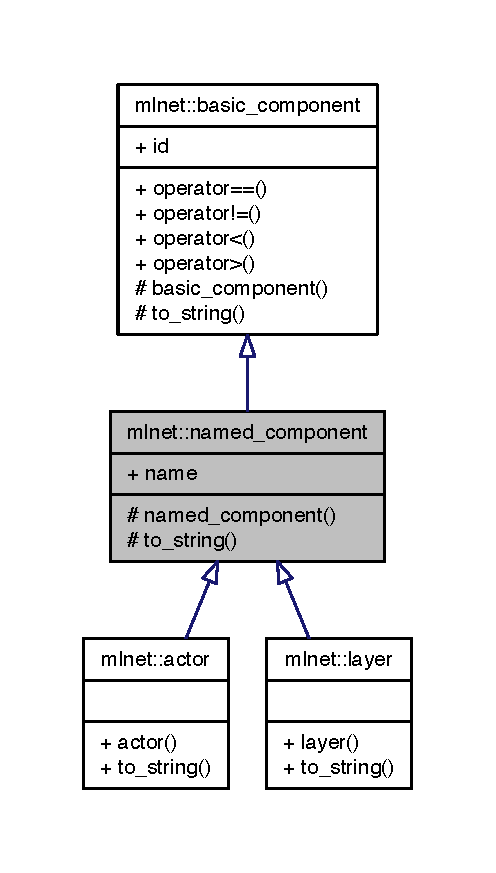
\includegraphics[width=238pt]{classmlnet_1_1named__component__inherit__graph}
\end{center}
\end{figure}


Collaboration diagram for mlnet\+:\+:named\+\_\+component\+:\nopagebreak
\begin{figure}[H]
\begin{center}
\leavevmode
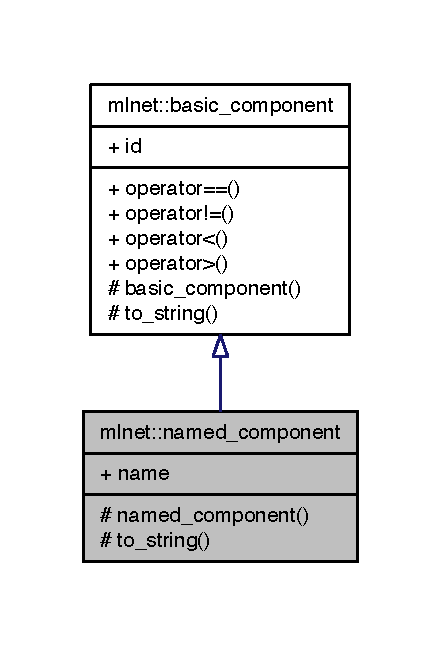
\includegraphics[width=212pt]{classmlnet_1_1named__component__coll__graph}
\end{center}
\end{figure}
\subsection*{Public Attributes}
\begin{DoxyCompactItemize}
\item 
const std\+::string \hyperlink{classmlnet_1_1named__component_a3015f6650729352abae8fb01e7ee7ca7}{name}
\end{DoxyCompactItemize}
\subsection*{Protected Member Functions}
\begin{DoxyCompactItemize}
\item 
\hyperlink{classmlnet_1_1named__component_a1333fc9ae4a272750e25f303ac619081}{named\+\_\+component} (const \hyperlink{namespacemlnet_a318fc9bfdb74e1da4d44d0c50d4a453d}{object\+\_\+id} \&\hyperlink{classmlnet_1_1basic__component_a7d56ea959ef686405bc0fa4830b03347}{id}, const std\+::string \&\hyperlink{classmlnet_1_1named__component_a3015f6650729352abae8fb01e7ee7ca7}{name})
\item 
std\+::string \hyperlink{classmlnet_1_1named__component_a46c630c6fe0ece5e8b3277ad3863112f}{to\+\_\+string} () const 
\end{DoxyCompactItemize}
\subsection*{Additional Inherited Members}


\subsection{Detailed Description}
A basic component of a \hyperlink{classmlnet_1_1_m_l_network}{M\+L\+Network}, which can be identified by name. 

\subsection{Constructor \& Destructor Documentation}
\hypertarget{classmlnet_1_1named__component_a1333fc9ae4a272750e25f303ac619081}{\index{mlnet\+::named\+\_\+component@{mlnet\+::named\+\_\+component}!named\+\_\+component@{named\+\_\+component}}
\index{named\+\_\+component@{named\+\_\+component}!mlnet\+::named\+\_\+component@{mlnet\+::named\+\_\+component}}
\subsubsection[{named\+\_\+component}]{\setlength{\rightskip}{0pt plus 5cm}mlnet\+::named\+\_\+component\+::named\+\_\+component (
\begin{DoxyParamCaption}
\item[{const {\bf object\+\_\+id} \&}]{id, }
\item[{const std\+::string \&}]{name}
\end{DoxyParamCaption}
)\hspace{0.3cm}{\ttfamily [protected]}}}\label{classmlnet_1_1named__component_a1333fc9ae4a272750e25f303ac619081}
Constructor 

\subsection{Member Function Documentation}
\hypertarget{classmlnet_1_1named__component_a46c630c6fe0ece5e8b3277ad3863112f}{\index{mlnet\+::named\+\_\+component@{mlnet\+::named\+\_\+component}!to\+\_\+string@{to\+\_\+string}}
\index{to\+\_\+string@{to\+\_\+string}!mlnet\+::named\+\_\+component@{mlnet\+::named\+\_\+component}}
\subsubsection[{to\+\_\+string}]{\setlength{\rightskip}{0pt plus 5cm}std\+::string mlnet\+::named\+\_\+component\+::to\+\_\+string (
\begin{DoxyParamCaption}
{}
\end{DoxyParamCaption}
) const\hspace{0.3cm}{\ttfamily [protected]}}}\label{classmlnet_1_1named__component_a46c630c6fe0ece5e8b3277ad3863112f}
Output function, presenting a complete description of the actor 

\subsection{Member Data Documentation}
\hypertarget{classmlnet_1_1named__component_a3015f6650729352abae8fb01e7ee7ca7}{\index{mlnet\+::named\+\_\+component@{mlnet\+::named\+\_\+component}!name@{name}}
\index{name@{name}!mlnet\+::named\+\_\+component@{mlnet\+::named\+\_\+component}}
\subsubsection[{name}]{\setlength{\rightskip}{0pt plus 5cm}const std\+::string mlnet\+::named\+\_\+component\+::name}}\label{classmlnet_1_1named__component_a3015f6650729352abae8fb01e7ee7ca7}
Unique name of the component 

The documentation for this class was generated from the following file\+:\begin{DoxyCompactItemize}
\item 
include/datastructures.\+h\end{DoxyCompactItemize}

\hypertarget{classmlnet_1_1node}{\section{mlnet\+:\+:node Class Reference}
\label{classmlnet_1_1node}\index{mlnet\+::node@{mlnet\+::node}}
}


{\ttfamily \#include $<$datastructures.\+h$>$}



Inheritance diagram for mlnet\+:\+:node\+:\nopagebreak
\begin{figure}[H]
\begin{center}
\leavevmode
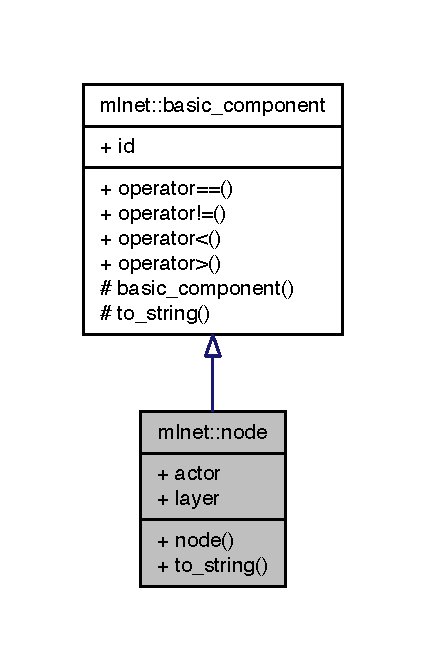
\includegraphics[width=204pt]{classmlnet_1_1node__inherit__graph}
\end{center}
\end{figure}


Collaboration diagram for mlnet\+:\+:node\+:\nopagebreak
\begin{figure}[H]
\begin{center}
\leavevmode
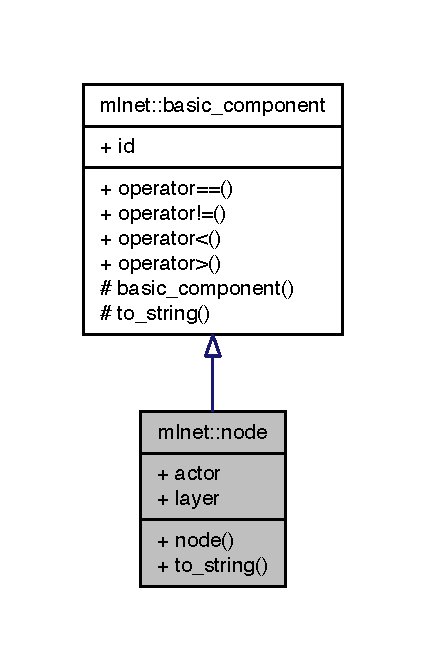
\includegraphics[width=204pt]{classmlnet_1_1node__coll__graph}
\end{center}
\end{figure}
\subsection*{Public Member Functions}
\begin{DoxyCompactItemize}
\item 
\hyperlink{classmlnet_1_1node_ac15d064db76b462b368ff88bf298a63f}{node} (const \hyperlink{namespacemlnet_a4c354f08ca868982bf3ddae882ff71c6}{node\+\_\+id} \&\hyperlink{classmlnet_1_1basic__component_a7d56ea959ef686405bc0fa4830b03347}{id}, const \hyperlink{namespacemlnet_a714fd98ffaeaadd5c38d61fa53dc4d24}{Actor\+Shared\+Ptr} \&\hyperlink{classmlnet_1_1actor}{actor}, const \hyperlink{namespacemlnet_a10c007fb811c55339dd5b9d32bb0505d}{Layer\+Shared\+Ptr} \&\hyperlink{classmlnet_1_1layer}{layer})
\item 
std\+::string \hyperlink{classmlnet_1_1node_ad5685fbd552276eb4adb1eae9b5851d3}{to\+\_\+string} () const 
\end{DoxyCompactItemize}
\subsection*{Public Attributes}
\begin{DoxyCompactItemize}
\item 
\hyperlink{namespacemlnet_a714fd98ffaeaadd5c38d61fa53dc4d24}{Actor\+Shared\+Ptr} \hyperlink{classmlnet_1_1node_a3d003cd3e2fc96297a4e3fe5a7c8d0b1}{actor}
\item 
\hyperlink{namespacemlnet_a10c007fb811c55339dd5b9d32bb0505d}{Layer\+Shared\+Ptr} \hyperlink{classmlnet_1_1node_ab7c3c0f9c8c0bd4952f764aa9215217e}{layer}
\end{DoxyCompactItemize}
\subsection*{Additional Inherited Members}


\subsection{Detailed Description}
A node inside a \hyperlink{classmlnet_1_1_m_l_network}{M\+L\+Network}. 

\subsection{Constructor \& Destructor Documentation}
\hypertarget{classmlnet_1_1node_ac15d064db76b462b368ff88bf298a63f}{\index{mlnet\+::node@{mlnet\+::node}!node@{node}}
\index{node@{node}!mlnet\+::node@{mlnet\+::node}}
\subsubsection[{node}]{\setlength{\rightskip}{0pt plus 5cm}mlnet\+::node\+::node (
\begin{DoxyParamCaption}
\item[{const {\bf node\+\_\+id} \&}]{id, }
\item[{const {\bf Actor\+Shared\+Ptr} \&}]{actor, }
\item[{const {\bf Layer\+Shared\+Ptr} \&}]{layer}
\end{DoxyParamCaption}
)}}\label{classmlnet_1_1node_ac15d064db76b462b368ff88bf298a63f}
Constructor 

\subsection{Member Function Documentation}
\hypertarget{classmlnet_1_1node_ad5685fbd552276eb4adb1eae9b5851d3}{\index{mlnet\+::node@{mlnet\+::node}!to\+\_\+string@{to\+\_\+string}}
\index{to\+\_\+string@{to\+\_\+string}!mlnet\+::node@{mlnet\+::node}}
\subsubsection[{to\+\_\+string}]{\setlength{\rightskip}{0pt plus 5cm}std\+::string mlnet\+::node\+::to\+\_\+string (
\begin{DoxyParamCaption}
{}
\end{DoxyParamCaption}
) const}}\label{classmlnet_1_1node_ad5685fbd552276eb4adb1eae9b5851d3}
Output function, presenting a complete description of the node 

\subsection{Member Data Documentation}
\hypertarget{classmlnet_1_1node_a3d003cd3e2fc96297a4e3fe5a7c8d0b1}{\index{mlnet\+::node@{mlnet\+::node}!actor@{actor}}
\index{actor@{actor}!mlnet\+::node@{mlnet\+::node}}
\subsubsection[{actor}]{\setlength{\rightskip}{0pt plus 5cm}{\bf Actor\+Shared\+Ptr} mlnet\+::node\+::actor}}\label{classmlnet_1_1node_a3d003cd3e2fc96297a4e3fe5a7c8d0b1}
The actor corresponding to this node \hypertarget{classmlnet_1_1node_ab7c3c0f9c8c0bd4952f764aa9215217e}{\index{mlnet\+::node@{mlnet\+::node}!layer@{layer}}
\index{layer@{layer}!mlnet\+::node@{mlnet\+::node}}
\subsubsection[{layer}]{\setlength{\rightskip}{0pt plus 5cm}{\bf Layer\+Shared\+Ptr} mlnet\+::node\+::layer}}\label{classmlnet_1_1node_ab7c3c0f9c8c0bd4952f764aa9215217e}
The layer where this node is located 

The documentation for this class was generated from the following file\+:\begin{DoxyCompactItemize}
\item 
include/datastructures.\+h\end{DoxyCompactItemize}

\hypertarget{class_operation_not_supported_exception}{\section{Operation\+Not\+Supported\+Exception Class Reference}
\label{class_operation_not_supported_exception}\index{Operation\+Not\+Supported\+Exception@{Operation\+Not\+Supported\+Exception}}
}


Inheritance diagram for Operation\+Not\+Supported\+Exception\+:\nopagebreak
\begin{figure}[H]
\begin{center}
\leavevmode
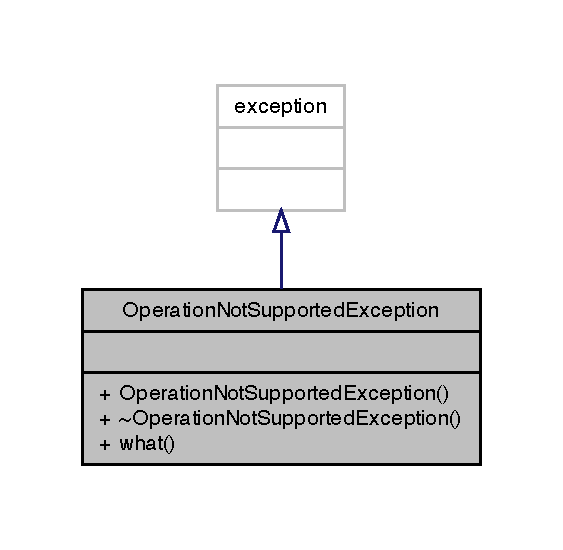
\includegraphics[width=270pt]{class_operation_not_supported_exception__inherit__graph}
\end{center}
\end{figure}


Collaboration diagram for Operation\+Not\+Supported\+Exception\+:\nopagebreak
\begin{figure}[H]
\begin{center}
\leavevmode
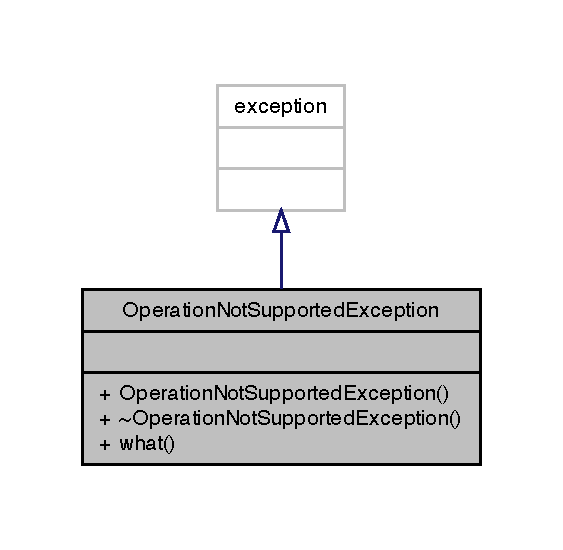
\includegraphics[width=270pt]{class_operation_not_supported_exception__coll__graph}
\end{center}
\end{figure}
\subsection*{Public Member Functions}
\begin{DoxyCompactItemize}
\item 
\hypertarget{class_operation_not_supported_exception_ab6f7474f05c4b91ac0f31c9e852bfedb}{{\bfseries Operation\+Not\+Supported\+Exception} (std\+::string value)}\label{class_operation_not_supported_exception_ab6f7474f05c4b91ac0f31c9e852bfedb}

\item 
\hypertarget{class_operation_not_supported_exception_ab6533734842e249902213a809a4d3f78}{virtual const char $\ast$ {\bfseries what} () const   throw ()}\label{class_operation_not_supported_exception_ab6533734842e249902213a809a4d3f78}

\end{DoxyCompactItemize}


The documentation for this class was generated from the following file\+:\begin{DoxyCompactItemize}
\item 
include/exceptions.\+h\end{DoxyCompactItemize}

\hypertarget{classmlnet_1_1_sorted_set}{\section{mlnet\+:\+:Sorted\+Set$<$ T $>$ Class Template Reference}
\label{classmlnet_1_1_sorted_set}\index{mlnet\+::\+Sorted\+Set$<$ T $>$@{mlnet\+::\+Sorted\+Set$<$ T $>$}}
}


{\ttfamily \#include $<$datastructures.\+h$>$}



Inheritance diagram for mlnet\+:\+:Sorted\+Set$<$ T $>$\+:\nopagebreak
\begin{figure}[H]
\begin{center}
\leavevmode
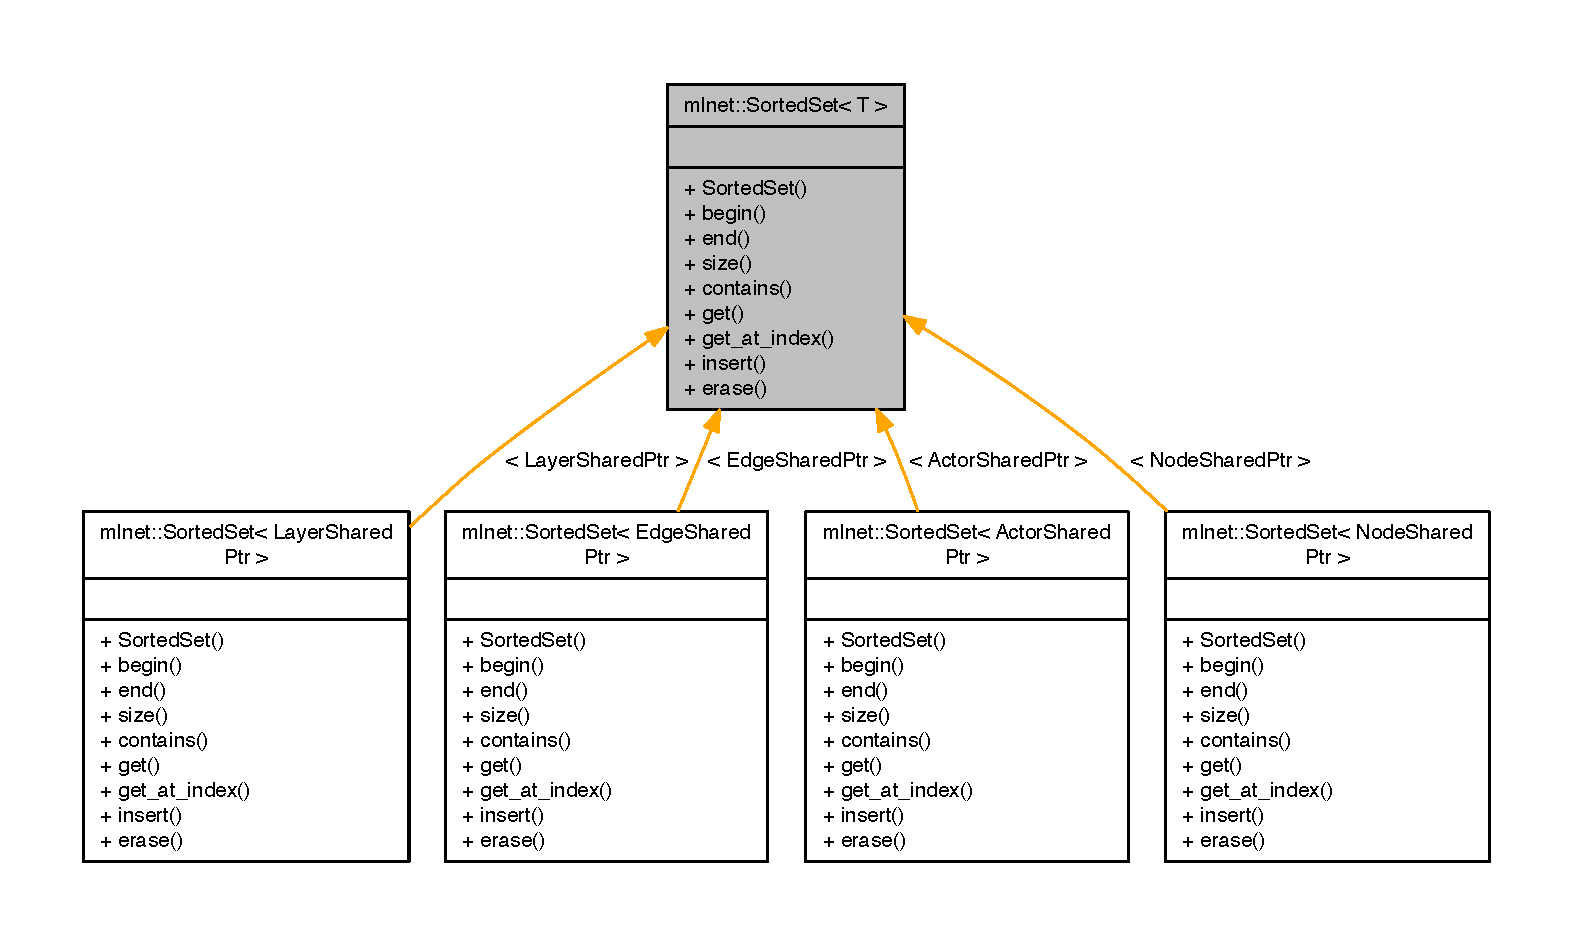
\includegraphics[width=350pt]{classmlnet_1_1_sorted_set__inherit__graph}
\end{center}
\end{figure}


Collaboration diagram for mlnet\+:\+:Sorted\+Set$<$ T $>$\+:\nopagebreak
\begin{figure}[H]
\begin{center}
\leavevmode
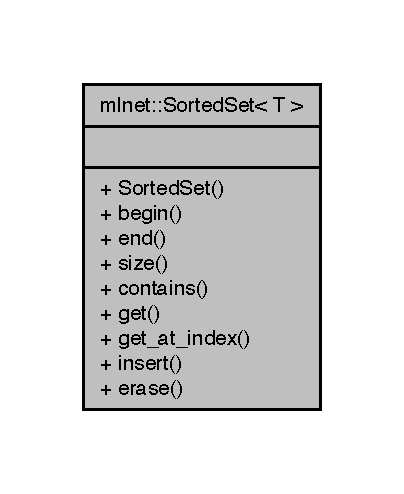
\includegraphics[width=194pt]{classmlnet_1_1_sorted_set__coll__graph}
\end{center}
\end{figure}
\subsection*{Classes}
\begin{DoxyCompactItemize}
\item 
class \hyperlink{classmlnet_1_1_sorted_set_1_1iterator}{iterator}
\end{DoxyCompactItemize}
\subsection*{Public Member Functions}
\begin{DoxyCompactItemize}
\item 
\hyperlink{classmlnet_1_1_sorted_set}{Sorted\+Set}$<$ T $>$\+::\hyperlink{classmlnet_1_1_sorted_set_1_1iterator}{iterator} \hyperlink{classmlnet_1_1_sorted_set_a15e228958332c123992f64df476324a3}{begin} () const 
\item 
\hyperlink{classmlnet_1_1_sorted_set}{Sorted\+Set}$<$ T $>$\+::\hyperlink{classmlnet_1_1_sorted_set_1_1iterator}{iterator} \hyperlink{classmlnet_1_1_sorted_set_ac88f8211ad1c259ee564320964085b58}{end} () const 
\item 
long \hyperlink{classmlnet_1_1_sorted_set_acd1e6023e51870488b53738d3609c784}{size} () const 
\item 
bool \hyperlink{classmlnet_1_1_sorted_set_a8d3dc2becc4da73e27ca44ef3dc0112c}{contains} (\hyperlink{namespacemlnet_a318fc9bfdb74e1da4d44d0c50d4a453d}{object\+\_\+id}) const 
\item 
T \hyperlink{classmlnet_1_1_sorted_set_a09a806a0625594688d7551a3cd2b6b6c}{get} (\hyperlink{namespacemlnet_a318fc9bfdb74e1da4d44d0c50d4a453d}{object\+\_\+id}) const 
\item 
T \hyperlink{classmlnet_1_1_sorted_set_a2268be8183ea413d6c85a41051f8bc2e}{get\+\_\+at\+\_\+index} (long) const 
\item 
void \hyperlink{classmlnet_1_1_sorted_set_a463ccc94cdfb56b0c45c418f91067fc8}{insert} (\hyperlink{namespacemlnet_a318fc9bfdb74e1da4d44d0c50d4a453d}{object\+\_\+id}, T)
\item 
void \hyperlink{classmlnet_1_1_sorted_set_a0ff289209df1bc8f890078a31eca3e44}{erase} (\hyperlink{namespacemlnet_a318fc9bfdb74e1da4d44d0c50d4a453d}{object\+\_\+id})
\end{DoxyCompactItemize}


\subsection{Detailed Description}
\subsubsection*{template$<$class T$>$class mlnet\+::\+Sorted\+Set$<$ T $>$}

Sorted Set A \hyperlink{classmlnet_1_1_sorted_set}{Sorted\+Set} is a class used to store a set of components that\+:
\begin{DoxyEnumerate}
\item can be accessed by id in log time.
\item can be accessed by index (position) in the set in constant time.
\item can be accessed using a const iterator, so that it is not necessary to duplicate them. As an example, it is not necessary to duplicate nodes when the neighbors of a node are accessed\+: a \hyperlink{classmlnet_1_1_sorted_set}{Sorted\+Set} on those nodes is returned instead.
\end{DoxyEnumerate}

A \hyperlink{classmlnet_1_1_sorted_set}{Sorted\+Set} is implemented as a skip list.

A \hyperlink{classmlnet_1_1_sorted_set}{Sorted\+Set} is a class used to store a set of components that\+:
\begin{DoxyEnumerate}
\item can be accessed by id in log time.
\item can be accessed by index (position) in the set in constant time.
\item can be accessed using a const iterator, so that it is not necessary to duplicate them. As an example, it is not necessary to duplicate nodes when the neighbors of a node are accessed\+: a \hyperlink{classmlnet_1_1_sorted_set}{Sorted\+Set} on those nodes is returned instead.
\end{DoxyEnumerate}

A \hyperlink{classmlnet_1_1_sorted_set}{Sorted\+Set} is implemented as a skip list. 

\subsection{Member Function Documentation}
\hypertarget{classmlnet_1_1_sorted_set_a15e228958332c123992f64df476324a3}{\index{mlnet\+::\+Sorted\+Set@{mlnet\+::\+Sorted\+Set}!begin@{begin}}
\index{begin@{begin}!mlnet\+::\+Sorted\+Set@{mlnet\+::\+Sorted\+Set}}
\subsubsection[{begin}]{\setlength{\rightskip}{0pt plus 5cm}template$<$class T $>$ {\bf Sorted\+Set}$<$ T $>$\+::{\bf iterator} Sorted\+Set\+::begin (
\begin{DoxyParamCaption}
{}
\end{DoxyParamCaption}
) const}}\label{classmlnet_1_1_sorted_set_a15e228958332c123992f64df476324a3}
Returns an iterator to the first object in the collection \hypertarget{classmlnet_1_1_sorted_set_a8d3dc2becc4da73e27ca44ef3dc0112c}{\index{mlnet\+::\+Sorted\+Set@{mlnet\+::\+Sorted\+Set}!contains@{contains}}
\index{contains@{contains}!mlnet\+::\+Sorted\+Set@{mlnet\+::\+Sorted\+Set}}
\subsubsection[{contains}]{\setlength{\rightskip}{0pt plus 5cm}template$<$class T $>$ bool Sorted\+Set\+::contains (
\begin{DoxyParamCaption}
\item[{{\bf object\+\_\+id}}]{search\+\_\+value}
\end{DoxyParamCaption}
) const}}\label{classmlnet_1_1_sorted_set_a8d3dc2becc4da73e27ca44ef3dc0112c}
Returns true if an obect with the input id is present in the collection \hypertarget{classmlnet_1_1_sorted_set_ac88f8211ad1c259ee564320964085b58}{\index{mlnet\+::\+Sorted\+Set@{mlnet\+::\+Sorted\+Set}!end@{end}}
\index{end@{end}!mlnet\+::\+Sorted\+Set@{mlnet\+::\+Sorted\+Set}}
\subsubsection[{end}]{\setlength{\rightskip}{0pt plus 5cm}template$<$class T $>$ {\bf Sorted\+Set}$<$ T $>$\+::{\bf iterator} Sorted\+Set\+::end (
\begin{DoxyParamCaption}
{}
\end{DoxyParamCaption}
) const}}\label{classmlnet_1_1_sorted_set_ac88f8211ad1c259ee564320964085b58}
Returns an iterator after the last object in the collection \hypertarget{classmlnet_1_1_sorted_set_a0ff289209df1bc8f890078a31eca3e44}{\index{mlnet\+::\+Sorted\+Set@{mlnet\+::\+Sorted\+Set}!erase@{erase}}
\index{erase@{erase}!mlnet\+::\+Sorted\+Set@{mlnet\+::\+Sorted\+Set}}
\subsubsection[{erase}]{\setlength{\rightskip}{0pt plus 5cm}template$<$class T $>$ void Sorted\+Set\+::erase (
\begin{DoxyParamCaption}
\item[{{\bf object\+\_\+id}}]{value}
\end{DoxyParamCaption}
)}}\label{classmlnet_1_1_sorted_set_a0ff289209df1bc8f890078a31eca3e44}
Removes the input object from the collection \hypertarget{classmlnet_1_1_sorted_set_a09a806a0625594688d7551a3cd2b6b6c}{\index{mlnet\+::\+Sorted\+Set@{mlnet\+::\+Sorted\+Set}!get@{get}}
\index{get@{get}!mlnet\+::\+Sorted\+Set@{mlnet\+::\+Sorted\+Set}}
\subsubsection[{get}]{\setlength{\rightskip}{0pt plus 5cm}template$<$class T $>$ T Sorted\+Set\+::get (
\begin{DoxyParamCaption}
\item[{{\bf object\+\_\+id}}]{search\+\_\+value}
\end{DoxyParamCaption}
) const}}\label{classmlnet_1_1_sorted_set_a09a806a0625594688d7551a3cd2b6b6c}
Returns the obect with the input id if it is present in the collection, or N\+U\+L\+L \hypertarget{classmlnet_1_1_sorted_set_a2268be8183ea413d6c85a41051f8bc2e}{\index{mlnet\+::\+Sorted\+Set@{mlnet\+::\+Sorted\+Set}!get\+\_\+at\+\_\+index@{get\+\_\+at\+\_\+index}}
\index{get\+\_\+at\+\_\+index@{get\+\_\+at\+\_\+index}!mlnet\+::\+Sorted\+Set@{mlnet\+::\+Sorted\+Set}}
\subsubsection[{get\+\_\+at\+\_\+index}]{\setlength{\rightskip}{0pt plus 5cm}template$<$class T $>$ T Sorted\+Set\+::get\+\_\+at\+\_\+index (
\begin{DoxyParamCaption}
\item[{long}]{pos}
\end{DoxyParamCaption}
) const}}\label{classmlnet_1_1_sorted_set_a2268be8183ea413d6c85a41051f8bc2e}
Returns the obect at the given position in the collection, or N\+U\+L\+L \hypertarget{classmlnet_1_1_sorted_set_a463ccc94cdfb56b0c45c418f91067fc8}{\index{mlnet\+::\+Sorted\+Set@{mlnet\+::\+Sorted\+Set}!insert@{insert}}
\index{insert@{insert}!mlnet\+::\+Sorted\+Set@{mlnet\+::\+Sorted\+Set}}
\subsubsection[{insert}]{\setlength{\rightskip}{0pt plus 5cm}template$<$class T$>$ void Sorted\+Set\+::insert (
\begin{DoxyParamCaption}
\item[{{\bf object\+\_\+id}}]{value, }
\item[{T}]{obj\+\_\+ptr}
\end{DoxyParamCaption}
)}}\label{classmlnet_1_1_sorted_set_a463ccc94cdfb56b0c45c418f91067fc8}
Inserts a new object in the collection \hypertarget{classmlnet_1_1_sorted_set_acd1e6023e51870488b53738d3609c784}{\index{mlnet\+::\+Sorted\+Set@{mlnet\+::\+Sorted\+Set}!size@{size}}
\index{size@{size}!mlnet\+::\+Sorted\+Set@{mlnet\+::\+Sorted\+Set}}
\subsubsection[{size}]{\setlength{\rightskip}{0pt plus 5cm}template$<$class T $>$ long Sorted\+Set\+::size (
\begin{DoxyParamCaption}
{}
\end{DoxyParamCaption}
) const}}\label{classmlnet_1_1_sorted_set_acd1e6023e51870488b53738d3609c784}
Returns the number of objects in the collection 

The documentation for this class was generated from the following files\+:\begin{DoxyCompactItemize}
\item 
include/datastructures.\+h\item 
include/sortedset.\+cpp\end{DoxyCompactItemize}

\hypertarget{classmlnet_1_1_uniform_evolution_model}{\section{mlnet\+:\+:Uniform\+Evolution\+Model Class Reference}
\label{classmlnet_1_1_uniform_evolution_model}\index{mlnet\+::\+Uniform\+Evolution\+Model@{mlnet\+::\+Uniform\+Evolution\+Model}}
}


Grows a network by first creating all the vertexes and then at every step choosing two (uniform probability) to connect with an edge.  




{\ttfamily \#include $<$evolution.\+h$>$}



Inheritance diagram for mlnet\+:\+:Uniform\+Evolution\+Model\+:\nopagebreak
\begin{figure}[H]
\begin{center}
\leavevmode
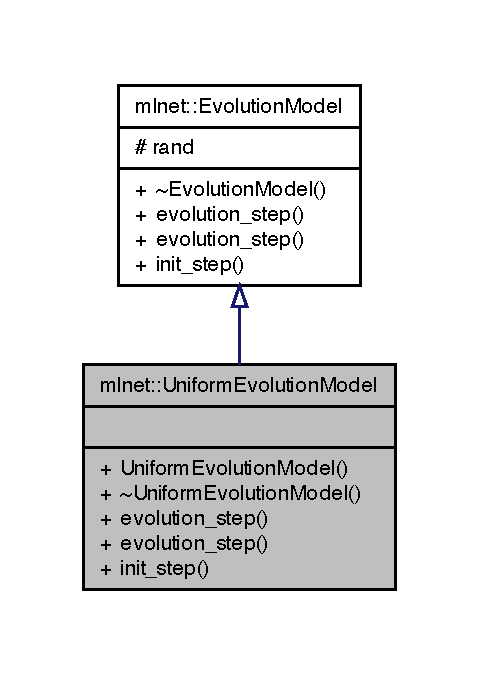
\includegraphics[width=230pt]{classmlnet_1_1_uniform_evolution_model__inherit__graph}
\end{center}
\end{figure}


Collaboration diagram for mlnet\+:\+:Uniform\+Evolution\+Model\+:\nopagebreak
\begin{figure}[H]
\begin{center}
\leavevmode
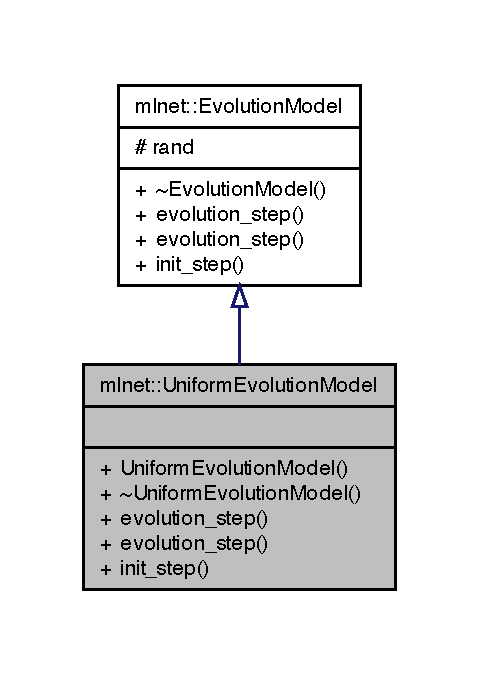
\includegraphics[width=230pt]{classmlnet_1_1_uniform_evolution_model__coll__graph}
\end{center}
\end{figure}
\subsection*{Public Member Functions}
\begin{DoxyCompactItemize}
\item 
\hypertarget{classmlnet_1_1_uniform_evolution_model_a9686b3e7b297645a5864c6bf5bd167a3}{{\bfseries Uniform\+Evolution\+Model} (int m0)}\label{classmlnet_1_1_uniform_evolution_model_a9686b3e7b297645a5864c6bf5bd167a3}

\item 
\hypertarget{classmlnet_1_1_uniform_evolution_model_ae71cabef018c2465c0d1a54ff181002d}{void {\bfseries evolution\+\_\+step} (\hyperlink{classmlnet_1_1_m_l_network}{M\+L\+Network} \&mnet, \hyperlink{namespacemlnet_a84ad9c6056f0eb7d129995351f9b13fb}{layer\+\_\+id} net)}\label{classmlnet_1_1_uniform_evolution_model_ae71cabef018c2465c0d1a54ff181002d}

\item 
\hypertarget{classmlnet_1_1_uniform_evolution_model_ae29f442e24771508fe516eae962ae053}{void {\bfseries evolution\+\_\+step} (\hyperlink{classmlnet_1_1_m_l_network}{M\+L\+Network} \&mnet, \hyperlink{namespacemlnet_a84ad9c6056f0eb7d129995351f9b13fb}{layer\+\_\+id} net, std\+::set$<$ \hyperlink{namespacemlnet_a4c354f08ca868982bf3ddae882ff71c6}{node\+\_\+id} $>$ \&new\+\_\+vertexes, std\+::set$<$ \hyperlink{namespacemlnet_ad708e58e72680351e102e6b3d0489145}{edge\+\_\+id} $>$ \&new\+\_\+edges)}\label{classmlnet_1_1_uniform_evolution_model_ae29f442e24771508fe516eae962ae053}

\item 
\hypertarget{classmlnet_1_1_uniform_evolution_model_a9563111b1399676538324f847a114054}{void {\bfseries init\+\_\+step} (\hyperlink{classmlnet_1_1_m_l_network}{M\+L\+Network} \&mnet, \hyperlink{namespacemlnet_a84ad9c6056f0eb7d129995351f9b13fb}{layer\+\_\+id} net)}\label{classmlnet_1_1_uniform_evolution_model_a9563111b1399676538324f847a114054}

\end{DoxyCompactItemize}
\subsection*{Additional Inherited Members}


\subsection{Detailed Description}
Grows a network by first creating all the vertexes and then at every step choosing two (uniform probability) to connect with an edge. 

The documentation for this class was generated from the following file\+:\begin{DoxyCompactItemize}
\item 
include/evolution.\+h\end{DoxyCompactItemize}

\hypertarget{class_wrong_format_exception}{\section{Wrong\+Format\+Exception Class Reference}
\label{class_wrong_format_exception}\index{Wrong\+Format\+Exception@{Wrong\+Format\+Exception}}
}


Inheritance diagram for Wrong\+Format\+Exception\+:\nopagebreak
\begin{figure}[H]
\begin{center}
\leavevmode
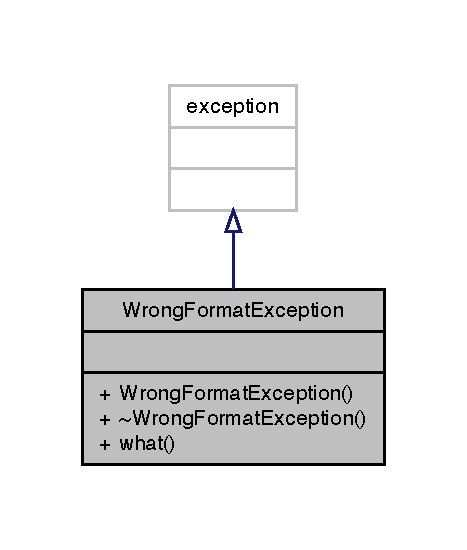
\includegraphics[width=224pt]{class_wrong_format_exception__inherit__graph}
\end{center}
\end{figure}


Collaboration diagram for Wrong\+Format\+Exception\+:\nopagebreak
\begin{figure}[H]
\begin{center}
\leavevmode
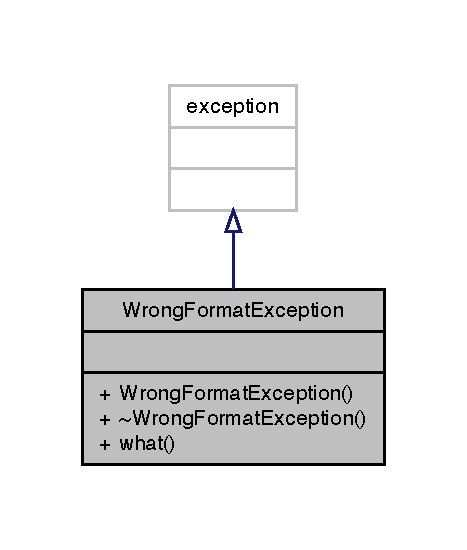
\includegraphics[width=224pt]{class_wrong_format_exception__coll__graph}
\end{center}
\end{figure}
\subsection*{Public Member Functions}
\begin{DoxyCompactItemize}
\item 
\hypertarget{class_wrong_format_exception_ac4629be19e1e2238a78a26a36b460d44}{{\bfseries Wrong\+Format\+Exception} (std\+::string path)}\label{class_wrong_format_exception_ac4629be19e1e2238a78a26a36b460d44}

\item 
\hypertarget{class_wrong_format_exception_a26013218831b9785f02bd5c26e938492}{virtual const char $\ast$ {\bfseries what} () const   throw ()}\label{class_wrong_format_exception_a26013218831b9785f02bd5c26e938492}

\end{DoxyCompactItemize}


The documentation for this class was generated from the following file\+:\begin{DoxyCompactItemize}
\item 
include/exceptions.\+h\end{DoxyCompactItemize}

\hypertarget{class_wrong_parameter_exception}{\section{Wrong\+Parameter\+Exception Class Reference}
\label{class_wrong_parameter_exception}\index{Wrong\+Parameter\+Exception@{Wrong\+Parameter\+Exception}}
}


Inheritance diagram for Wrong\+Parameter\+Exception\+:\nopagebreak
\begin{figure}[H]
\begin{center}
\leavevmode
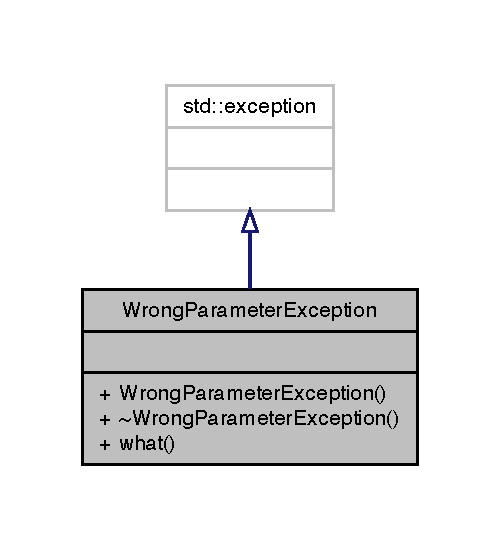
\includegraphics[width=240pt]{class_wrong_parameter_exception__inherit__graph}
\end{center}
\end{figure}


Collaboration diagram for Wrong\+Parameter\+Exception\+:\nopagebreak
\begin{figure}[H]
\begin{center}
\leavevmode
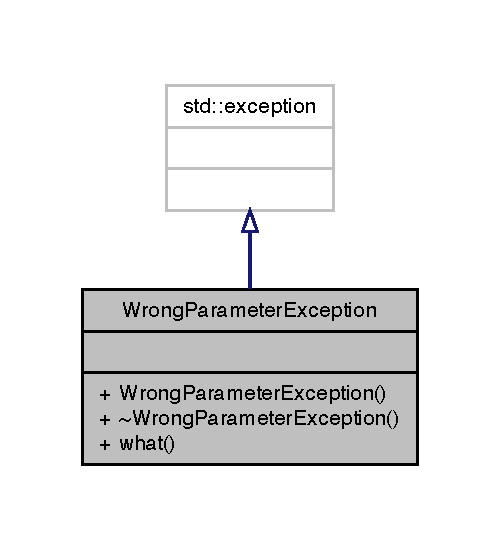
\includegraphics[width=240pt]{class_wrong_parameter_exception__coll__graph}
\end{center}
\end{figure}
\subsection*{Public Member Functions}
\begin{DoxyCompactItemize}
\item 
\hypertarget{class_wrong_parameter_exception_a228fb340058bbb9b53adeabc56616099}{{\bfseries Wrong\+Parameter\+Exception} (std\+::string value)}\label{class_wrong_parameter_exception_a228fb340058bbb9b53adeabc56616099}

\item 
\hypertarget{class_wrong_parameter_exception_a7f79b5c6b6a8ac90bb51e00948d4dc29}{virtual const char $\ast$ {\bfseries what} () const   throw ()}\label{class_wrong_parameter_exception_a7f79b5c6b6a8ac90bb51e00948d4dc29}

\end{DoxyCompactItemize}


The documentation for this class was generated from the following file\+:\begin{DoxyCompactItemize}
\item 
include/exceptions.\+h\end{DoxyCompactItemize}

%--- End generated contents ---

% Index
\newpage
\phantomsection
\addcontentsline{toc}{chapter}{Index}
\printindex

\end{document}
